\documentclass[12pt,twoside]{article}
\usepackage{jmlda}
\usepackage{tabularx}
\usepackage{ dsfont }
%\NOREVIEWERNOTES
\title
    {Раннее прогнозирование достаточного объема выборки для обобщенной линейной модели.}
\author
    {Бучнев~В.\,С., Грабовой~А.\,В., Гадаев~Т.\,Т., Стрижов~В.\,В.} % основной список авторов, выводимый в оглавление


\abstract
    {Исследуется проблема снижения затрат на сбор данных, необходимых для построения
адекватной модели. Рассматриваются задачи линейной и логистической моделей. Для решения этих задач требуется, чтобы выборка содержала необходимое число  объектов. Требуется предложить метод вычисления оптимального обьема данных, соблюдая при этом баланс между точностью модели и и трудозатратами при сборе данных. Предпочтительны те методы оценки объемы, которые позволяют строить адекватные модели по выборкам возможно меньшего объема.

\bigskip
\textbf{Ключевые слова}: \emph {Обобщенная линейная модель, размер выборки, байесовские методы, бутстреп}.}
\titleEng
    {JMLDA paper example: file jmlda-example.tex}
\authorEng
    {Author~F.\,S.$^1$, CoAuthor~F.\,S.$^2$, Name~F.\,S.$^2$}
\organizationEng
    {$^1$Organization; $^2$Organization}
\abstractEng
    {This document is an example of paper prepared with \LaTeXe\
    typesetting system and style file \texttt{jmlda.sty}.

    \bigskip
    \textbf{Keywords}: \emph{keyword, keyword, more keywords}.}
\begin{document}
\maketitle
%\linenumbers

\section{Введение}
При планировании эксперимента требуется оценить минимальный объём выборки — число производимых измерений набора показателей или признаков, необходимый для построениие сформулированных условий. 

Существует большое количество оценки размера выборки. Например, тест множителей Лагранжа, тест отношения правдоподобия и тест Вальда. В работах \cite{Self-Mauritsen-1998, Shieh-2000, Shieh-2005} на основе данных методов построена оценка оптимального размера выборки. Основной минус этих методов заключается в том, что статистики, используемые в критериях, имеют асимптотическое распределение и требуют большого обьема выборки.

Существуют также байесовские оценки обьема выборки: критерий средней апостериорной дисперсии, критерий среднего покрытия, критерий средней длины и метод максимизации полезности. Первые три метода требуют анализа некоторой функции эффективности от размера выборки. Используя некоторое решающее правило, по данной функции определяется достаточный объем выборки. Главный минус этих методов заключается в том, что они не позволяют построить аппроксимацию функции эффективности при большем объеме данных. Метод максимизации полезности максимизирует ожидание некоторой функции полезности по обьему выборки. Все эти методы опираются на апостериорное распределение, что требует достаточно большого обьема выборки.

Предлагается исследовать зависимость среднего значения логарифма правдоподобия от размера доступной выборки, а также его дисперсию. В данной работе предлагается использовать не сами функции эффективности, а их аппроксимации. Для этого предлагается использовать аппроксимацию ковариационной матрицы вектора параметров. После чего аппроксимировать данные две зависимости при помощи метода бутстреп. Для вычислительного эксперимента предлагается использовать классические выборки из UCI репозитория и синтетические данные.

\section{Постановка задачи}

Дана выборка размера $m$:

$$
\mathfrak D = \{\mathbf{x}_i, y_i\}_{i=1}^m,
$$

где $\textbf{x}_i \in \mathbb{R}^{n}$ --- вектор признаков, $~y_i \in \mathbb{Y}$.


Выборка является простой: элементы порождены независимо из одного распределения с фиксированными неизвестными параметрами, вероятность попадания каждого элемента в выборку одинакова. Предполагается, что выборка $\mathfrak D$ порождена согласно следующей гипотезе: модель, порождающая данные, задается в следующем виде:

\begin{equation}\label{f}
y_i = f(\mathbf{x}_i, \mathbf{w}, \beta),
\end{equation}
где $\textbf{w} \in \mathbb{W}$ --- вектор параметров, $\beta$ --- дисперсия зависимой переменной. Зависимая переменная $y$ аппроксимируется обобщенно линейной моделью:

\begin{equation}\label{y_f}
\hat{y_i} = f(\mathbf{x}_i, \mathbf{w}) = \mu(\mathbf{w}^{\top}\mathbf{x}_i),
\end{equation}
где $\mu$ --- функция связи, для модели линейной регрессии:

\begin{equation}\label{lin_reg_lf}
 \mu = id,
\end{equation}
для логистической регрессии:
\begin{equation}\label{log_reg_lf}
\mu(\mathbf{w}^{\top}\mathbf{x}_i) = \frac{1}{1 + \exp(-\mathbf{w}^{\top}\mathbf{x}_i)}.
\end{equation}

%Рассмотрим параметрическое семейство функций для модели линейной регрессии:
Предпологается, что при восстановлении параметров линейной регрессии (\ref{lin_reg_lf}), зависимая переменная порождается нормальным распределением:
$$
p(y | \mathbf{x}, \mathbf{w}) \sim \mathcal{N}(f(\mathbf{x}, \mathbf{w}), \hat{\beta}),
$$
где $\hat{\beta}$ --- выборочная дисперсия зависимой переменной $y$. Для модели логистической регрессии зависимая переменная порождается бернуллиевским распределением:
$$
p(y | \mathbf{x}, \mathbf{w}) \sim \mathcal{B}e \bigl( f(\mathbf{x}, \mathbf{w})\bigr).
$$

%$$
%\mathfrak{F} = \left\{f(y, \textbf{x}, \textbf{w}) | \textbf{w} \in \mathbb{W}, \int_{y \in \mathbb{Y}, \textbf{x} \in \mathbb{R}^n} f(y, \textbf{x}, \textbf{w})dyd\textbf{x} = 1\right\}.
%$$

Для модели $f$ с вектором параметров $\textbf{w}$ определим функцию правдоподобия и логарифмическую функцию правдоподобия выборки $\mathfrak D$:
\begin{equation}\label{L_l}
L(\textbf{w} | \mathfrak D) = \prod_{y, \textbf{x} \in \mathfrak D} p(y | \textbf{x}, \textbf{w}),~~~ l(\textbf w | \mathfrak D) = \sum_{y, \textbf{x} \in \mathfrak D}\log p(y | \textbf{x}, \textbf{w}).
\end{equation}

%Рассмотрим правдоподобие выборки $\mathfrak D_{\mathcal L_m}$:

%$$
%L(\mathfrak D_{\mathcal T_m}, \mathfrak D_{\mathcal L_m}) = \prod_{y, \textbf{x} \in \mathfrak D_{\mathcal T_m}} f(y, \textbf{x},  \textbf{w}).
%$$

%Рассмотрим логарифм правдоподобия выборки $\mathfrak D_{\mathcal L_m}$:

%$$
%l(\mathfrak D_{\mathcal T_m}, \textbf w) = \sum_{y, \textbf{x} \in \mathfrak D_{\mathcal T_m}}\log f(y, \textbf{x}, \textbf{w}).
%$$

%Будем рассматривать ожидаемое значение функции $l$:

%$$
%\tilde{l}(\mathfrak D)  = \underset{y, \textbf{x} \in \mathfrak D}{\mathsf E} l(\{y, \textbf{x}\}, \textbf w).
%$$

Для множества индексов $\mathcal{A}$ независимой переменной $\mathbf{x} = [x_1, ..., x_n]^{\top}$, в векторы $\mathbf{x}_{\mathcal{A}}, \mathbf{w}_{\mathcal{A}}$ входят только те элементы, индексы которых принадлежат $\mathcal{A}$. Определим выборку $\mathfrak{D}_{\mathcal{A}}$ как множество независимых переменных $\mathbf{x}_{\mathcal{A}}$ и соответствующих им зависимых переменных $y$.

%$$
%\mathbf{w}_{\mathcal{A}} = (\mathbf{w}_{a_1}, ..., \mathbf{w}_{a_k}),
%$$
%$$
%\mathbf{x}_{i{\mathcal{A}}} = (\mathbf{x}_{i{a_1}}, ..., \mathbf{x}_{i{a_k}}),
%$$
%$$
%\mathbf{x}_{\mathcal{A}} = (\mathbf{x}_{1\mathcal{A}}, ..., \mathbf{x}_{m\mathcal{A}})^{\top},
%$$
%$$
%\mathfrak{D}_{\mathcal{A}} =  \{\mathbf{x}_{i\mathcal{A}}, y_i\}_{i=1}^m,
%$$

Для получения оптимального набора параметров и оценки вектора параметров используется принцип максимума правдоподобия:

\begin{equation}\label{argmax_L}
\hat{\textbf{w}}, \hat{\mathcal{A}} = \argmax_{\mathbf{w} \in \mathbb{W}, \mathcal{A} \subseteq \mathbb{J}} L(\textbf{w}_{\mathcal{A}} | \mathfrak D_{\mathcal{A}}),
\end{equation}
где $\mathbb{J} = \{1, 2, ..., n\}$ --- множество индексов.

%Оптимизационная задача (\ref{argmax_L}) эквивалентна оптимизационной задаче:
%\begin{equation}\label{argmin_MSE}
%\hat{\mathbf{w}}, \hat{\mathcal{A}} = \argmin_{\mathbf{w} \in \mathbb{W}, \mathcal{A} \subseteq \mathbb{J}} MSE(\mathbf{x}%_{\mathcal{A}}, y, \mathbf{w}_{\mathcal{A}}),
%\end{equation}
%где $MSE(\mathbf{x}, y, \mathbf{w})$ --- функция ошибки:
В качестве функции ошибки используются следующие функции:
\begin{equation}\label{MSE_CE}
S_{\text{reg}}(\mathbf{x}, y, \textbf{w}) = \frac{1}{m}\sum\limits_{i=1}^{m}(y_i - \textbf{w}^{\top}\mathbf{x}_i )^2, ~~~ S_{\text{class}} = \sum\limits_{i=1}^{m}(y_i\ln f(\mathbf{x}_i, \mathbf{w}) + (1 - y_i)\ln(1 - f(\mathbf{x}_i, \mathbf{w}))).
\end{equation}

Требуется по начально заданной выборке размера $m_0 \ll m$ получить оценку минимального достаточного объёма $m^{*}$. Для введения понятия достаточности объёма  выборки рассмотрим ожидаемое значение усредненного логарифма правдоподобия (\ref{L_l}) по разным подвыборкам $\mathfrak D^{\prime}$ размера $m_0$ обучающей выборки $\mathfrak{D}$ на оценке вектора параметров $\hat{\mathbf{w}}$:

$$
l(m_0) = m_0^{-1}\underset{|\mathfrak D^{\prime}| = m_0}{\underset{\mathfrak D^{\prime} \subset \mathfrak D}{\mathsf E}} l(\hat{\mathbf{w}} | \mathfrak D^{\prime}).
$$

Будем считать, что объем выборки достаточен, если:

$$
\forall m_1, m_2 > m^* ~~~ |l(m_1) - l(m_2)| < \delta,
$$
где $\delta$ --- достаточно малое пороговое значение.

Для получения аппроксимации функции $l(m_0)$ по выборке $\mathfrak D_{m_0}$ введем процедуру бутстрепа:

\begin{enumerate}
	\item Из равномерного распределения генерируется случайный вектор индексов 
$$
\mathbf{i} = (i_1, ..., i_{m_0}),
$$
где:
	\begin{itemize}
		\item $i_j \sim U(\{1, ..., m\})$ --- вариант 1,
		\item $i_j \sim U(\{1, ..., m_0\})$ --- вариант 2.
	\end{itemize}
	\item Для полученной выборки $\mathfrak D_{\mathbf{i}} = \{\mathbf{x}_{i_j}, y_{i_j}\}_{j=1}^{m_0}$ считается усредненный логарифм правдоподобия на оценке вектора параметров $\hat{\mathbf{w}}$:
$$
\hat{l}_{k}(m_0) = \frac{1}{m_0}l(\hat{\mathbf{w}} | \mathfrak D_{\mathbf{i}})
$$
	\item пп. 1-2 повторяются $K$ раз, оценка $\hat{l}(m_0)$ функции $l(m_0)$ задается формулой:
$$
\hat{l}(m_0) = \frac{1}{K}\sum\limits_{k=1}^K \hat{l}_{k}(m_0).
$$
\end{enumerate}

Для предсказания значения функции $\hat{l}(m)$ при $m > m_0$ введем семейство функций $\Phi = \{\phi(m) =  a + b\cdot m^c ~|~ a, b \in \mathbb{R}, c \in (-\infty, 0)\}$
Функция $\hat{l}$ приближается функцией вида:

\begin{equation}\label{argmin_MAPE}
\hat{\phi} =  \argmin_{\phi \in \Phi}\text{MAPE}(\hat{l}, \phi, 1, m_0),
\end{equation}
где $\text{MAPE}$ --- средняя абсолютная процентная ошибка:
\begin{equation}\label{MAPE}
\text{MAPE}(\psi, \phi, m_1, m_2) = \frac{1}{m_2 - m_1 + 1}\sum_{i=m_1}^{m_2}\frac{|\phi(i) - \psi(i)|}{\psi(i)}.
\end{equation}

%Рассмотрим матрицу информации Фишера:

%$$
%\textbf{I}(\mathfrak D, \textbf{w}) = -\nabla\nabla l(\mathfrak D, \textbf{w}).
%$$

%Будем считать, что $\hat{\textbf{w}}$ имеет следующее распределение:

%$$
%\hat{\textbf{w}} \sim \mathcal{N}(\textbf{m}, \textbf{V}),~~~ \textbf{V} = \textbf{I}^{-1}(\mathfrak D, m).
%$$

%Для линейной регрессии $\mathbb{Y} = \mathbb{R}$, где $y$ представимо в виде:

%$$
%y = \textbf{x}^{\top}\textbf{w} + \epsilon,
%$$
%где $\epsilon \sim \mathcal{N}(0, 1)$. 

%Аппроксимация плотности апостериорной вероятности имеет вид:

%$$
%f(y, \textbf{x}, \textbf{w}) = \mathcal{N}(y|\textbf{x}^{\top}\textbf{w}, 1).
%$$ 

%Для логистической регрессии $\mathbb{Y} = \{0, 1\}$, где $y$ является бернуллиевской случайной величиной:

%$$
%y \sim \mathcal{B}e(\theta),
%$$
%где $\theta$ - неизвестный параметр распределения. Аппроксимация плотности апостериорной вероятности имеет вид:

%$$
%f(y, \textbf{x}, \textbf{w}) = \mathcal{B}e(y|\theta),~~~ \theta = \frac{1}{1 + exp(-\textbf{x}^{\top}\textbf{w})}.
%$$

\section{Анализ эффективности модели}

Методы байесовских оценок объема выборки основаны на ограничении некоторой выбранной характеристики модели. Для анализа эффективности вводится функция от объема выборки, увеличение значений которой интерпретируется как уменьшение эффективности модели. Объем выборки $m^{*}$ выбирается таким, при котором исследуемая функция не превышает некоторого порогового значения $\epsilon$.

\subsection{Критерий средней длины (ALC)}

Пусть $A(\mathfrak{D}) \subset \mathbb{R}^n$ --- множество значений параметров модели \textbf{w}:

$$
A(\mathfrak{D}) = \{\textbf{w} : ||\textbf{w}- \hat{\textbf{w}}|| \leqslant r_m\}
$$
такое, что
$$
\mathsf{P}(A(\mathfrak{D})) = 1 - \alpha,
$$
где $\alpha$ --- некоторое малое значение. 

Критерий средней длины выглядит следующим образом:

$$
\forall m \geqslant  m^{*}~\mathsf{E}_{\mathfrak D_m} r_m \leqslant l , 
$$
где $r_m$ --- радиус шара $A(\mathfrak{D}_m)$, $l$ --- некоторое наперед заданное достаточно малое значение.

\subsection{Критерий среднего покрытия (ACC)}

Данный критерий также опирается на покрытие множества значений параметров модели \textbf{w}.

Критерий среднего покрытия для определения $m^{*}$:

$$
\forall m \geqslant m^{*}~\mathsf{E}_{\mathfrak D_m} \mathsf{P}\{\textbf{w} \in A(\mathfrak D_m)\} \geqslant 1 - \alpha,
$$
где $\alpha$ --- некоторое малое значение.

\section{Описание алгоритма}

\subsection{Методы байесовских оценок объема выборки.}  Для вычисления функции эффективности в методах ALC и ACC  воспользуемся несмещеностью и состоятельностью оценки $\hat{\textbf{w}}$:

\begin{equation}\label{w_hat_I}
\mathsf{E}\hat{\textbf{w}} = \textbf{m}, ~~~\mathsf{D}\hat{\textbf{w}} = \textbf{I}^{-1}(\mathfrak D_m),
\end{equation}
где $\textbf{I}(\mathfrak D_m)$ --- информационная матрица Фишера:

$$
\textbf{I}(\mathfrak D_m) = \mathsf{D}_{\textbf{w}}\left(\frac{\partial l(\mathfrak D_m, \textbf{w})}{\partial \textbf{w}}\right)^2.
$$

Далее используется предположение о распределении оценки вектора параметров:

$$
\hat{\textbf{w}} \sim \mathcal{N}(\textbf{m},  \textbf{I}^{-1}(\mathfrak D_m)),
$$
и с помощью сэмплирования вычисляется приближенное значение $r_m$.

\subsection{Модификация алгоритма}

В случае, когда $m \geq m^*$, воспользуемся свойством информационной матрицы Фишера:

$$
\textbf{I}(\mathfrak D_m) =  m~\textbf{I}(\mathfrak D_1).
$$

Получаем аппроксимацию матрицы Фишера для $m$ наблюдений:

$$
\hat{\textbf{I}}(\mathfrak D_m) = \frac{m}{m^{*}} ~\textbf{I}(\mathfrak D_{m^{*}}).
$$

Матрица $\hat{\textbf{I}}(\mathfrak D_m)^{-1}$  является ковариационной матрицой оценки вектора параметров для $m$ наблюдений.

Таким образом, построена аппроксимация параметров распределения $\hat{\textbf{w}}$ для $m$ наблюдений для вычисления приближенного значения функции эффективности:

$$
\hat{\textbf{w}} \sim \mathcal{N}(\textbf{m},  \frac{m}{m^{*}}~\textbf{I}^{-1}(\mathfrak D_{m^{*}})).
$$

\section{Эксперимент на синтетической выборке}

Рассматривается такая выборка $\mathbf{x}_1, ..., \mathbf{x}_n$, что компоненты вектора $x_i \in \mathds{R}^n$ --- реализации случайной величины из распределения  $\mathcal{N}(0, 1)$, 

$$
\epsilon_1, ..., \epsilon_m \sim \mathcal{N}(0, 1).
$$

Решается задача линейной регрессии (\ref{y_f}), (\ref{lin_reg_lf}). Вектор параметров  $\mathbf{w}$ --- реализация случайной величины из многомерного равномерного  распределения $\mathcal{U}(\mathbf{0}, \mathbf{1})$.

Оценка вектора параметров $\hat{\mathbf{w}}$ является решением задачи (\ref{argmax_L}):

На рис. 1 отображена зависимость значения функции ошибки от объема выборки. Видно, что при достаточно больших $m$ значение функции ошибки почти не меняется, и увеличение объёма выборки не приводит к улучшению модели.

Зависимость посчитана с помощью метода бутстреп:

\begin{enumerate}
	\item Генерируются случайные непересекающиеся подвыборки $\mathfrak D_{\mathcal{L}}, \mathfrak D_{\mathcal{T}} \subset \mathfrak D$, $|\mathfrak D_{\mathcal{L}}| = m,~ |\mathfrak D_{\mathcal{T}}| = 50$.
	\item Вычисляется оценка вектора параметров $\hat{\mathbf{w}}$ как решение оптимизационной задачи (\ref{argmax_L}) на выборке $\mathfrak D_{\mathcal{L}}$.
	\item Считается функция ошибки для задачи регрессии (\ref{MSE_CE}) на оценке вектора параметров $\hat{\mathbf{w}}$ на выборке $\mathfrak D_{\mathcal{T}}$:
	\item пп. 1-3 повторяются $K$ раз, итоговая оценка равна среднему значению среди полученных оценок функций ошибок.
\end{enumerate}

\begin{figure}[h!t]\center
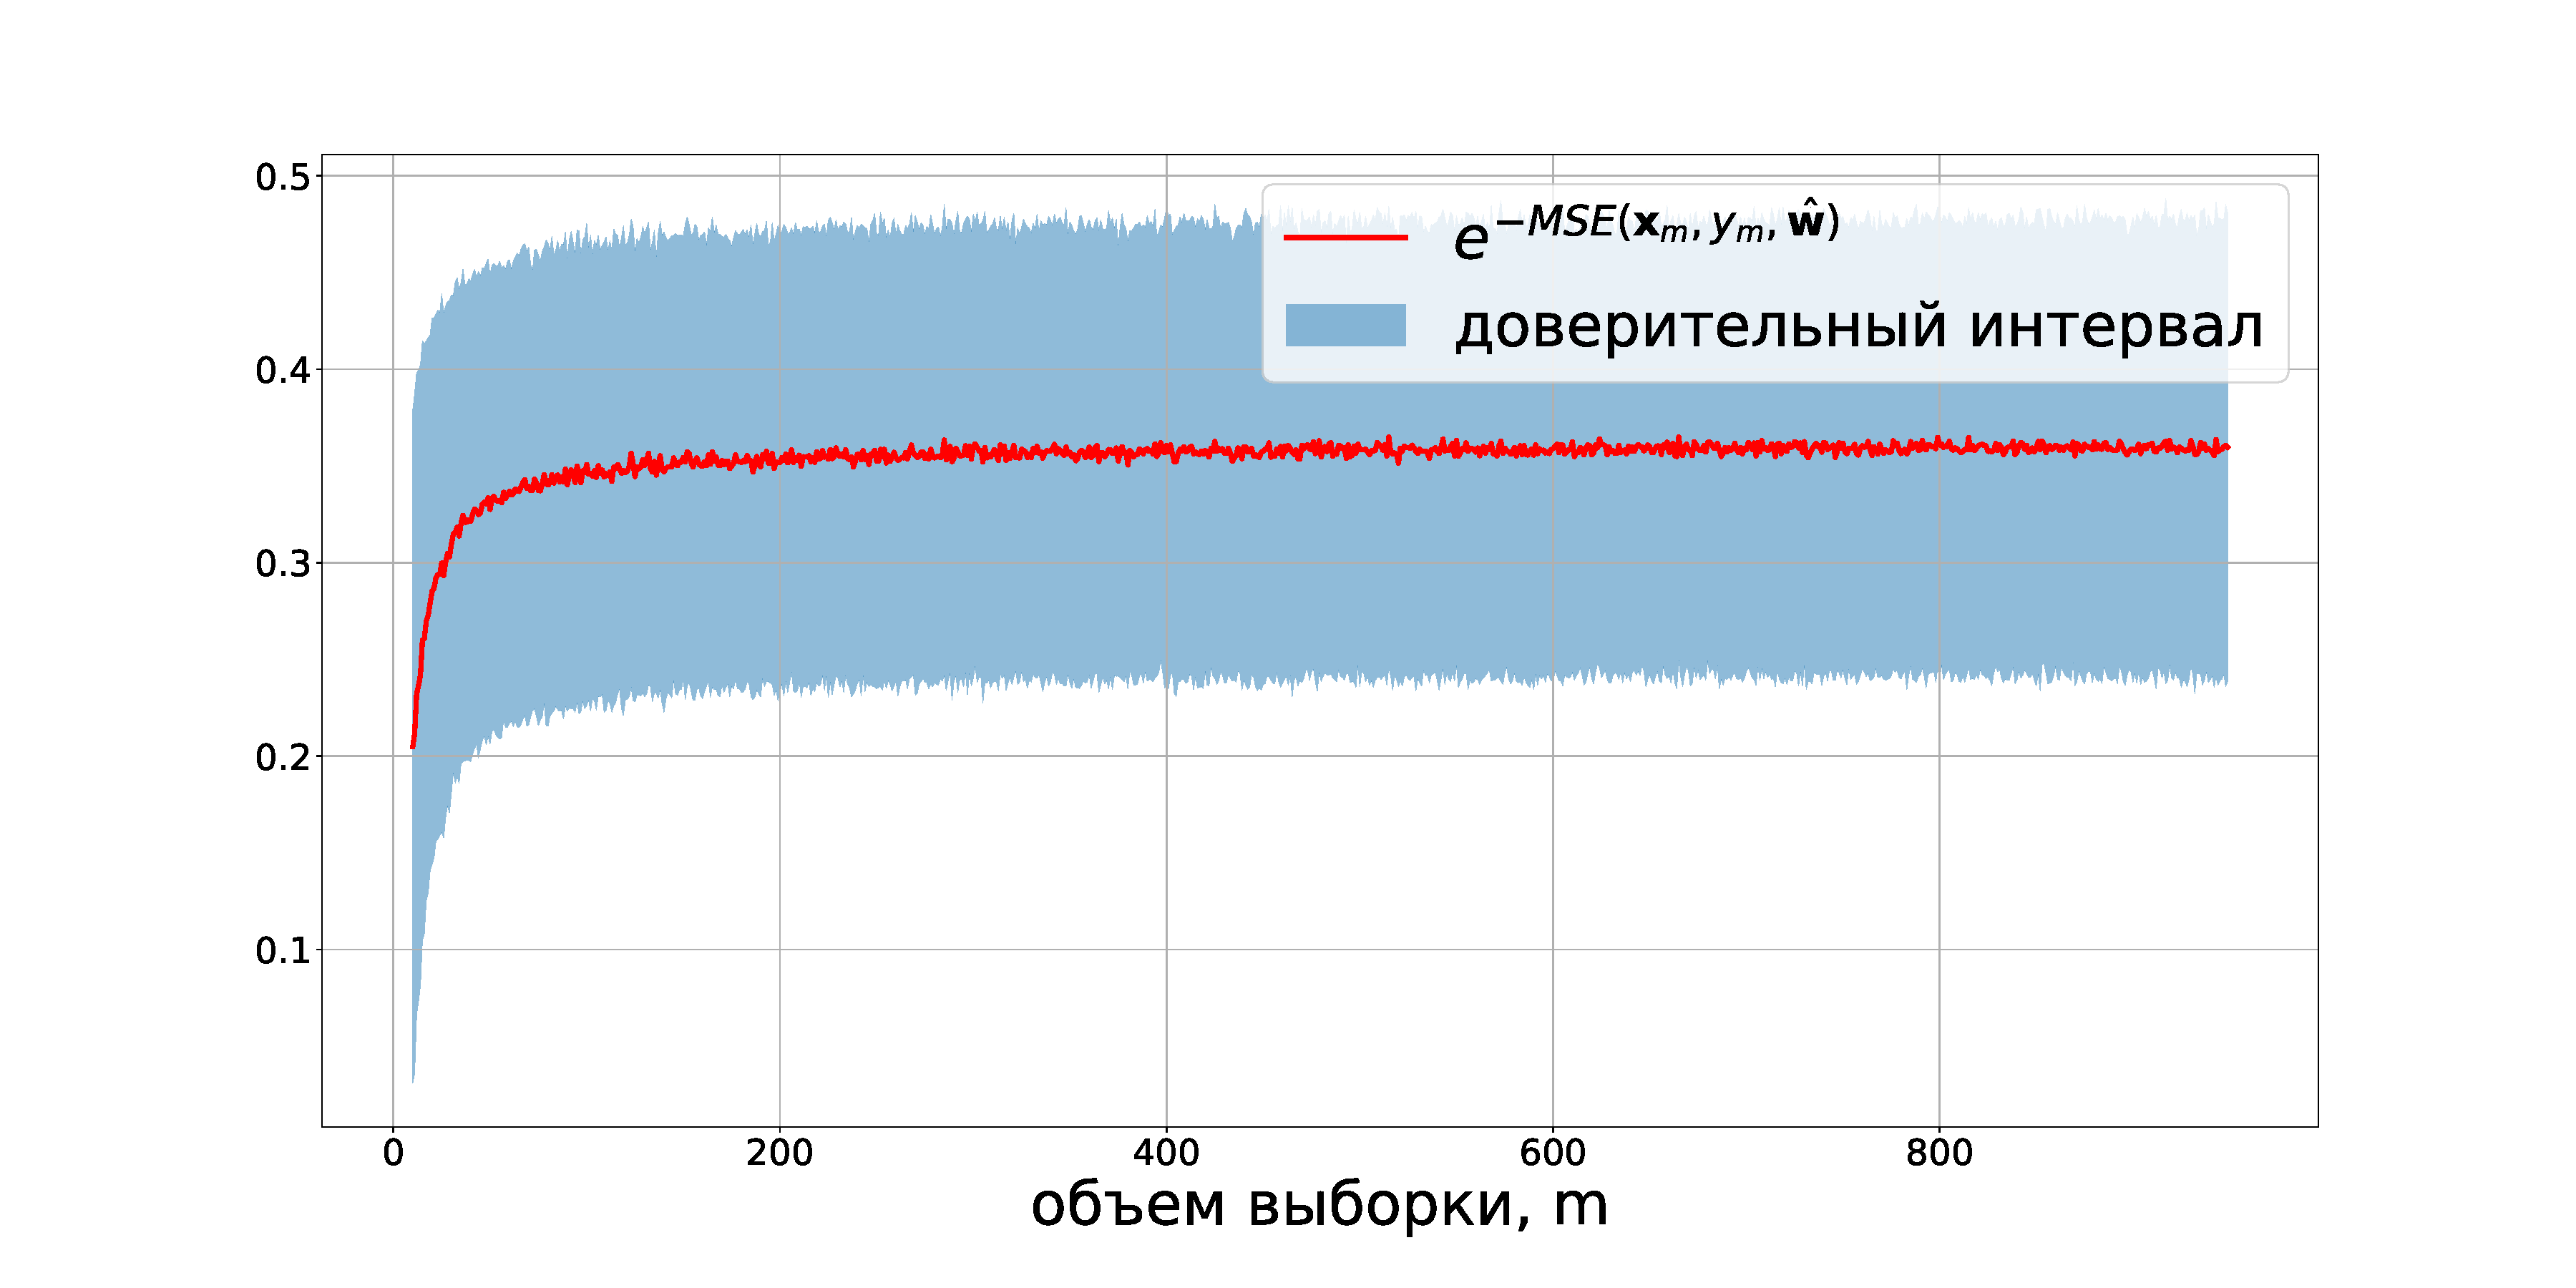
\includegraphics[width=1\textwidth]{../data/pics/synthetic_S.pdf}
\caption{Зависимость значения функции ошибки от объема выборки}
\label{fig1}
\end{figure}

$\newline$
$\newline$
$\newline$
$\newline$
$\newline$
$\newline$
$\newline$
$\newline$
$\newline$
$\newline$
$\newline$
$\newline$
$\newline$
$\newline$
$\newline$
$\newline$

\subsection{Аппроксимация $\hat{l}(m, n)$}

Пусть $\mathbf{X} = [\chi_1, ..., \chi_n]$ --- набор векторов-столбцов. Построим зависимость $\hat{l}(m, n)$ для различных конфигураций выборок:

\begin{enumerate}
	\item Адекватная случайная выборка ($m = 600, n = 10$): 
$$ 
\chi_i \sim U(5, 6), ~ \mathbf{w} \sim U(\mathbf{0}, \mathbf{1}), ~ y = \mathbf{w}^{\top}\mathbf{X} + \varepsilon,
$$
где $\varepsilon \sim \mathcal{N}(0, 0.1)$.
	\item Адекватная скоррелированная выборка ($m = 600, n = 10$):
$$
\chi_1, ..., \chi_3 \sim \mathcal{N}(1, 1),~ \chi_4, ..., \chi_6 \sim \chi_0 + \varepsilon, ~\chi_7, ..., \chi_{10} \sim \chi_1 + \varepsilon,
$$
$$
	y = 0.3\chi_1 + 0.7\chi_2 + \varepsilon,
$$
где $\varepsilon \sim \mathcal{N}(0, 0.1)$,
	\item Адекватная ортогональная выборка ($m = 600, n = 10$):
$$
	\{\chi_i \in \mathbb{R}^{m}\}_{i=1}^{n}  \text{ --- ортогональный набор}, ~\mathbf{w} \sim \mathcal{N}(\mathbf{1}, I), ~y = \mathbf{w}^{\top}\mathbf{X} + \varepsilon,
$$
где $\varepsilon \sim \mathcal{N}(0, 0.1)$.
	\item Адекватная избыточная выборка:
$$
	\chi_i \sim \mathcal{N}(1, 1), 
$$
$$
	w_i \sim U(1, 1), ~i \leq 5, 
$$
$$
	w_i = 0, ~i > 5,
$$
$$
	y = \mathbf{w}^{\top}\mathbf{X} + \varepsilon,
$$
где $\varepsilon \sim \mathcal{N}(0, 0.1)$
	\item Неадекватная скоррелированная выборка:
$$
	y \perp \chi_0 \in \mathbb{R}^m, ~\chi_i = \chi_0 + \mathcal{N}(0, 0.1).
$$
\end{enumerate}

На рис. 2 представлена функция $\hat{l}(m, n)$, посчитанная  с помощью бутстрепа в варианте 1.

$\newline$
$\newline$

\begin{figure}[h!t]\center
\centering\begin{tabular}{@{}c@{ }c@{ }c@{}}
\subfloat[Адекватная случайная выборка]{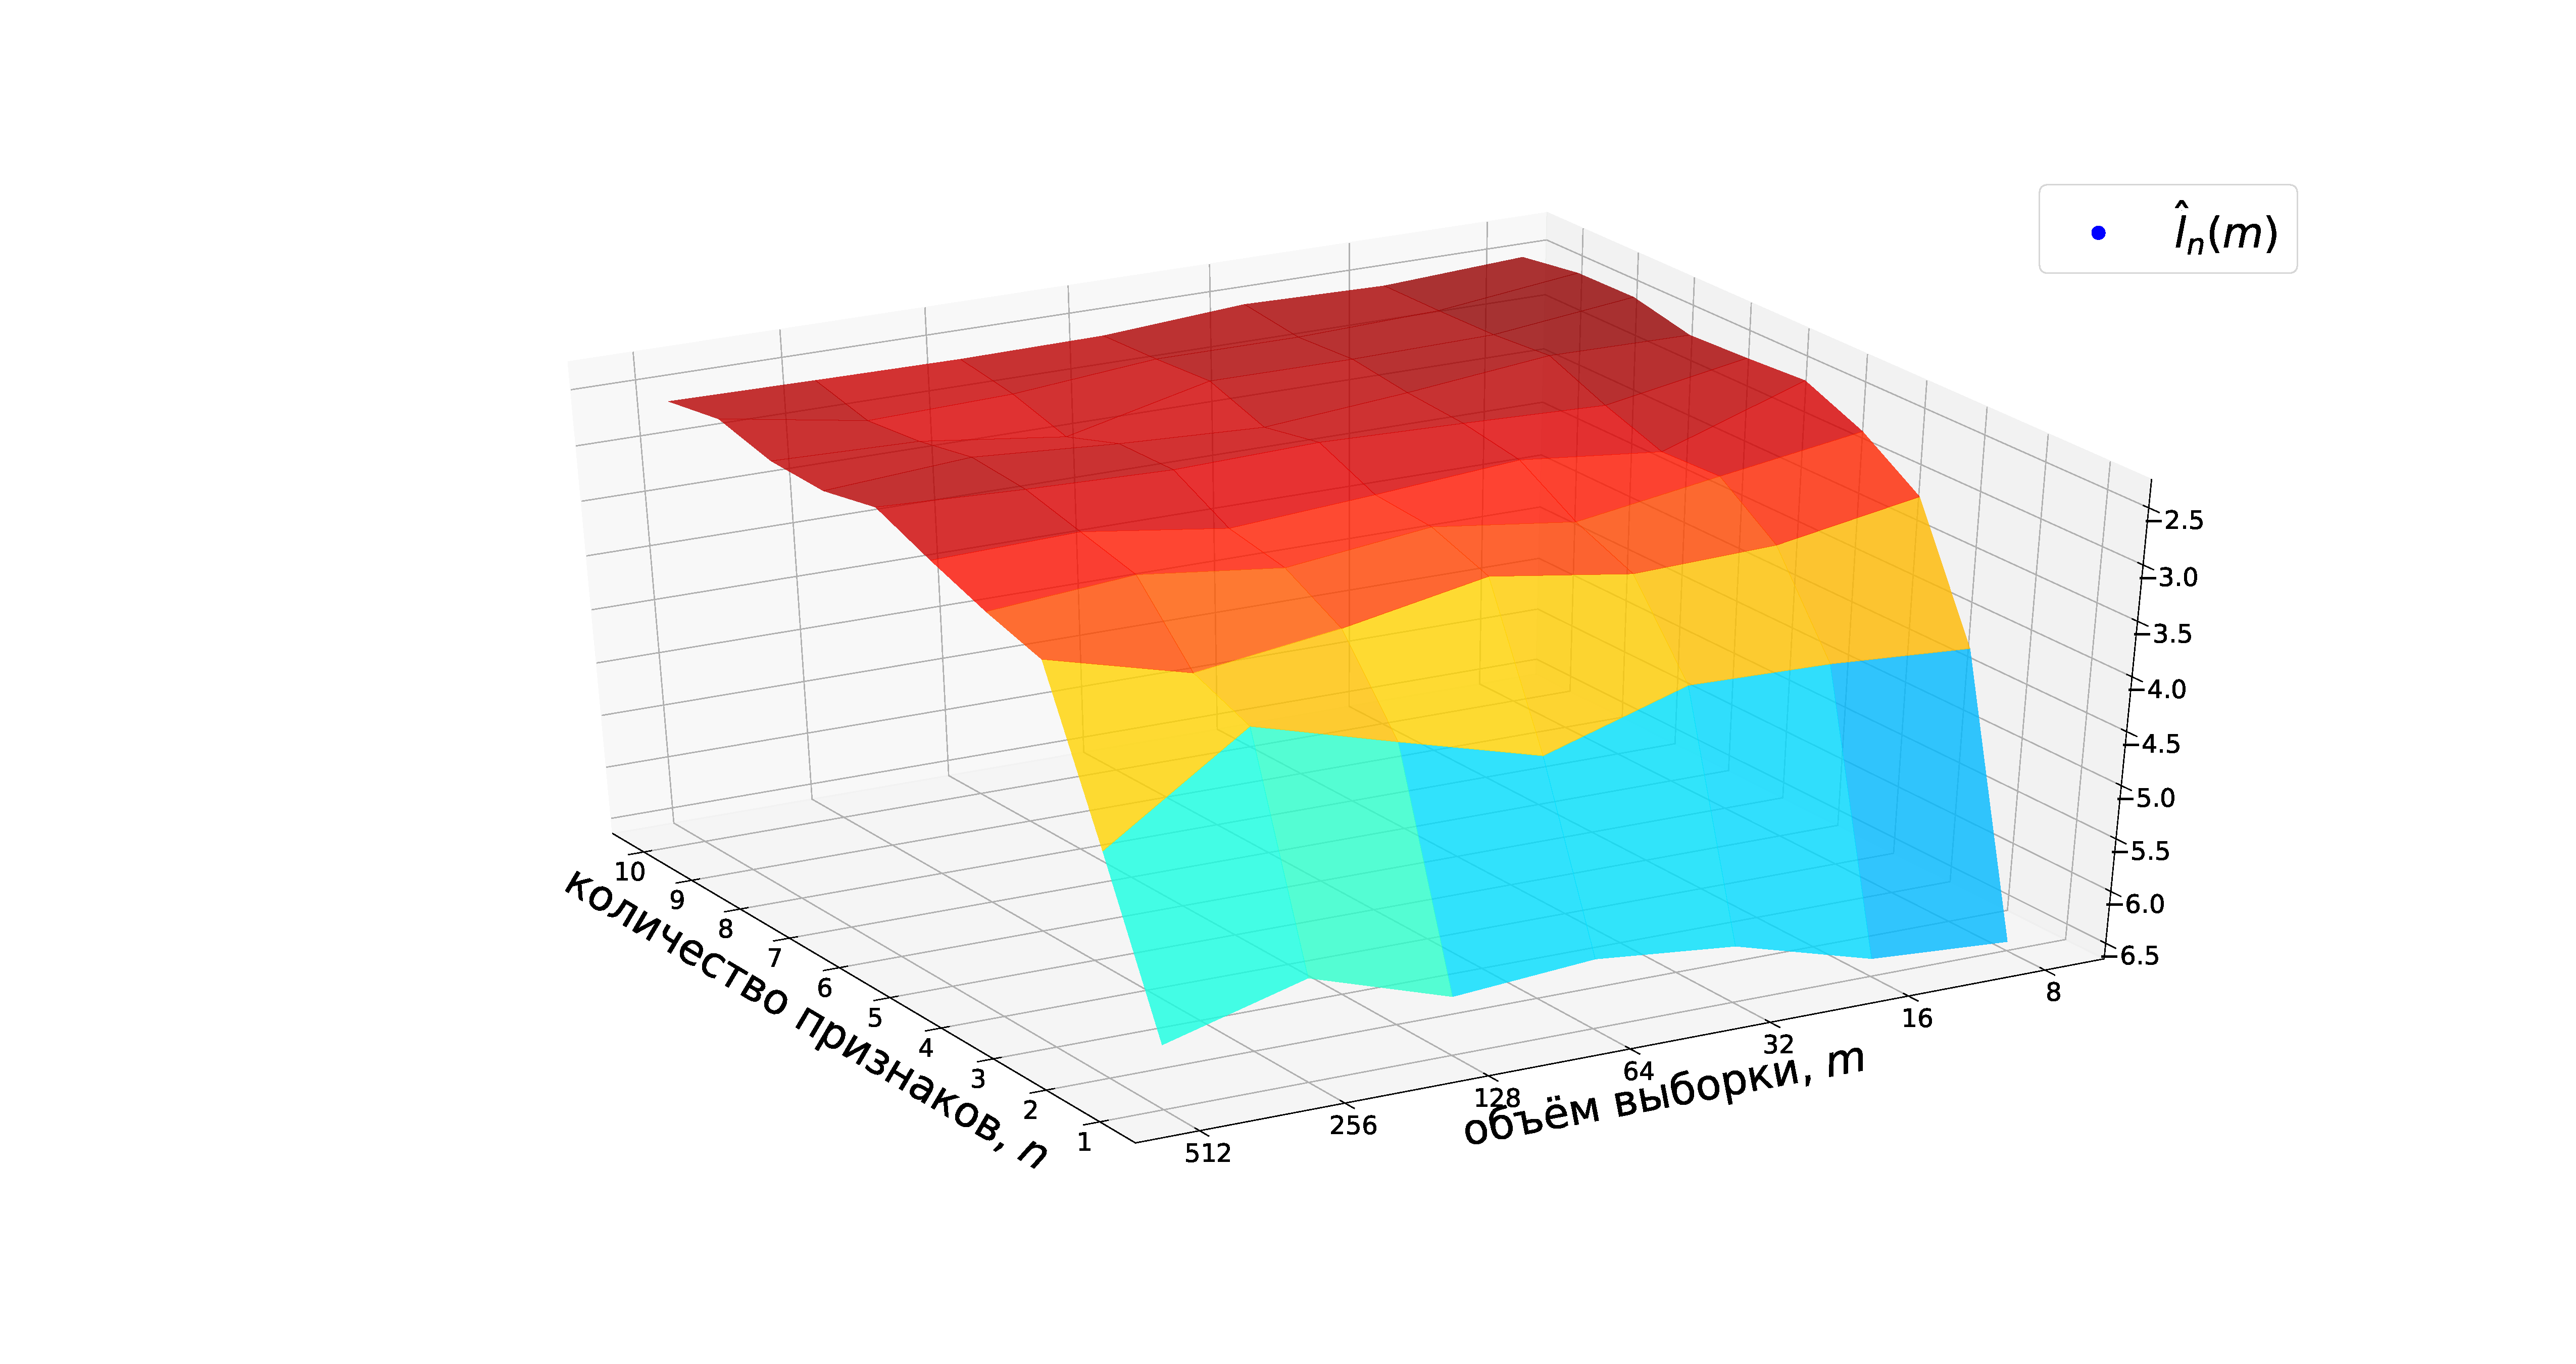
\includegraphics[width=0.5\textwidth]{../data/pics/theoretical_adequate_random_sample_llh.pdf}}&
\subfloat[Адекватная скоррелированная выборка]{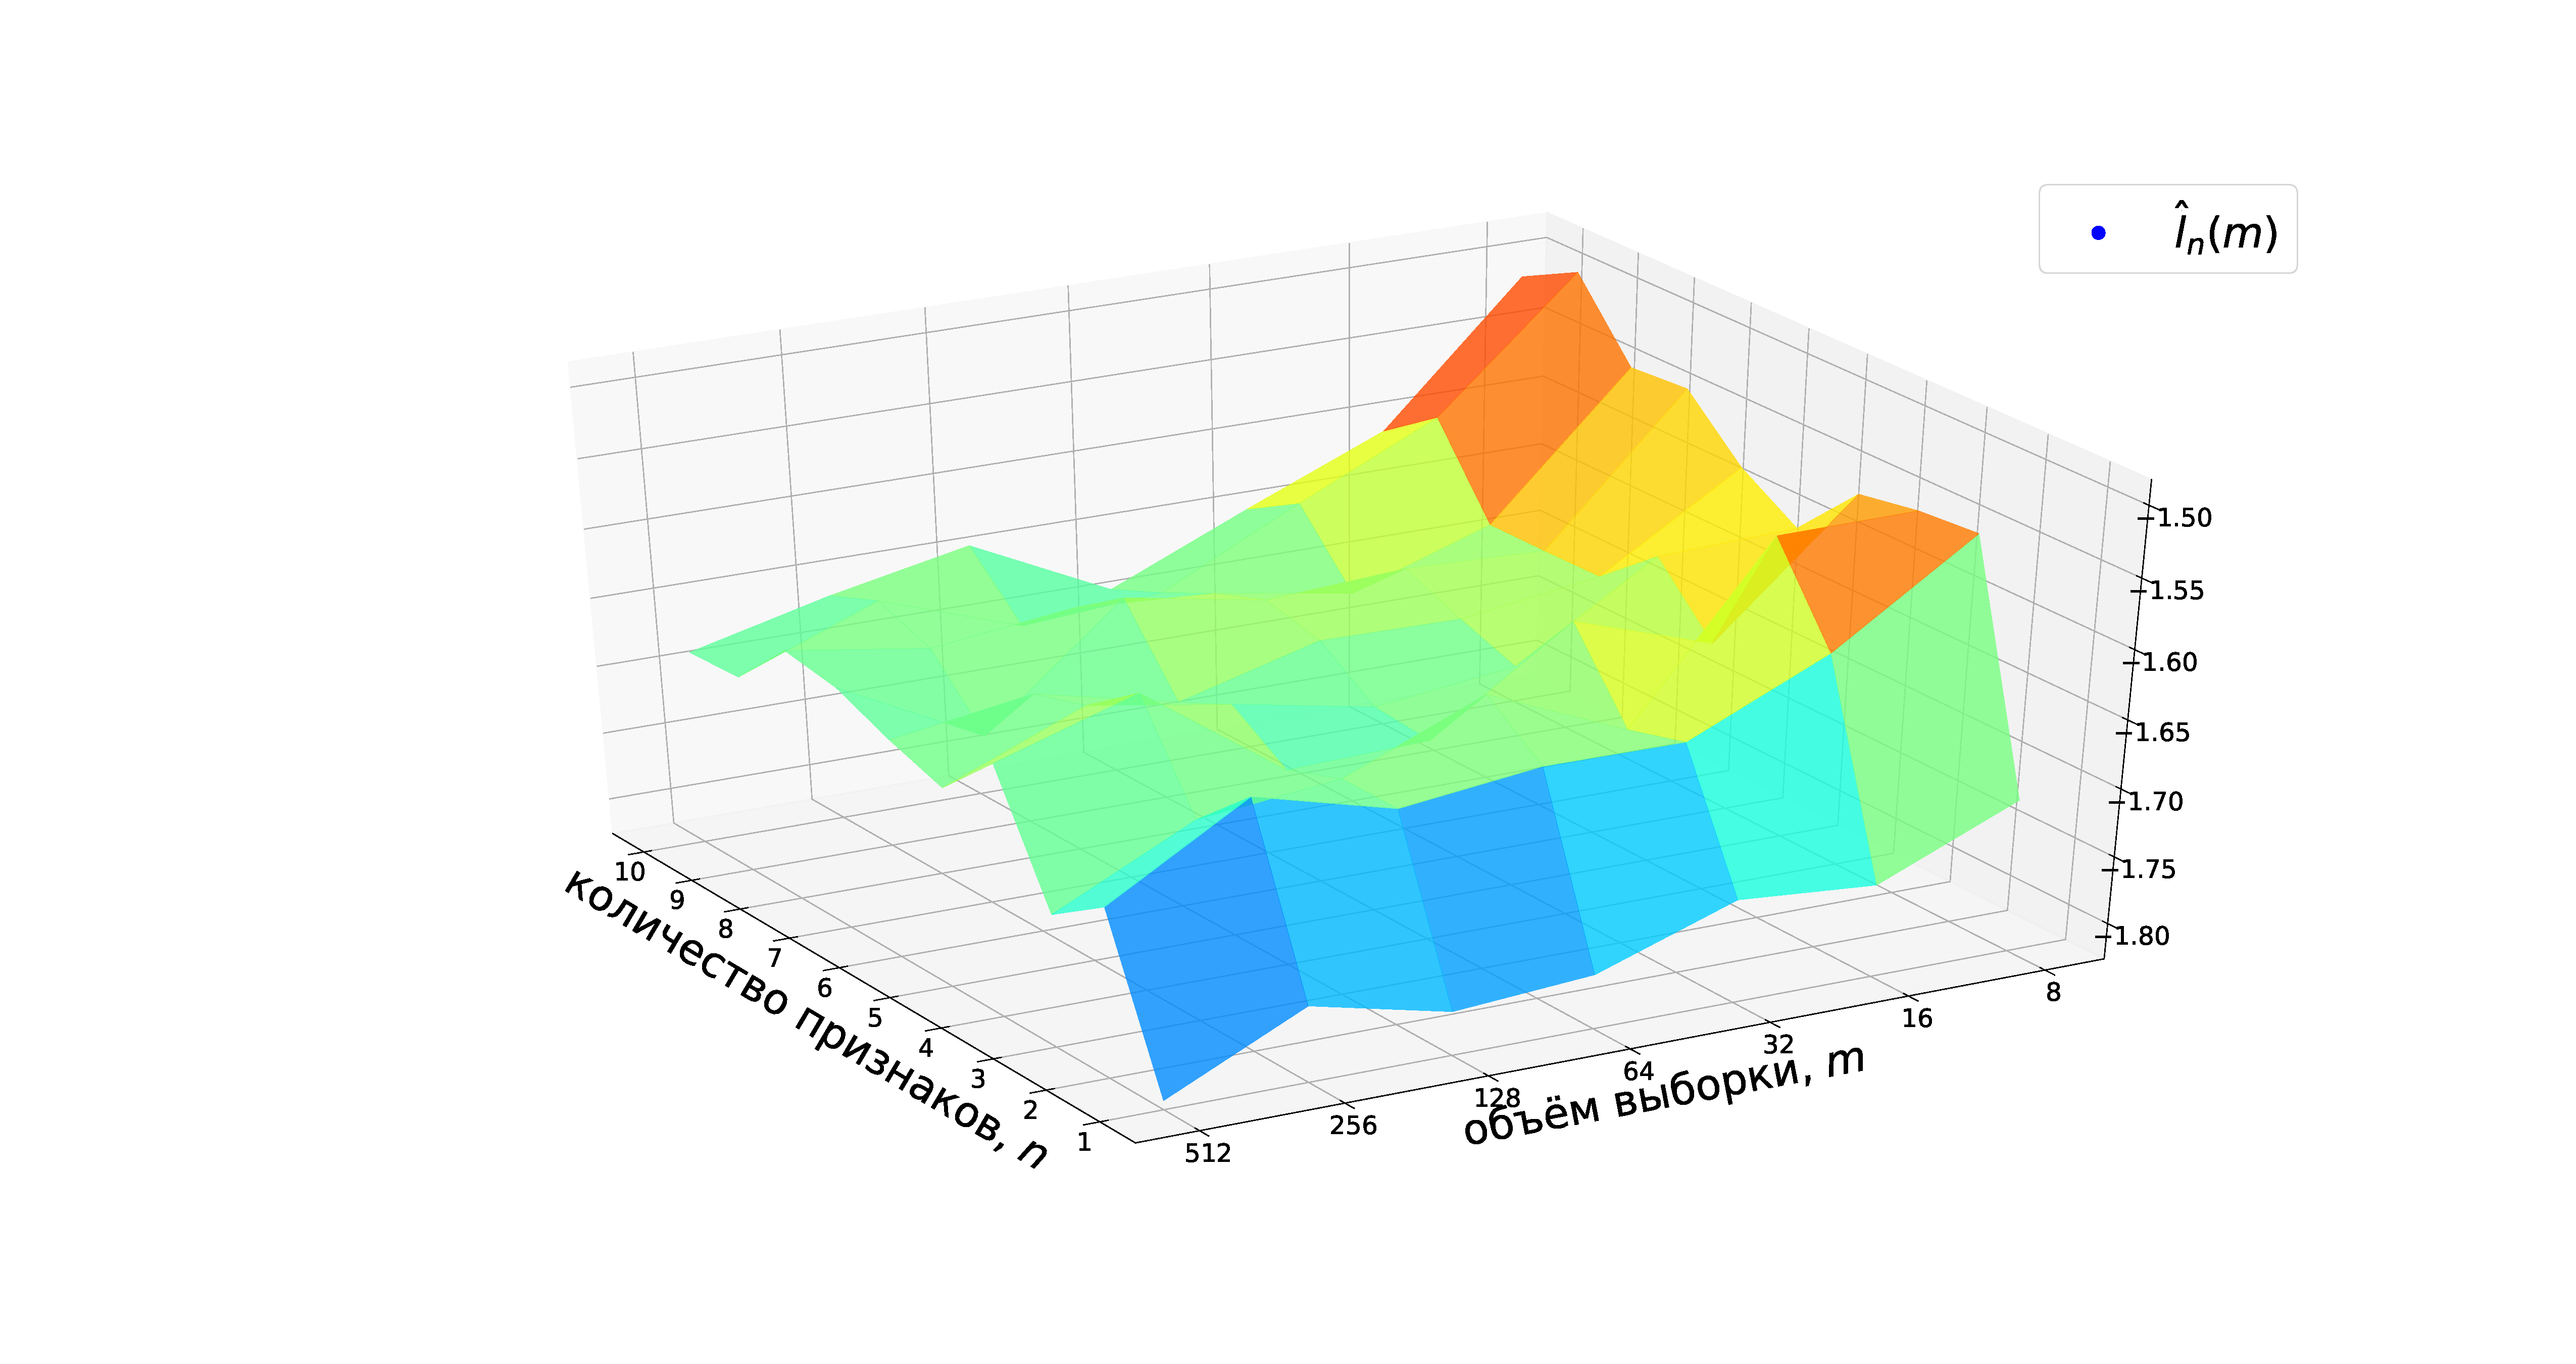
\includegraphics[width=0.5\textwidth]{../data/pics/theoretical_adequate_correlated_sample_llh.pdf}}\\
\subfloat[Адекватная ортогональная выборка]{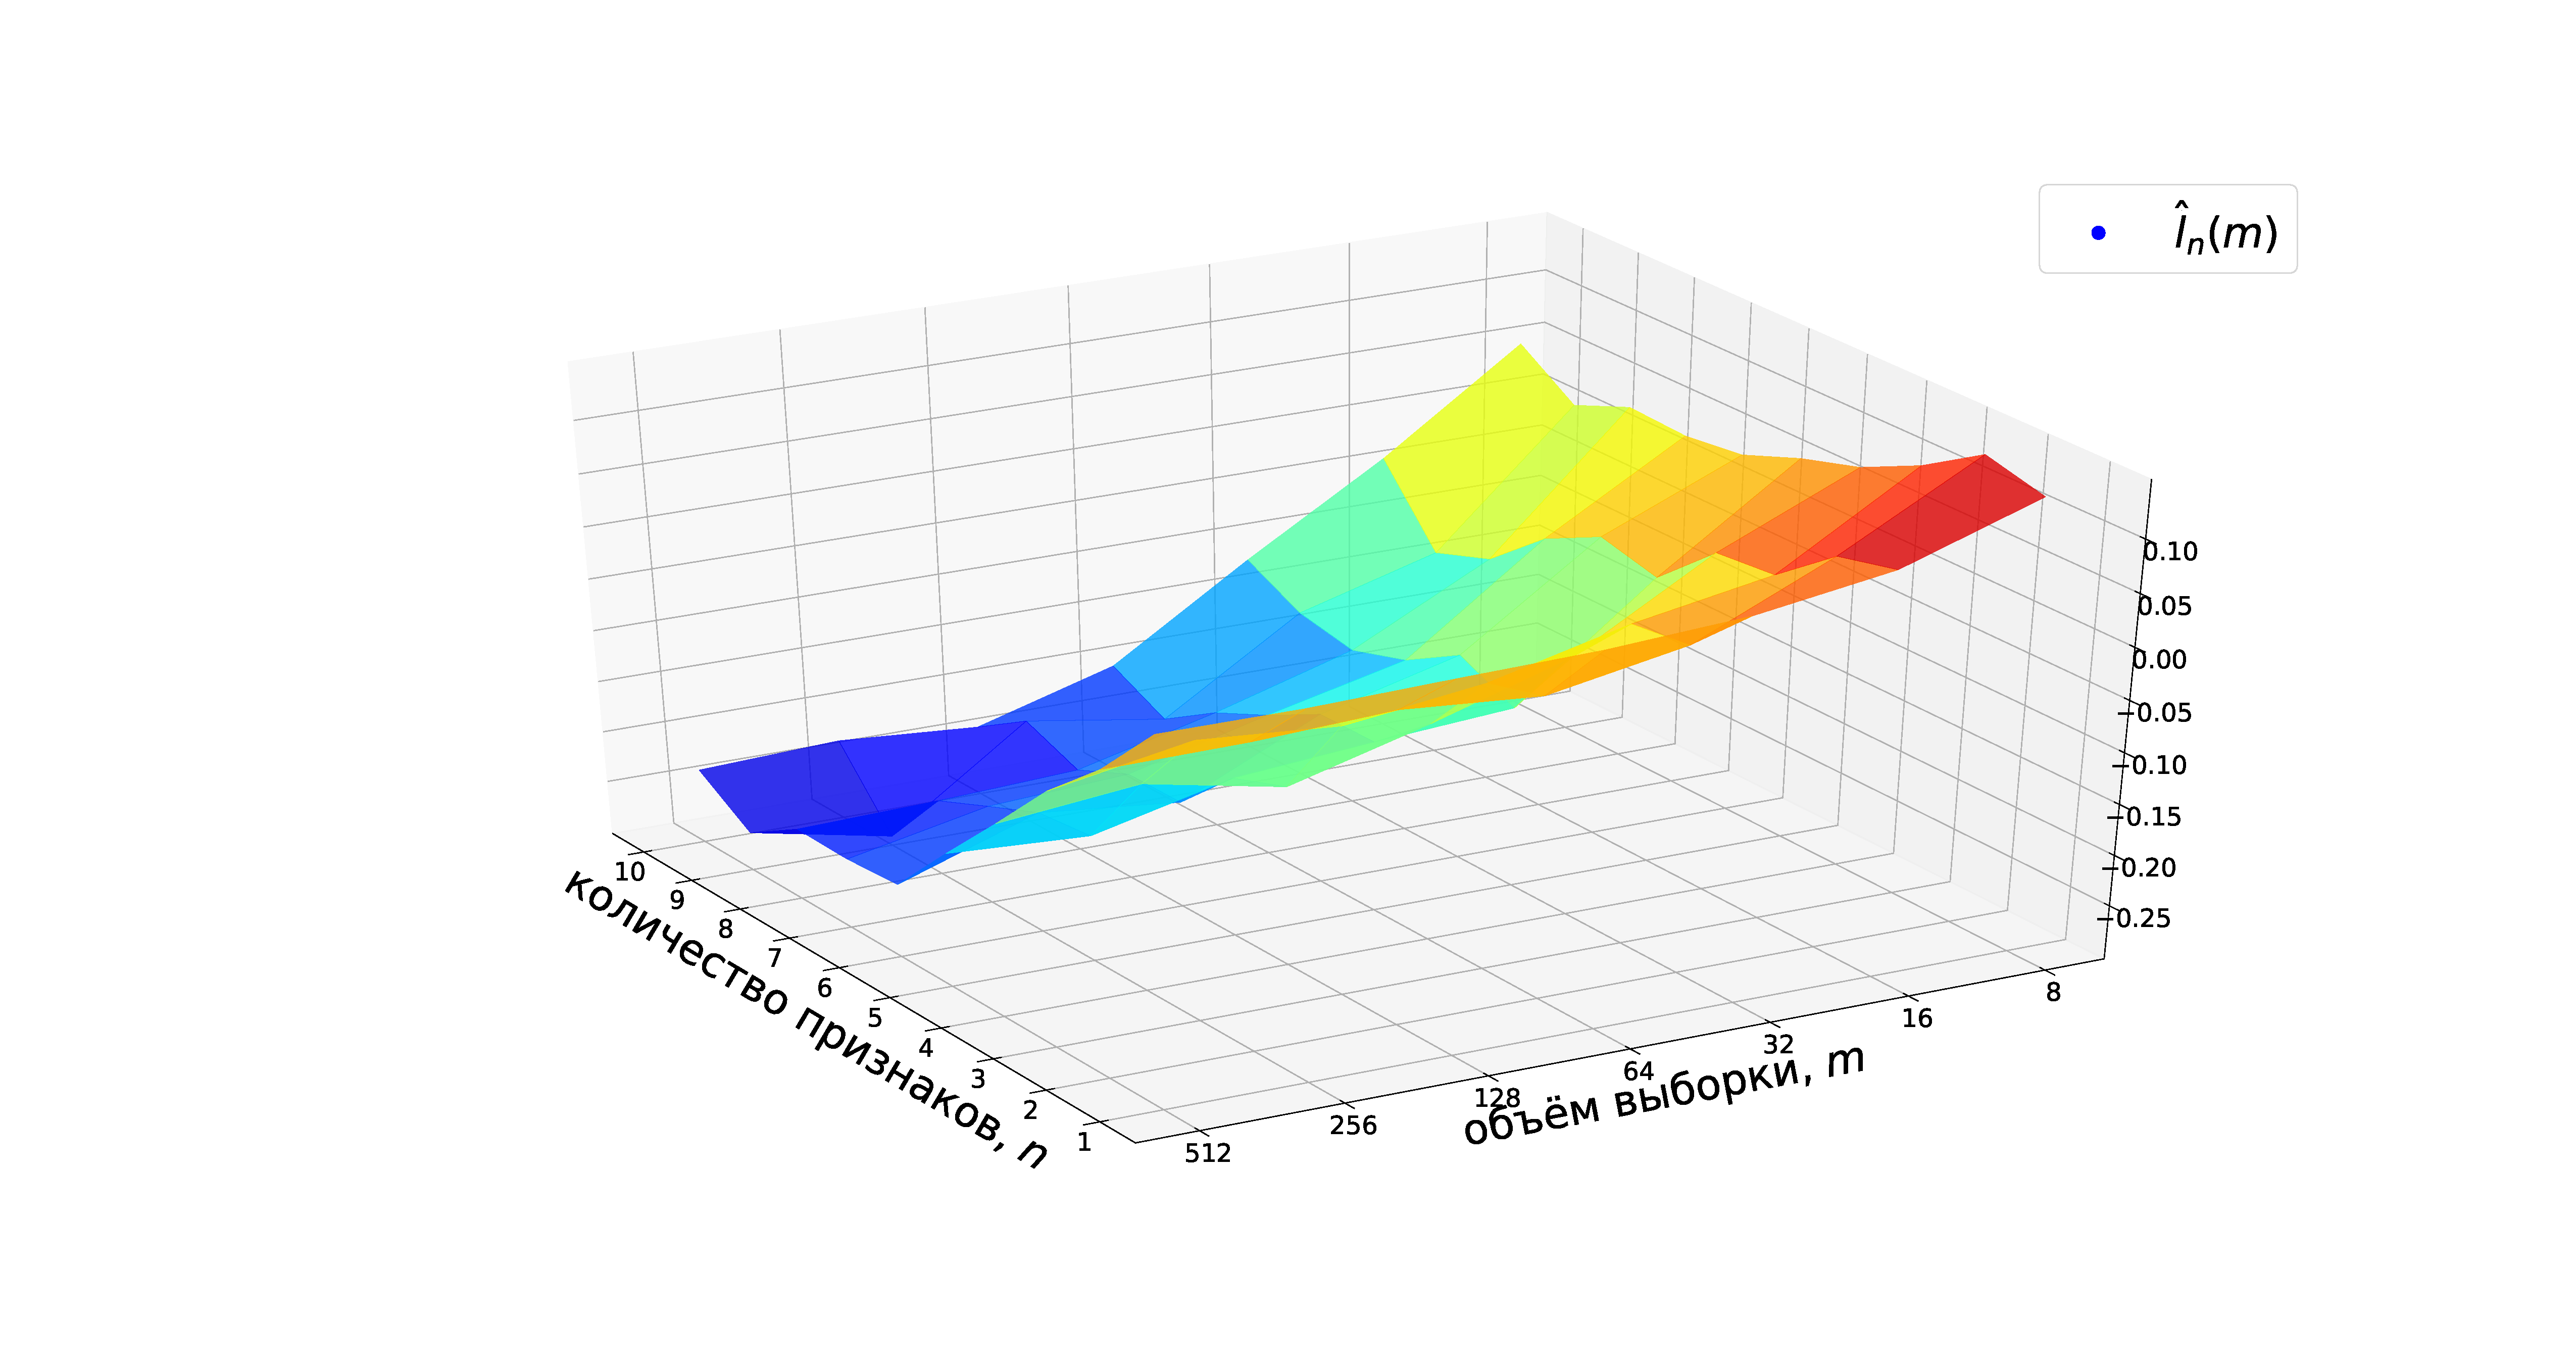
\includegraphics[width=0.5\textwidth]{../data/pics/theoretical_adequate_orthogonal_sample_llh.pdf}}&
\subfloat[Адекватная избыточная выборка]{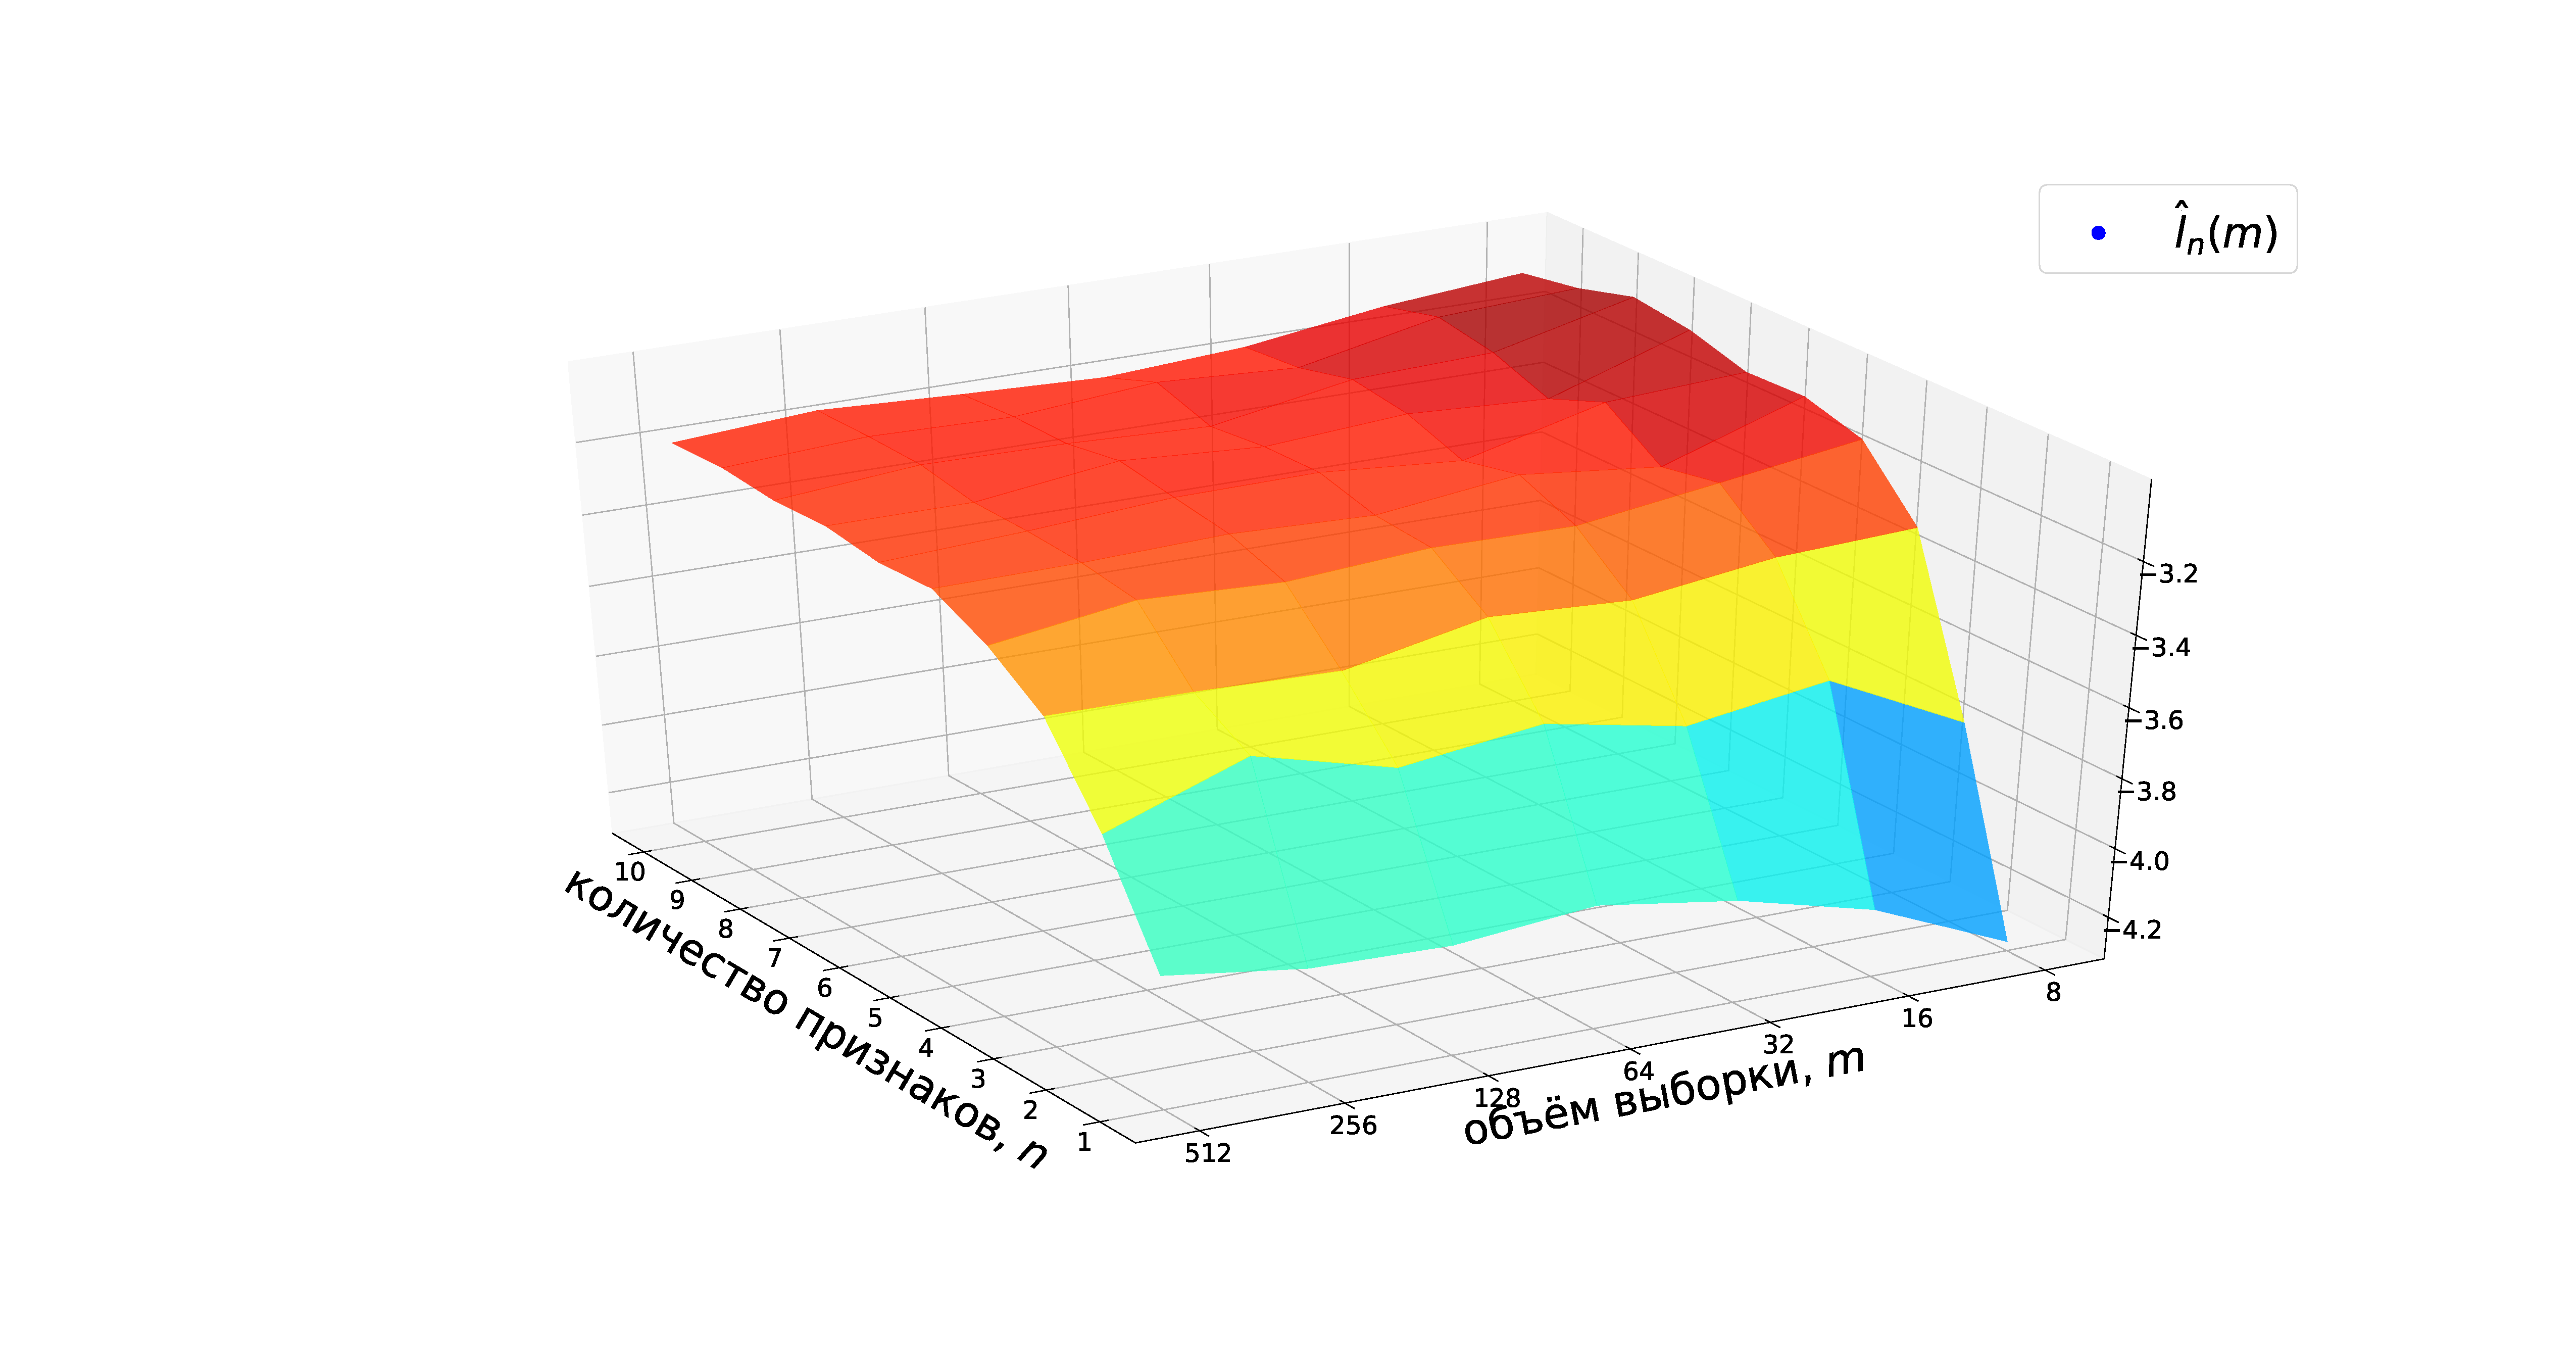
\includegraphics[width=0.5\textwidth]{../data/pics/theoretical_adequate_redundant_sample_llh.pdf}}\\
\subfloat[Недекватная скоррелированная выборка]{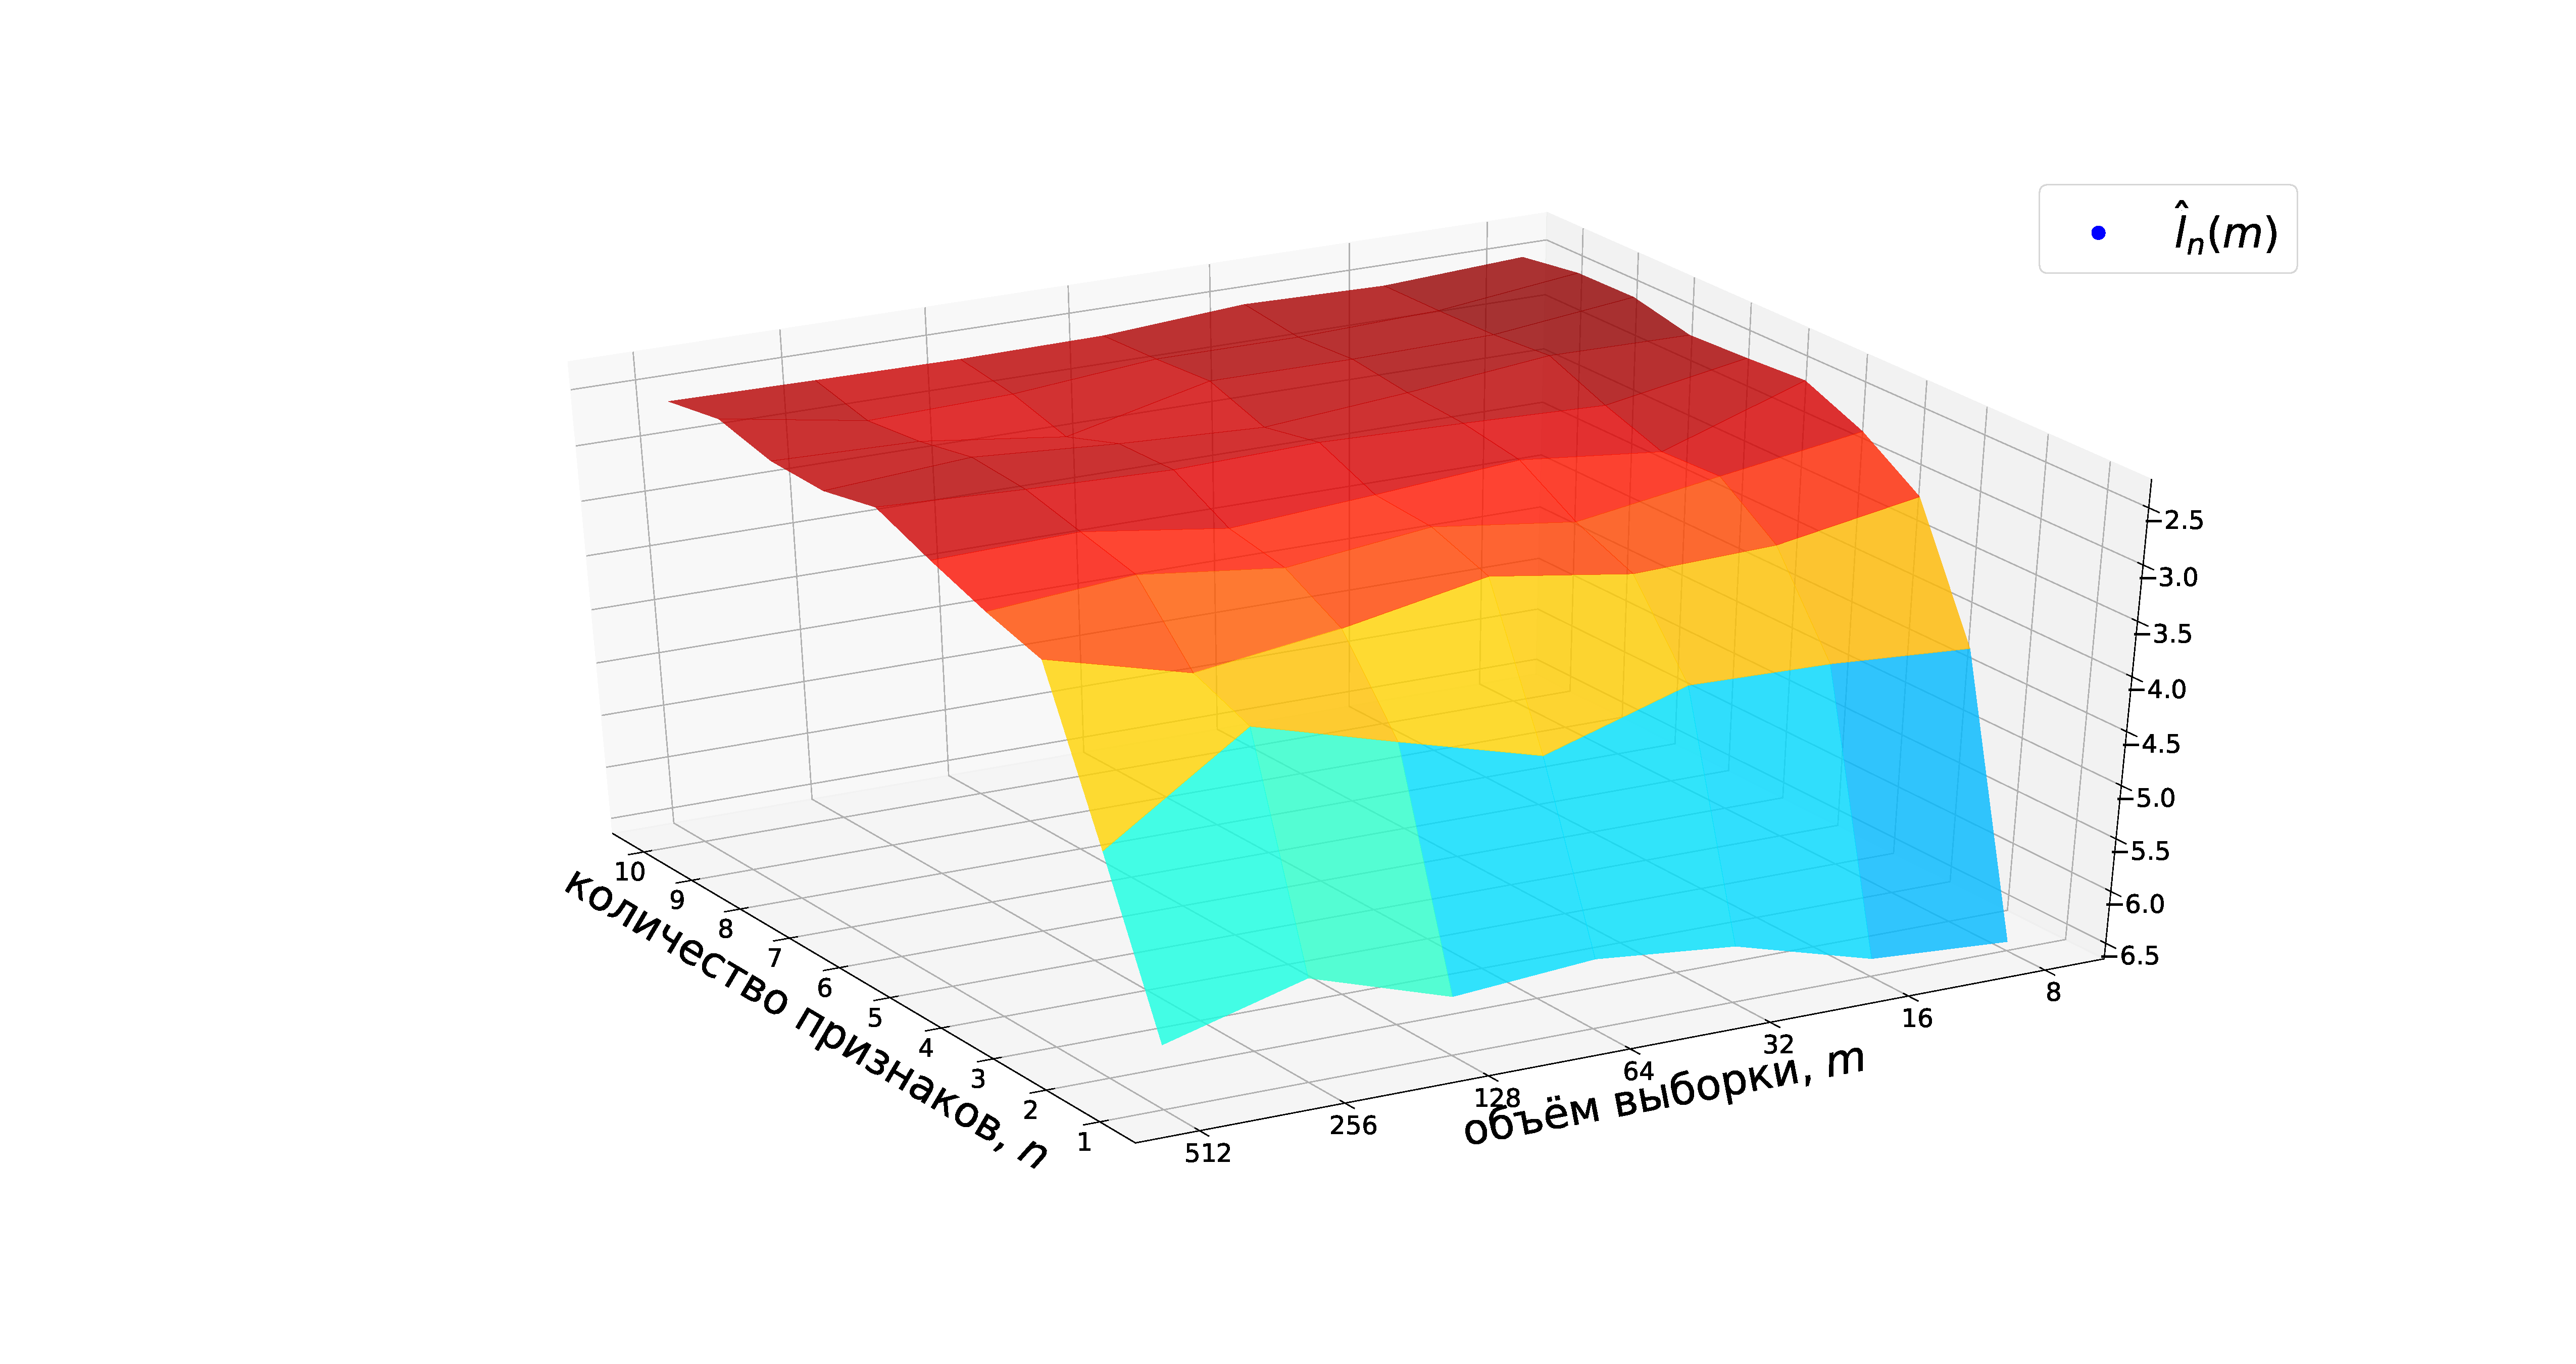
\includegraphics[width=0.5\textwidth]{../data/pics/theoretical_adequate_random_sample_llh.pdf}}&\\
\end{tabular}

\caption{Зависимость значения функции $\hat{l}(m, n)$ от объема выборки $m$ и количества параметров $n$}
\label{fig100}
\end{figure}

На рис. 3 представлена аппроксимация $\phi(p, \hat{A}(m, n), m, n) \sim \hat{l}(m, n)$ при $m_0 = 100$.

\begin{figure}[h!t]\center
\centering\begin{tabular}{@{}c@{ }c@{ }c@{}}
\textbf{Вариант 1} & \textbf{Вариант 2}\\
\subfloat[Адекватная случайная выборка]{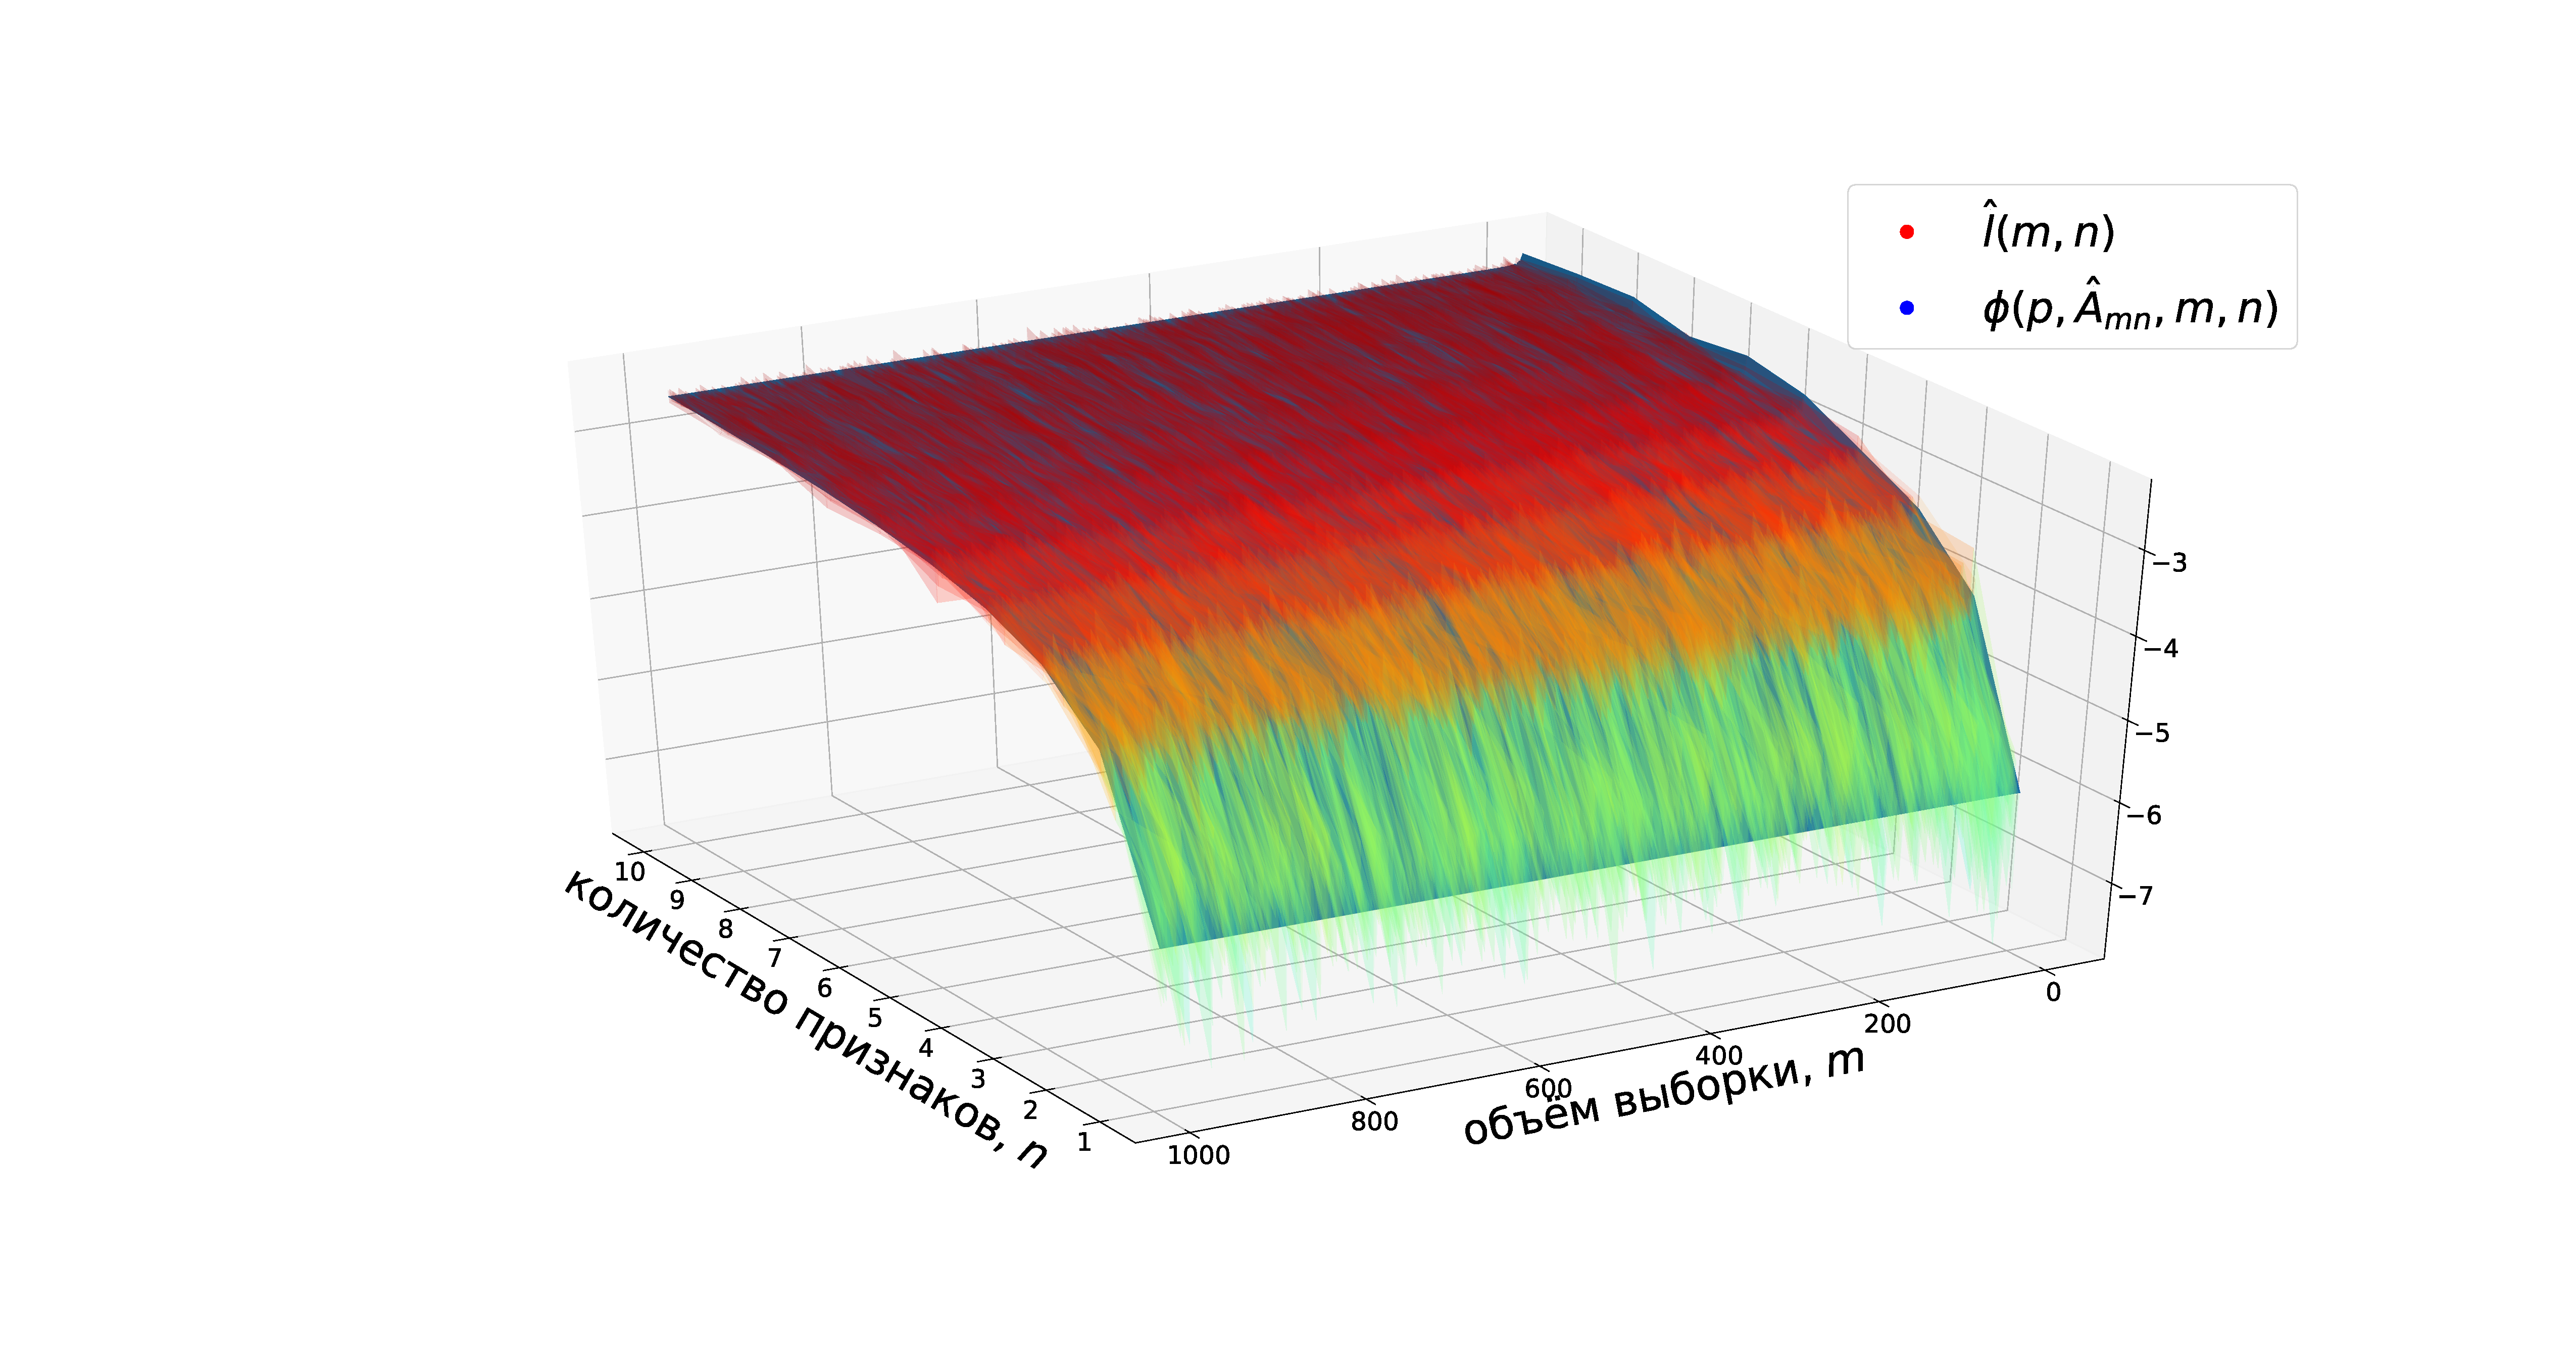
\includegraphics[width=0.5\textwidth]{../data/pics/theoretical_adequate_random_sample_llh_phi.pdf}}&
\subfloat[Адекватная случайная выборка]{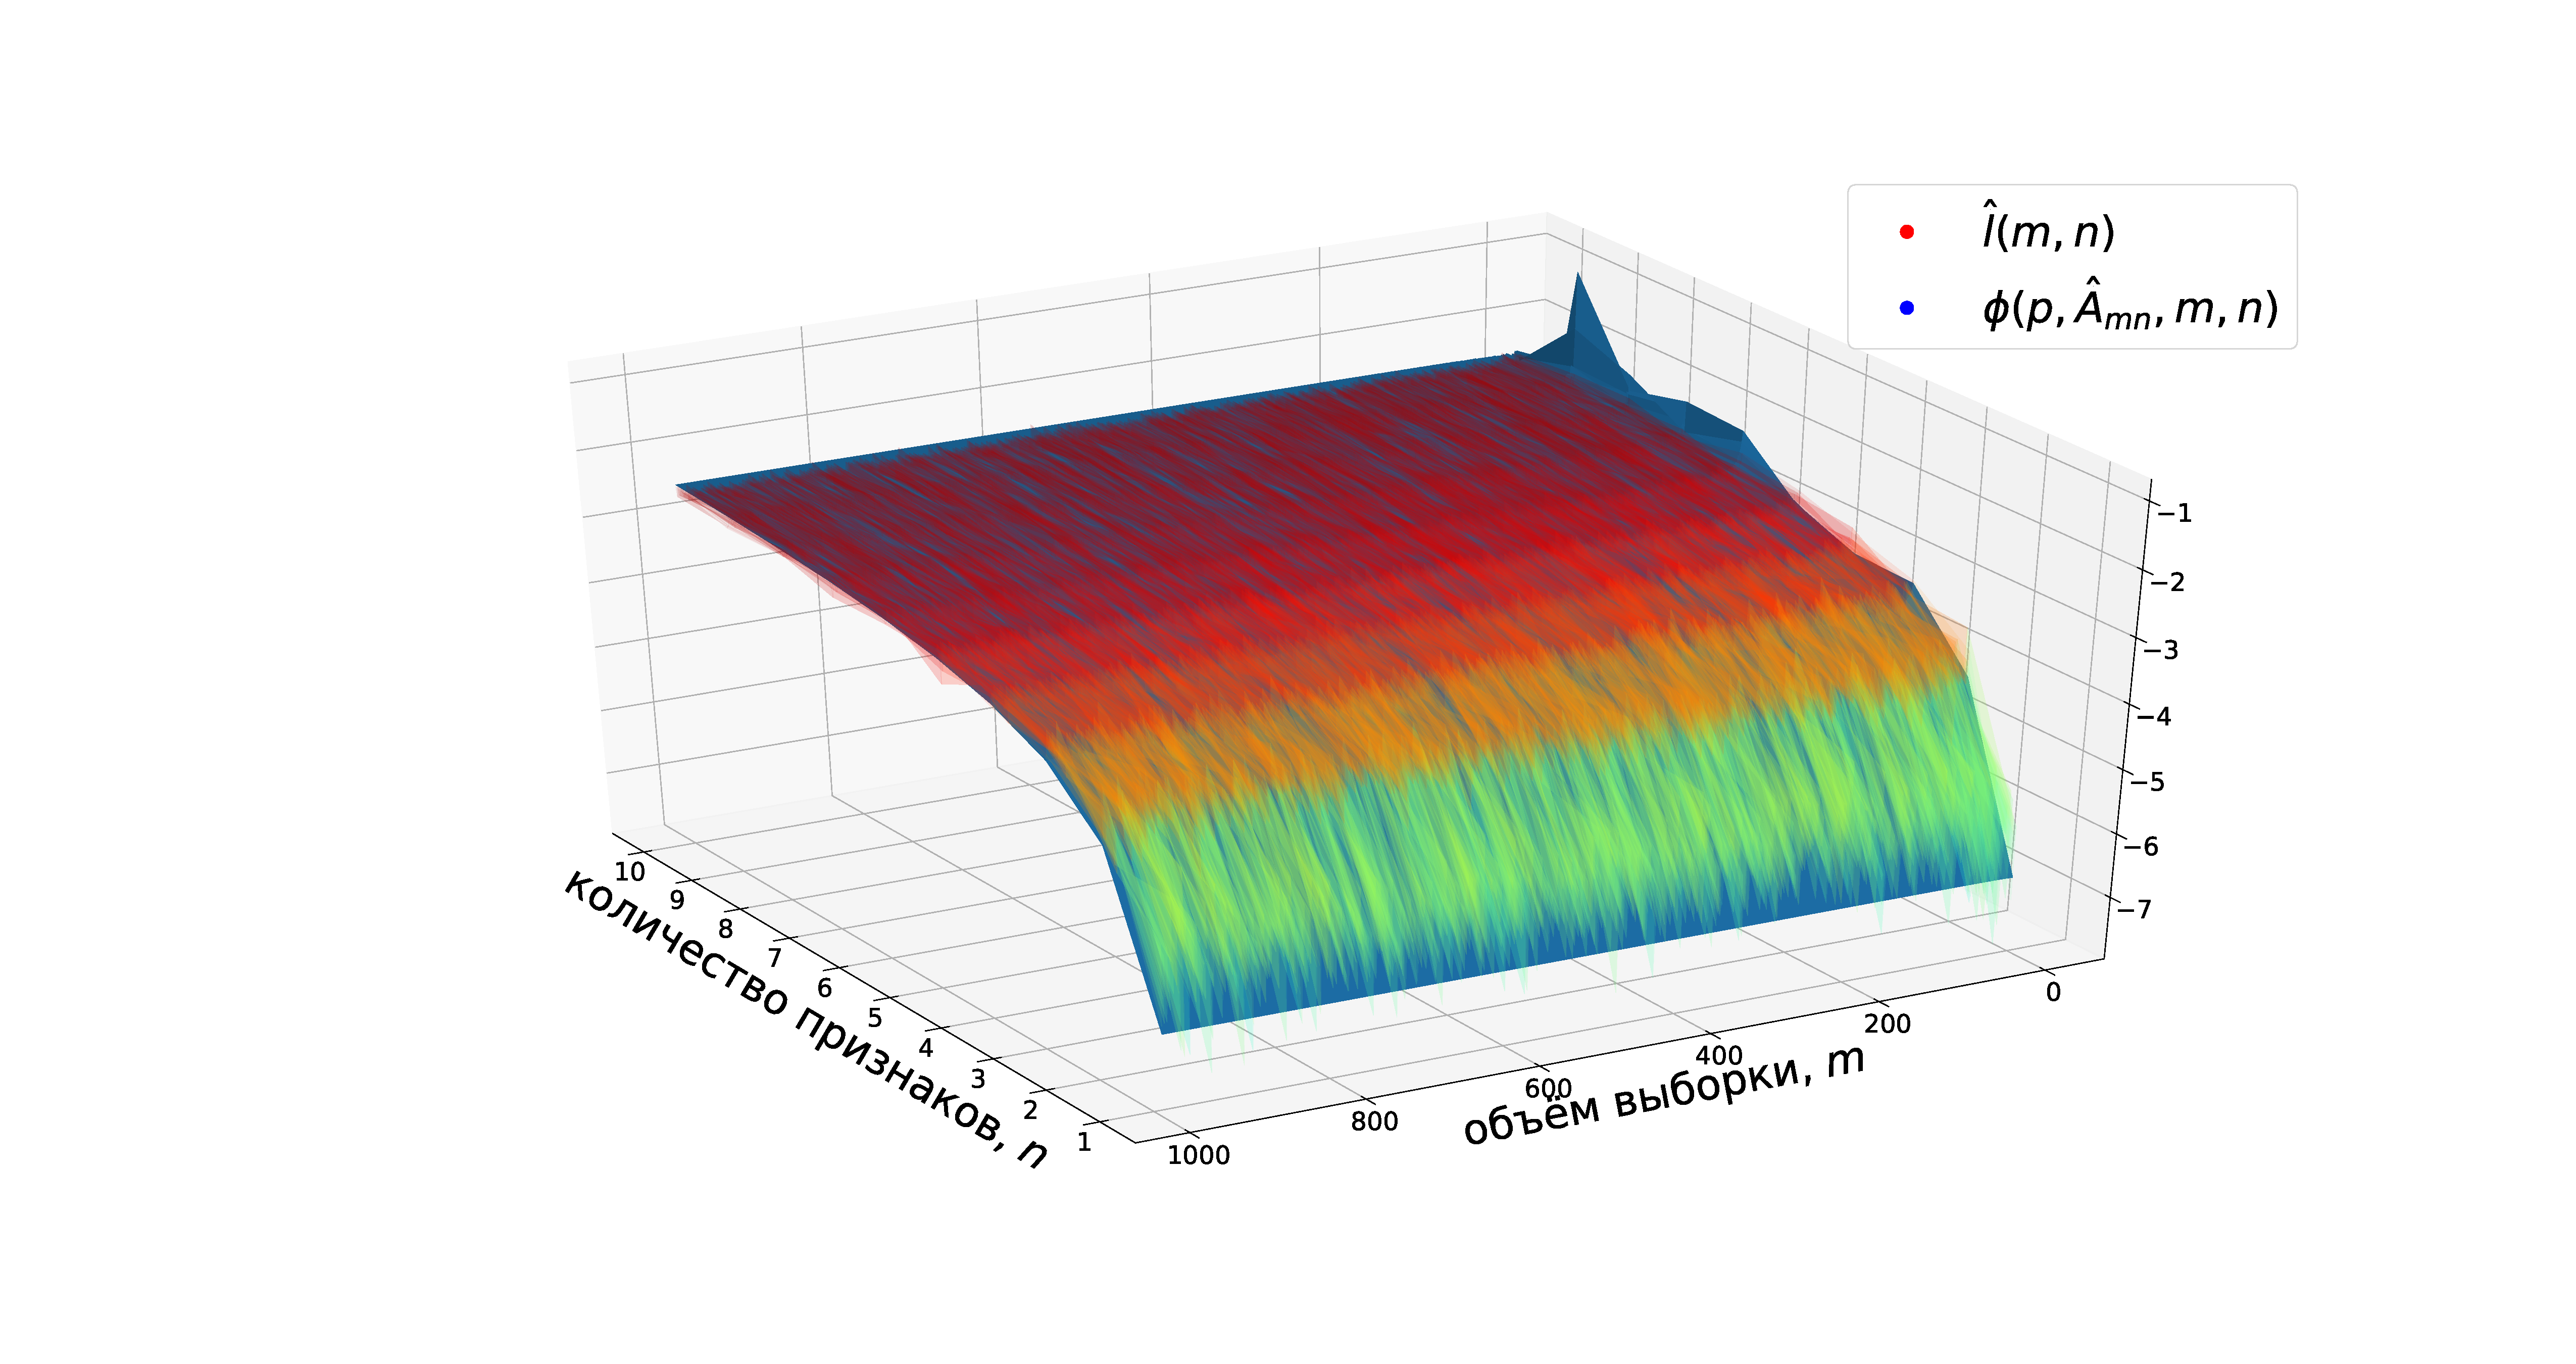
\includegraphics[width=0.5\textwidth]{../data/pics/exploitational_adequate_random_sample_llh_phi.pdf}}\\
\subfloat[Адекватная скоррелированная выборка]{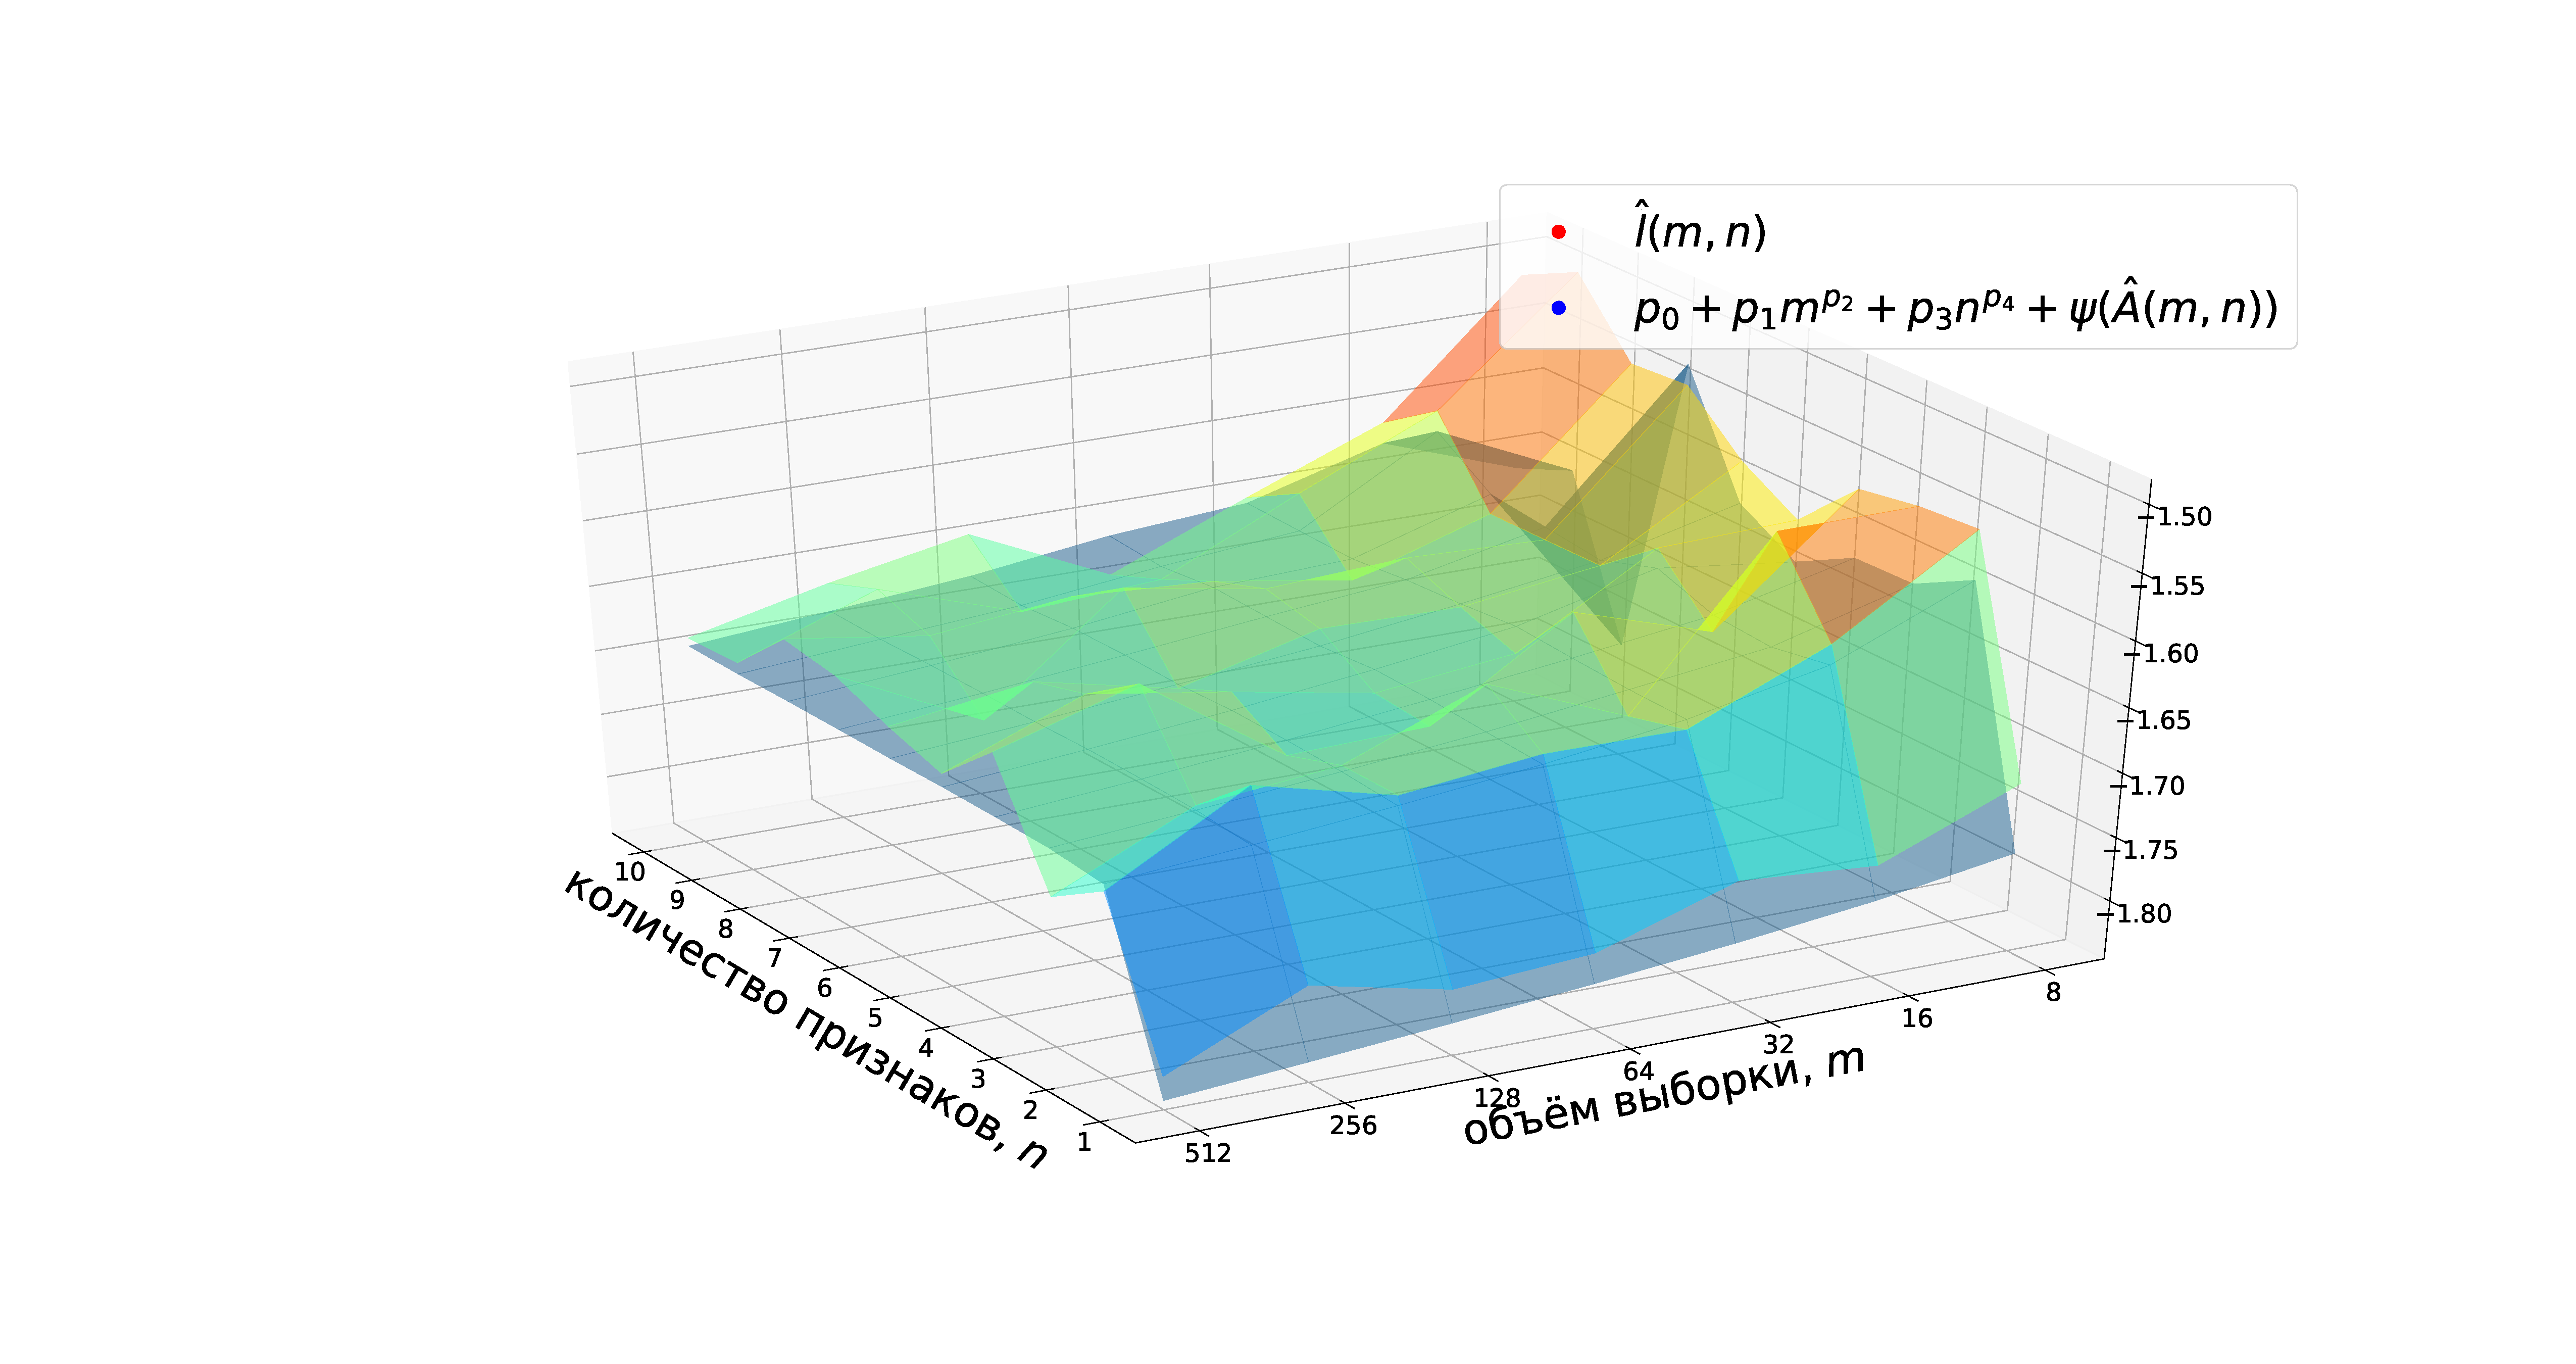
\includegraphics[width=0.5\textwidth]{../data/pics/theoretical_adequate_correlated_sample_llh_phi.pdf}}&
\subfloat[Адекватная скоррелированная выборка]{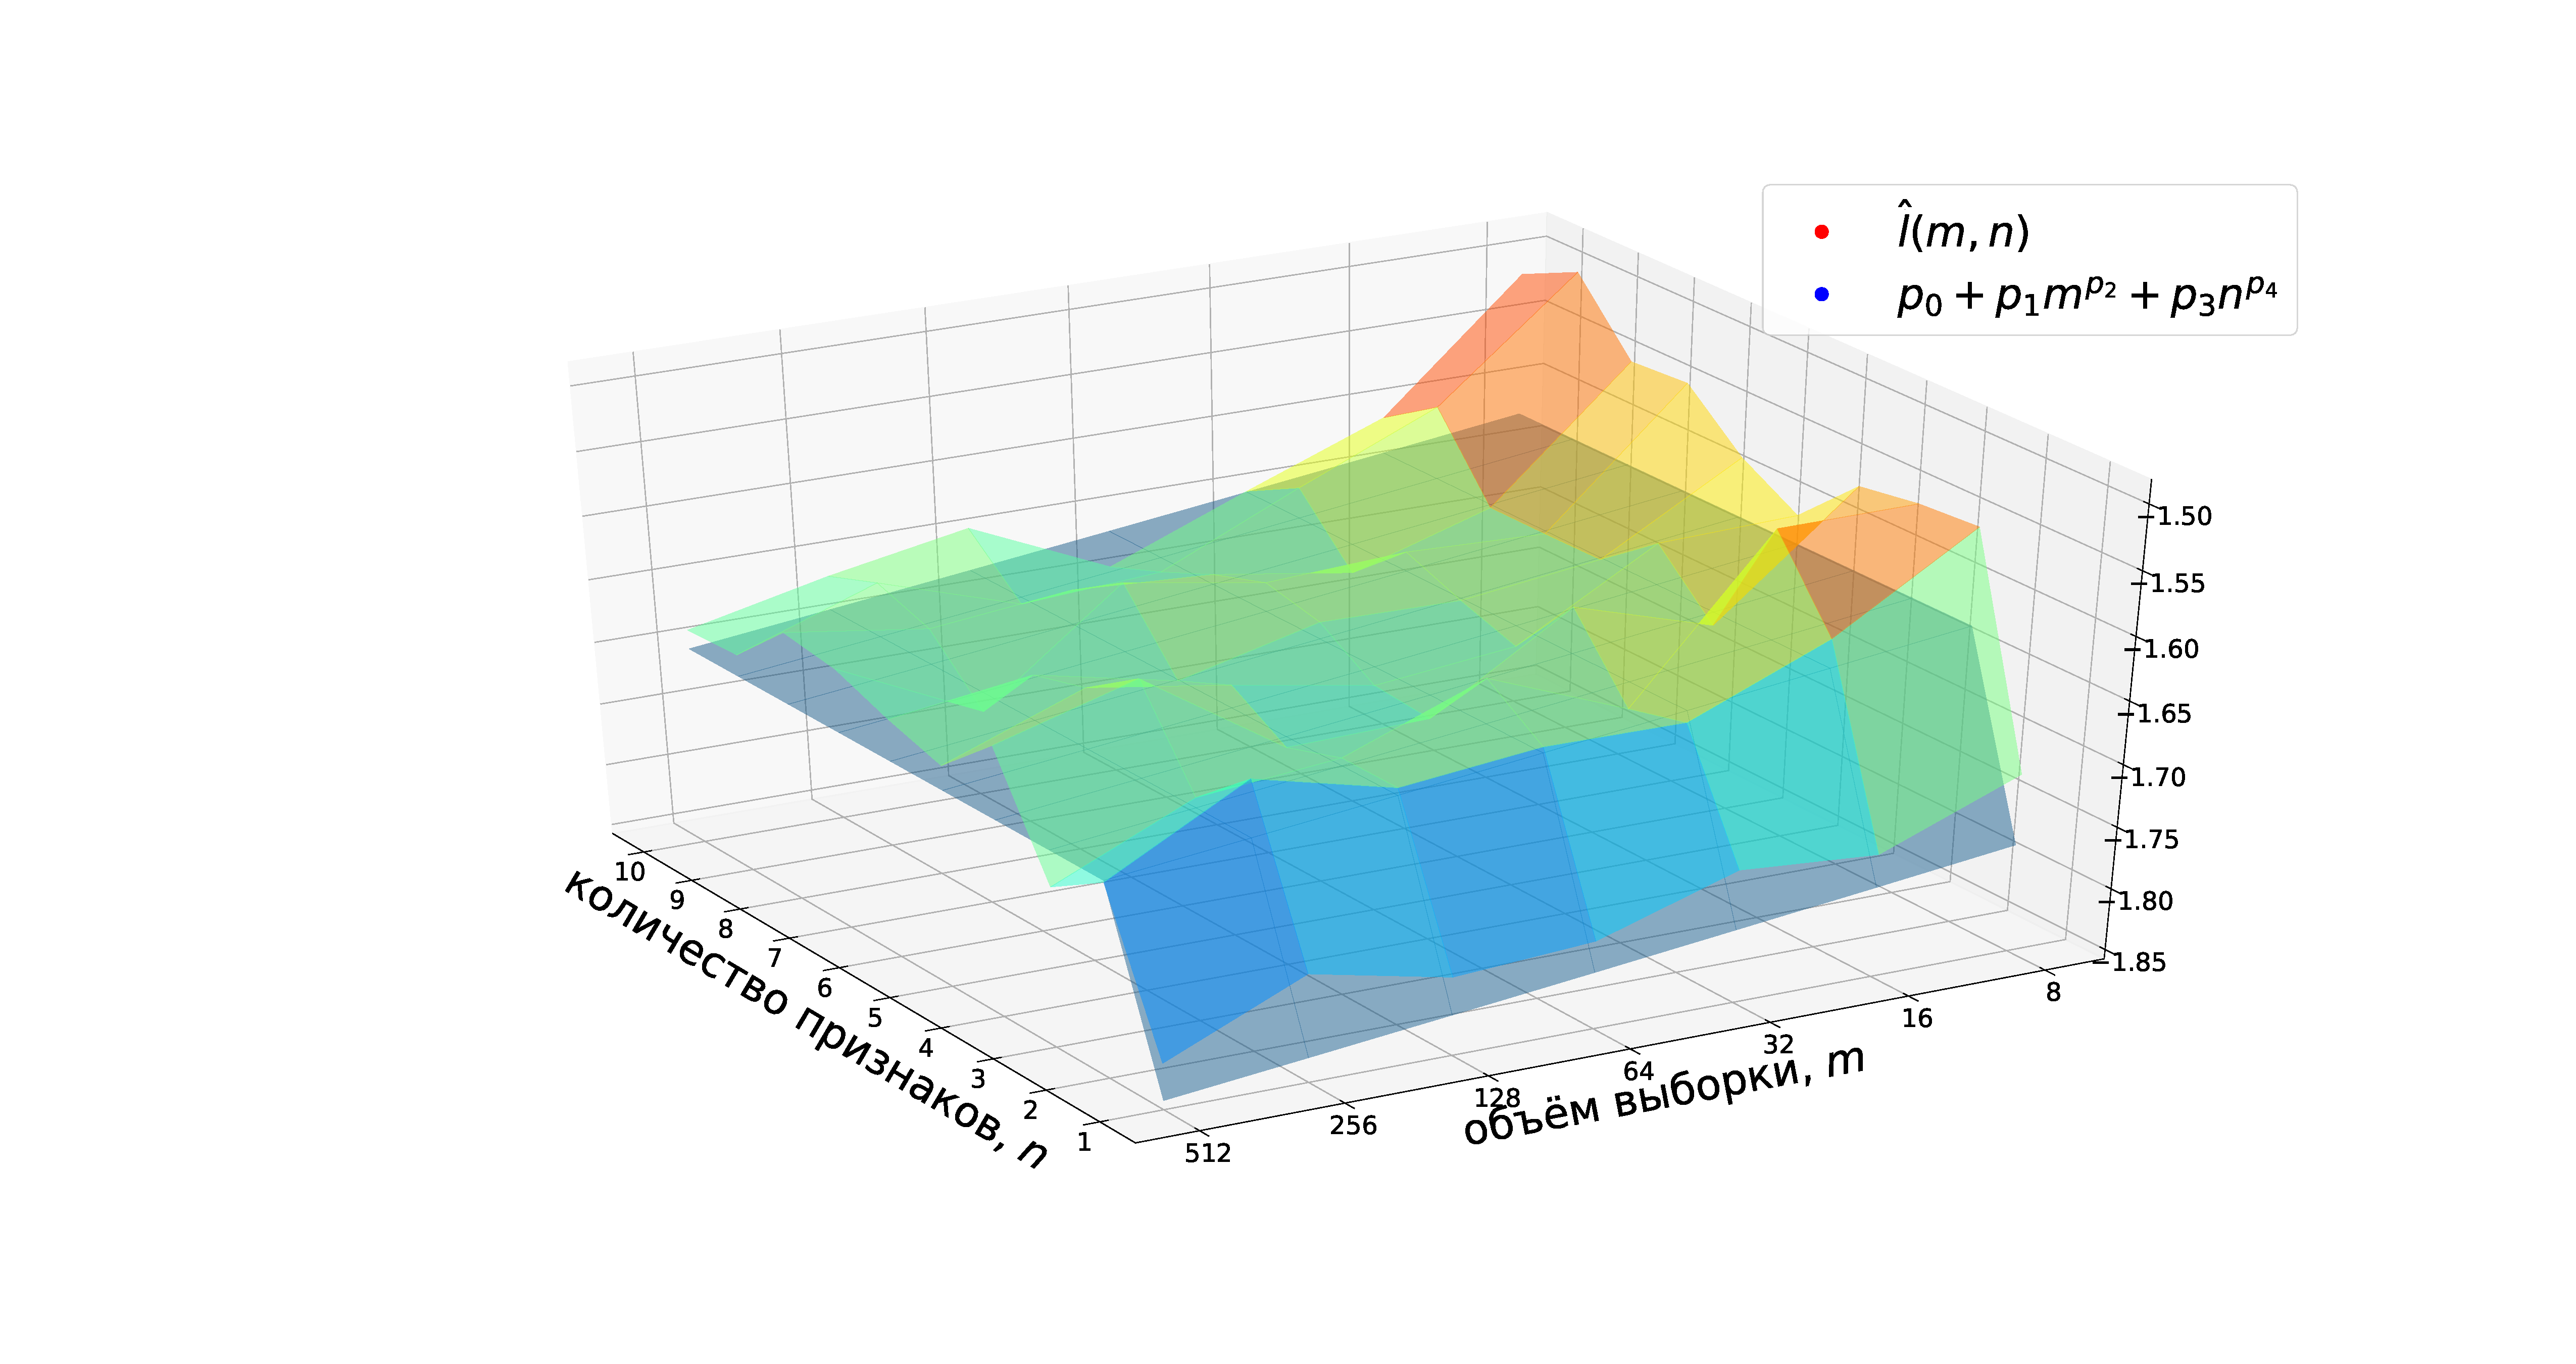
\includegraphics[width=0.5\textwidth]{../data/pics/exploitational_adequate_correlated_sample_llh_phi.pdf}}\\
\subfloat[Адекватная ортогональная выборка]{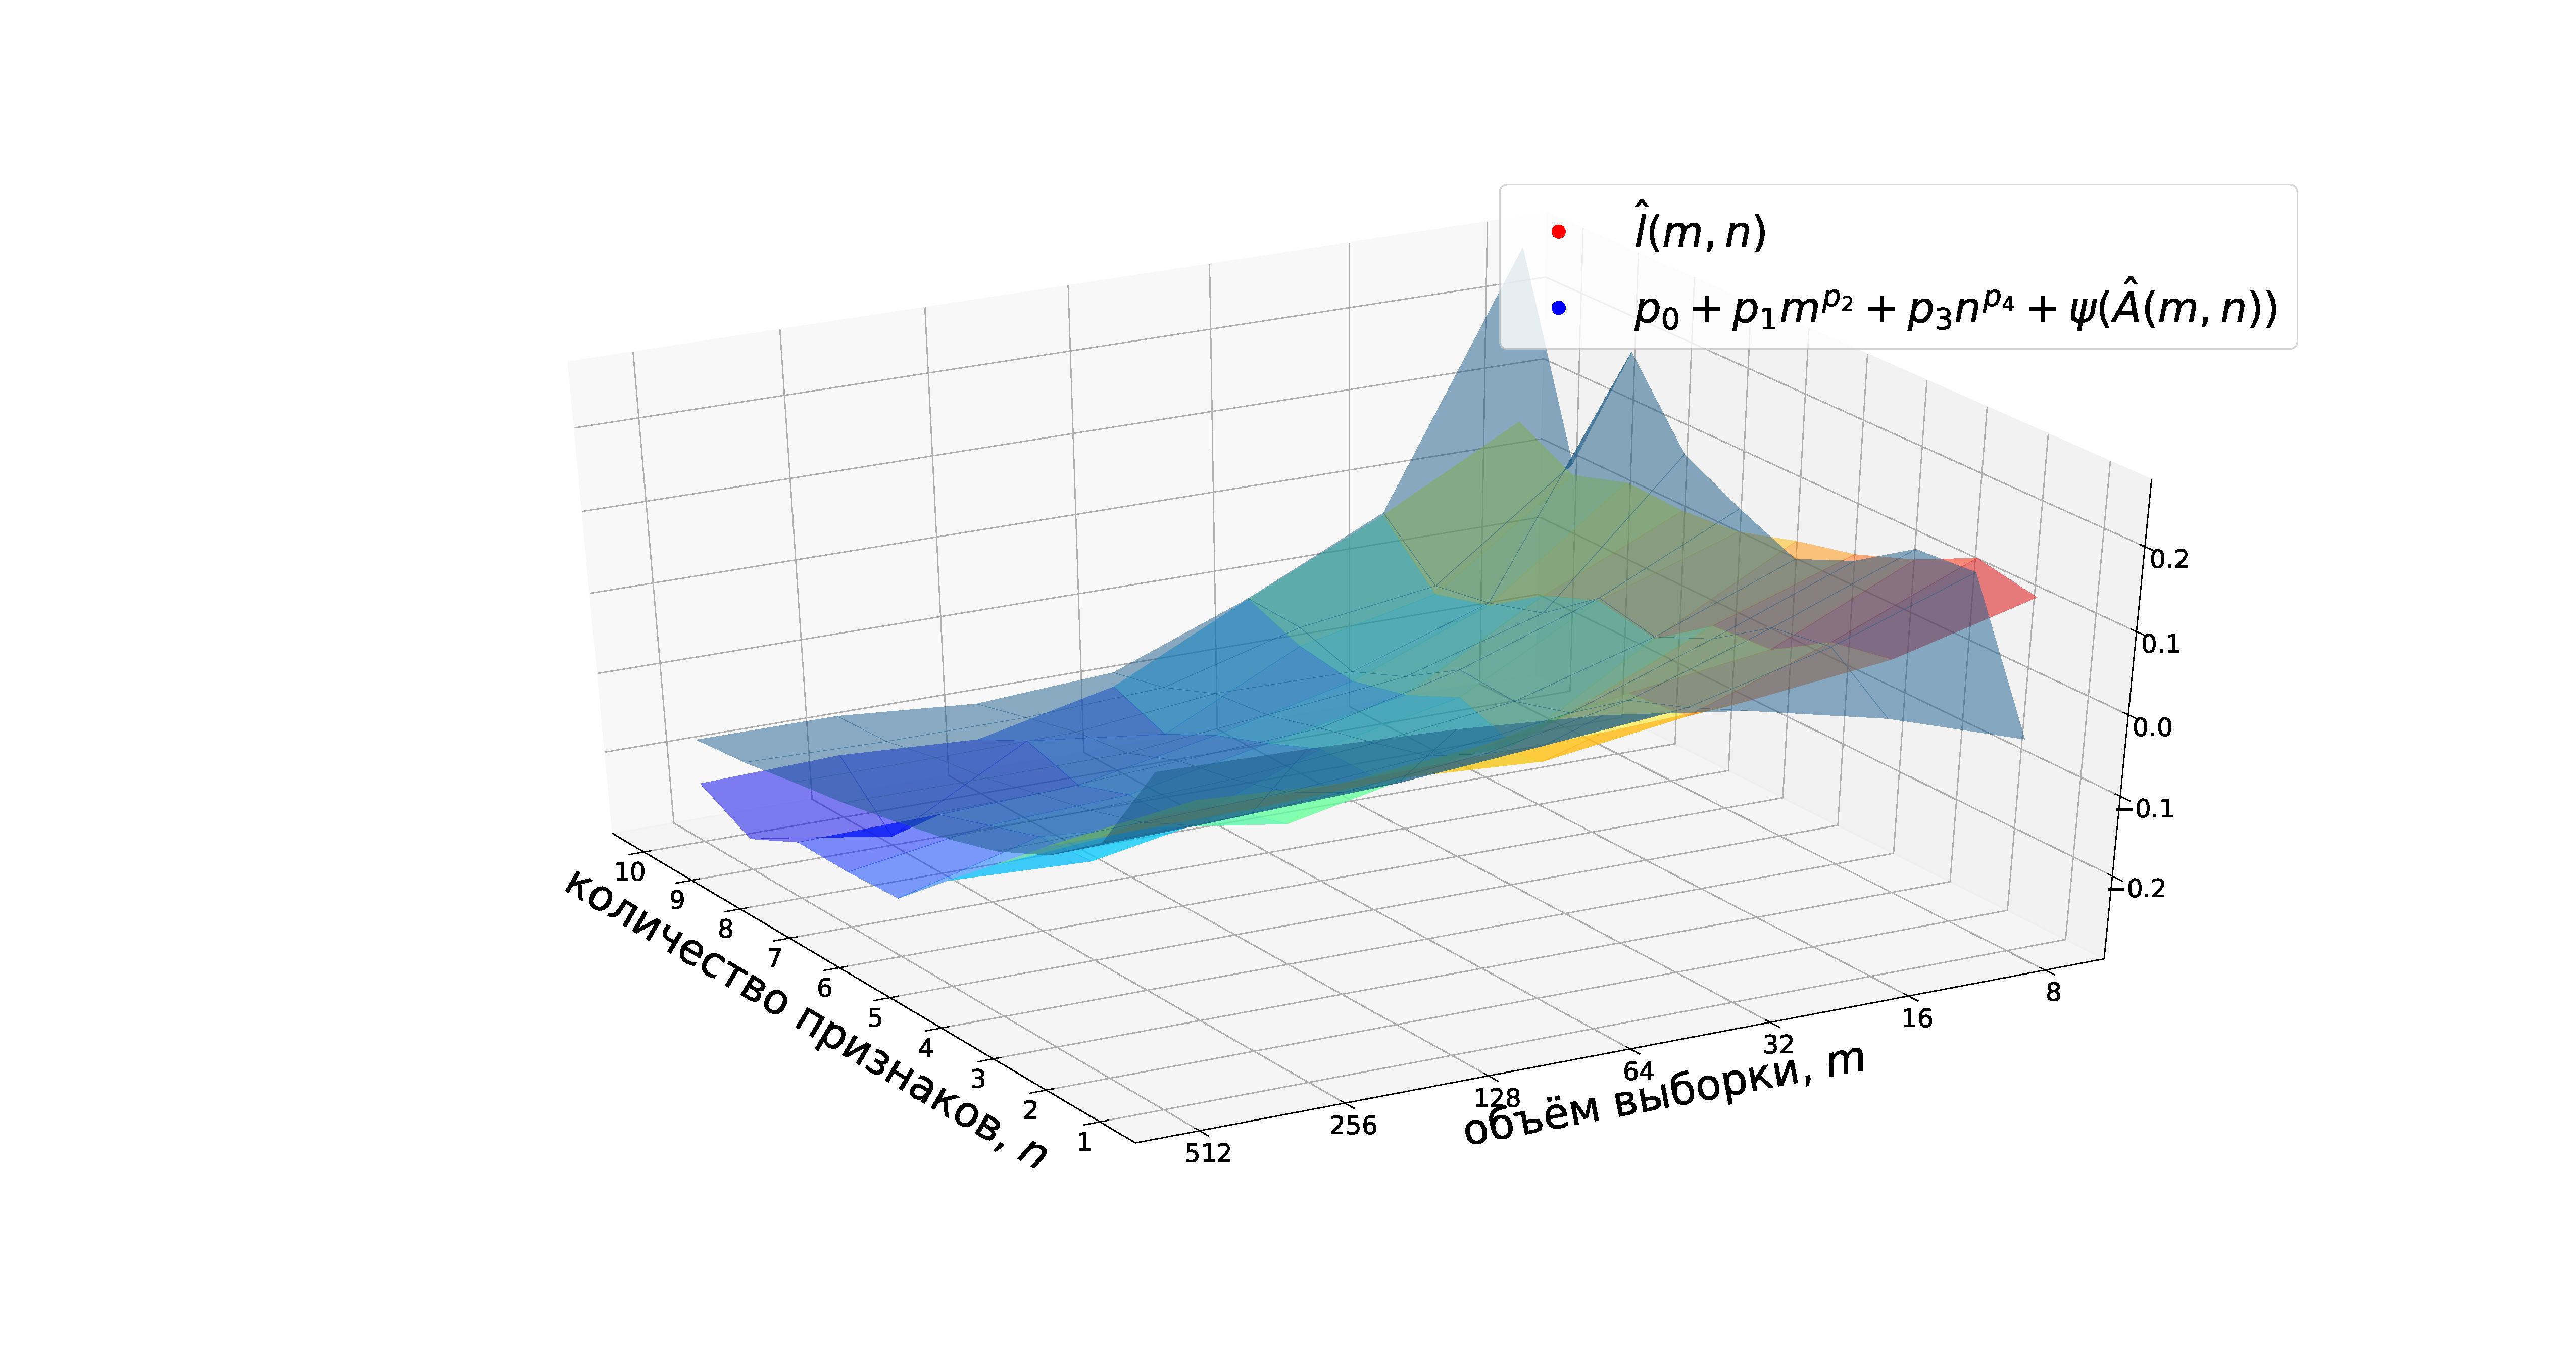
\includegraphics[width=0.5\textwidth]{../data/pics/theoretical_adequate_orthogonal_sample_llh_phi.pdf}}&
\subfloat[Адекватная ортогональная выборка]{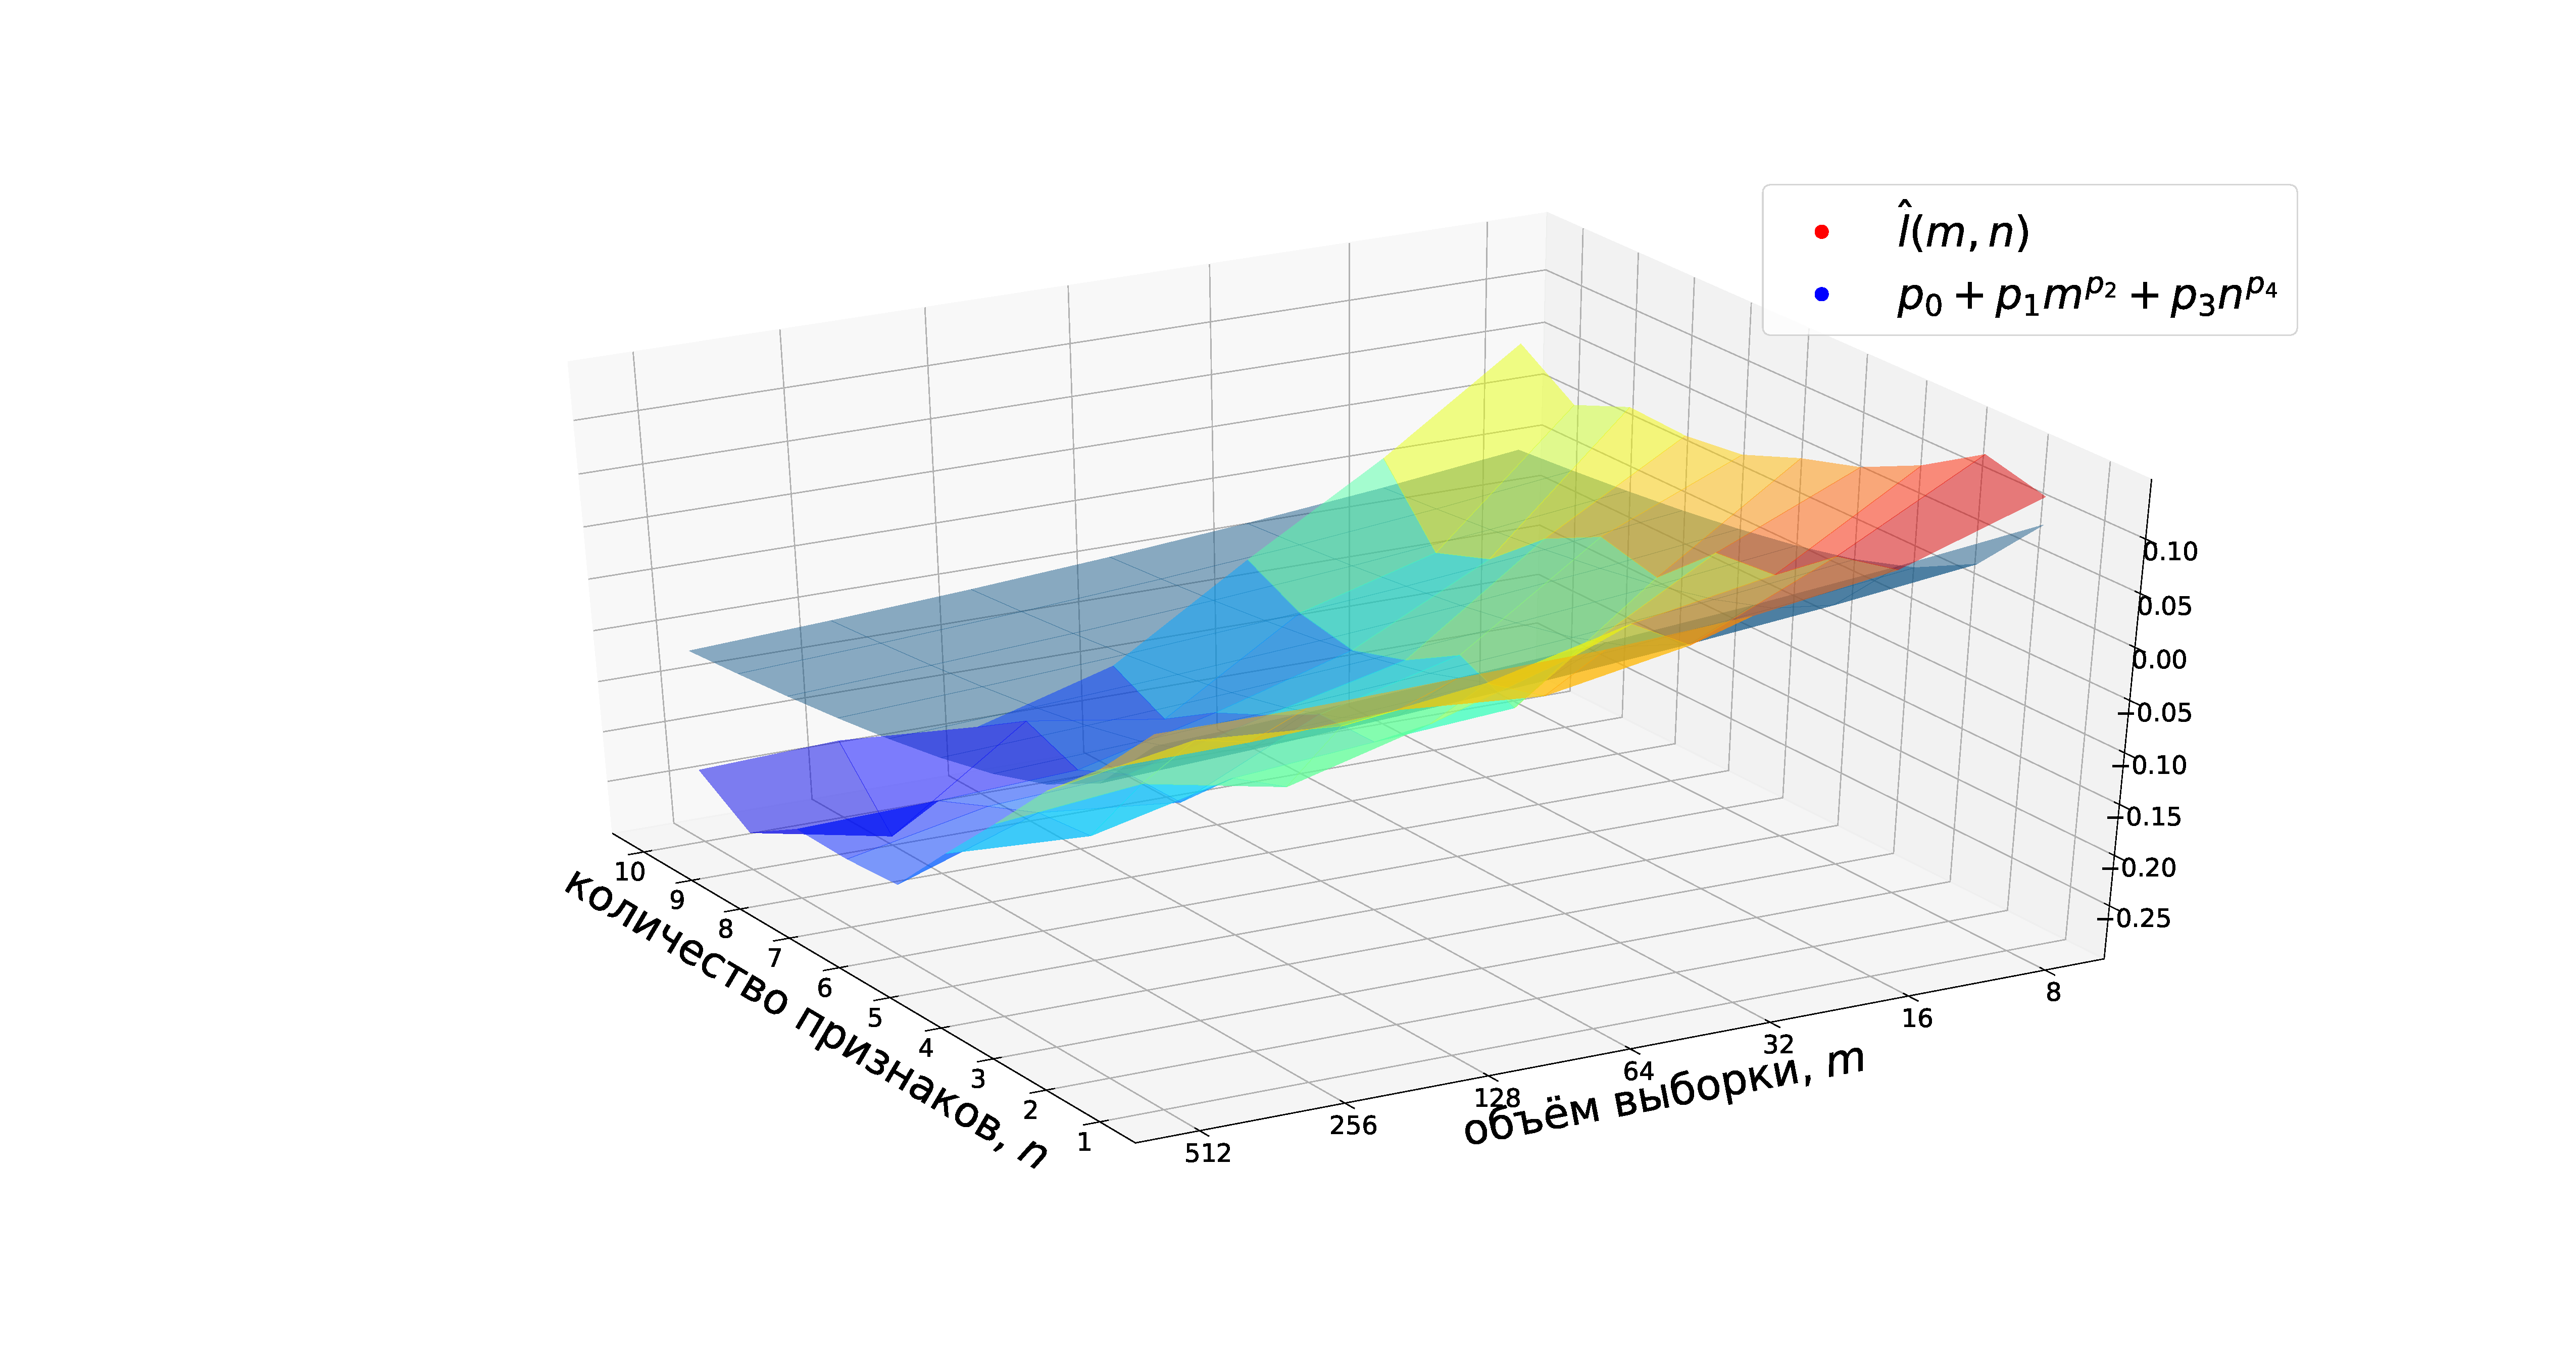
\includegraphics[width=0.5\textwidth]{../data/pics/exploitational_adequate_orthogonal_sample_llh_phi.pdf}}\\
\subfloat[Адекватная избыточная выборка]{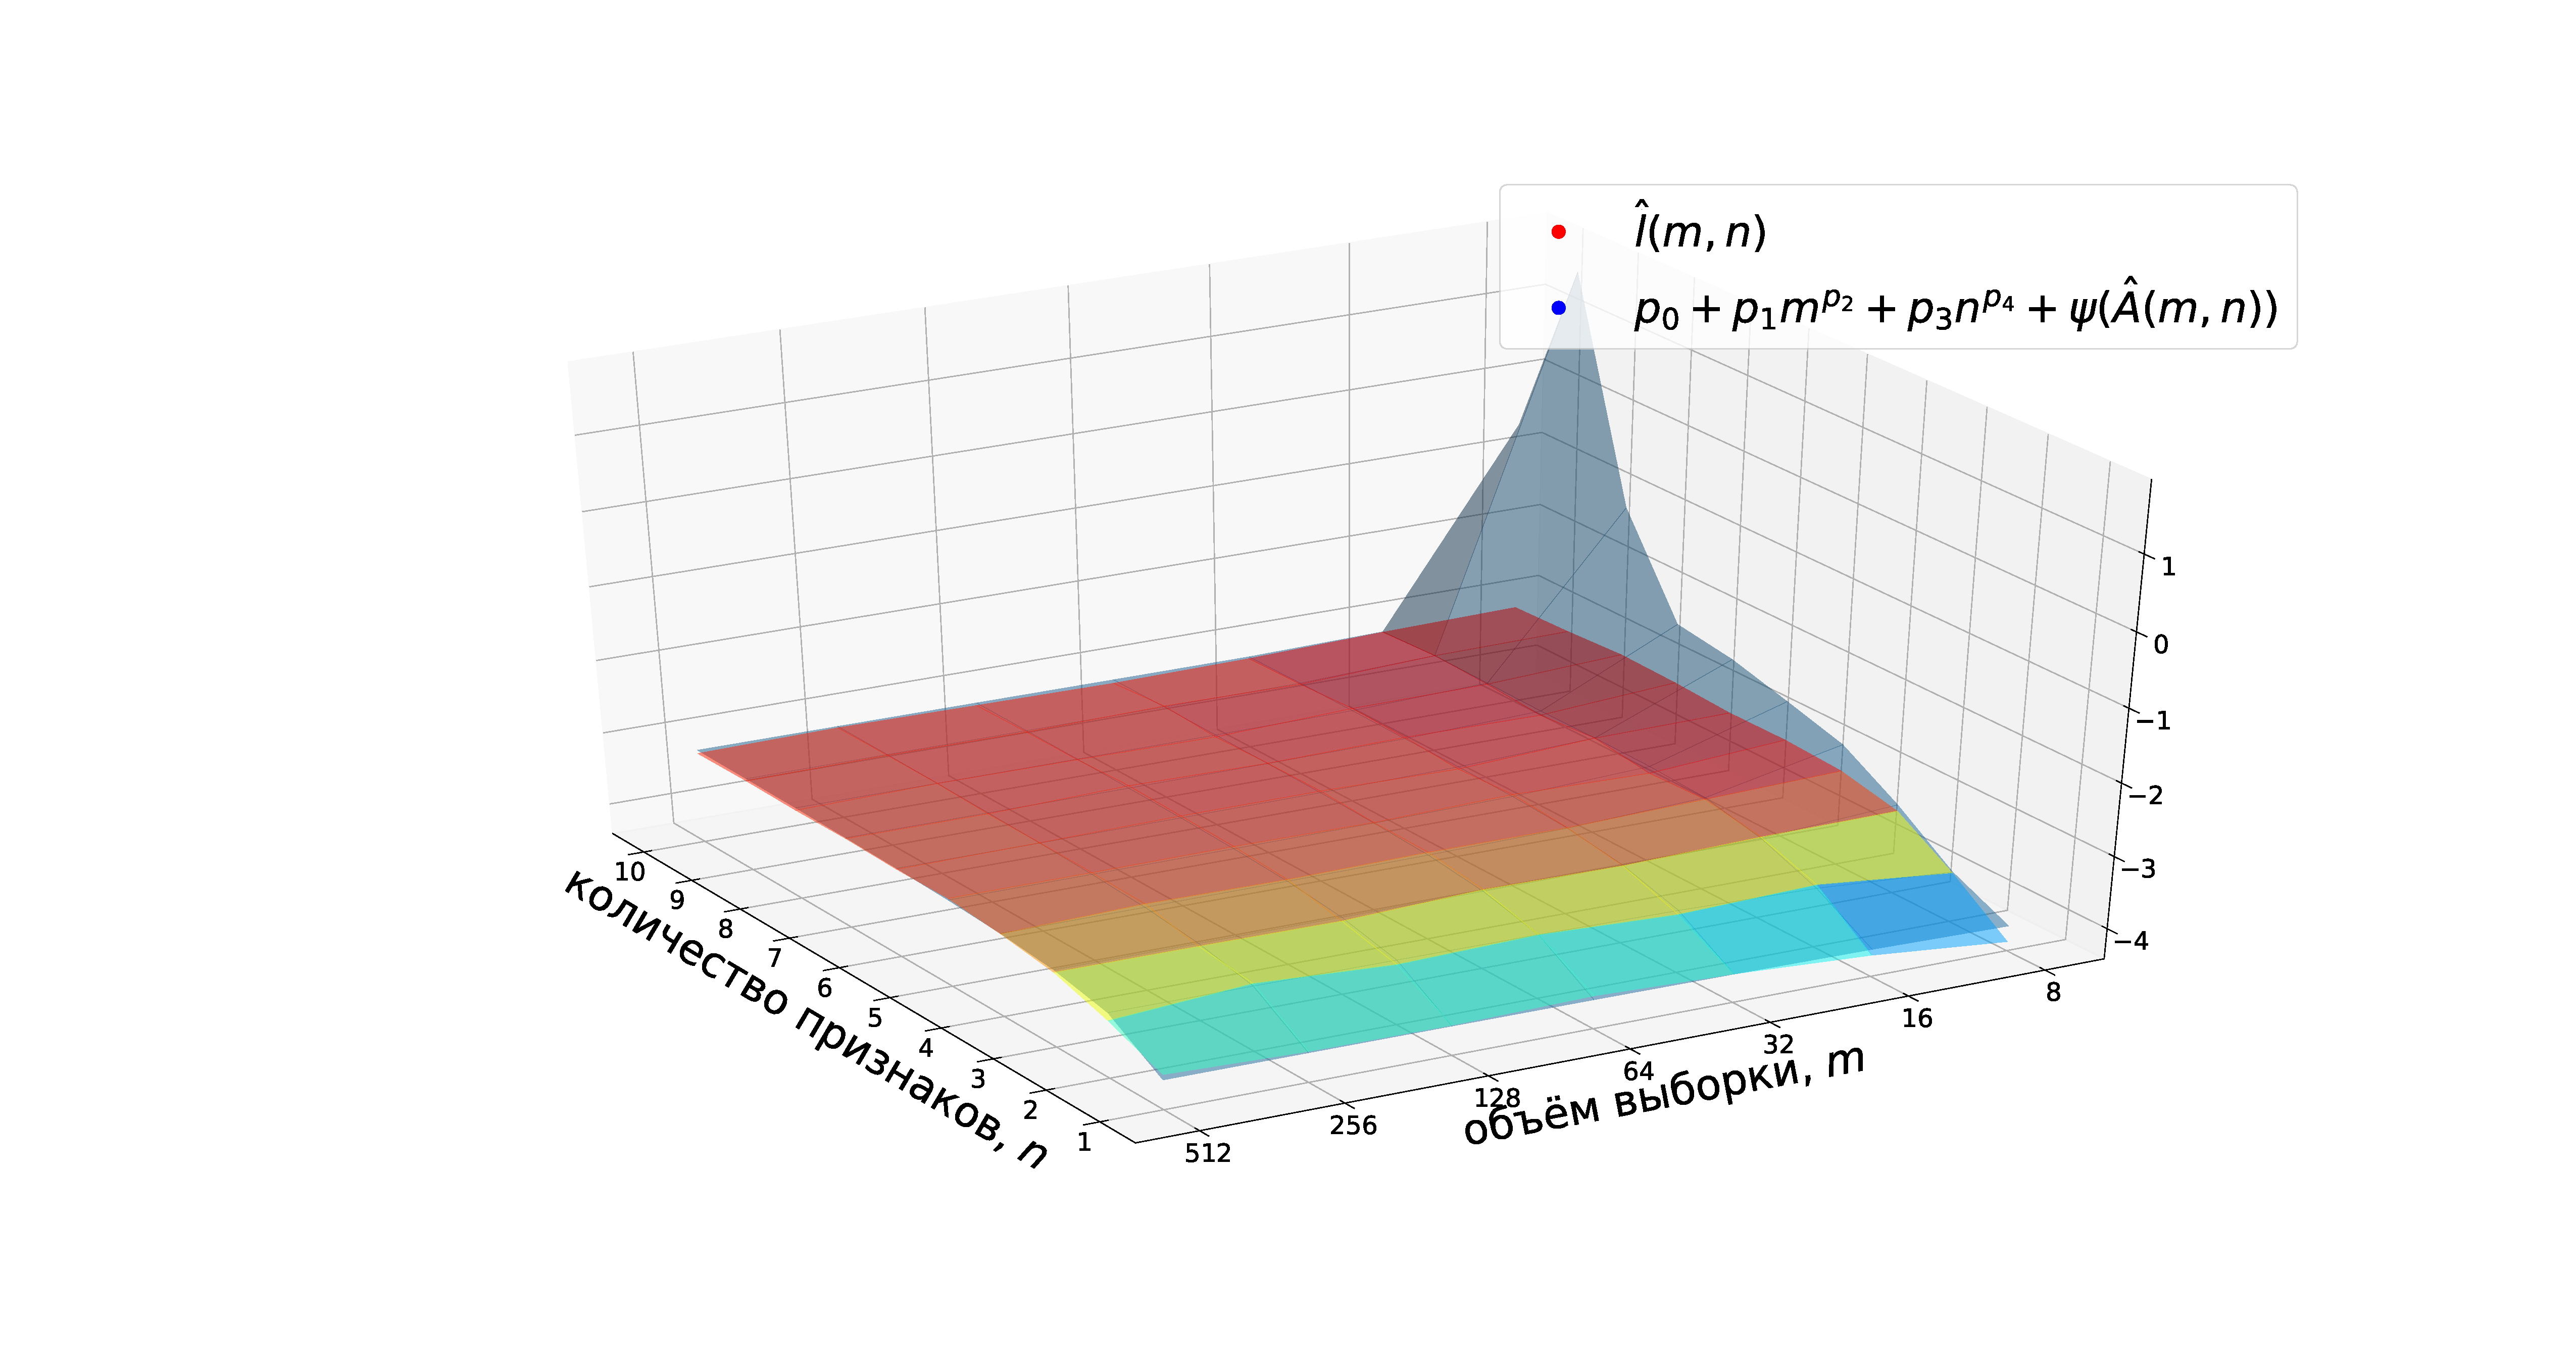
\includegraphics[width=0.5\textwidth]{../data/pics/theoretical_adequate_redundant_sample_llh_phi.pdf}}&
\subfloat[Адекватная избыточная выборка]{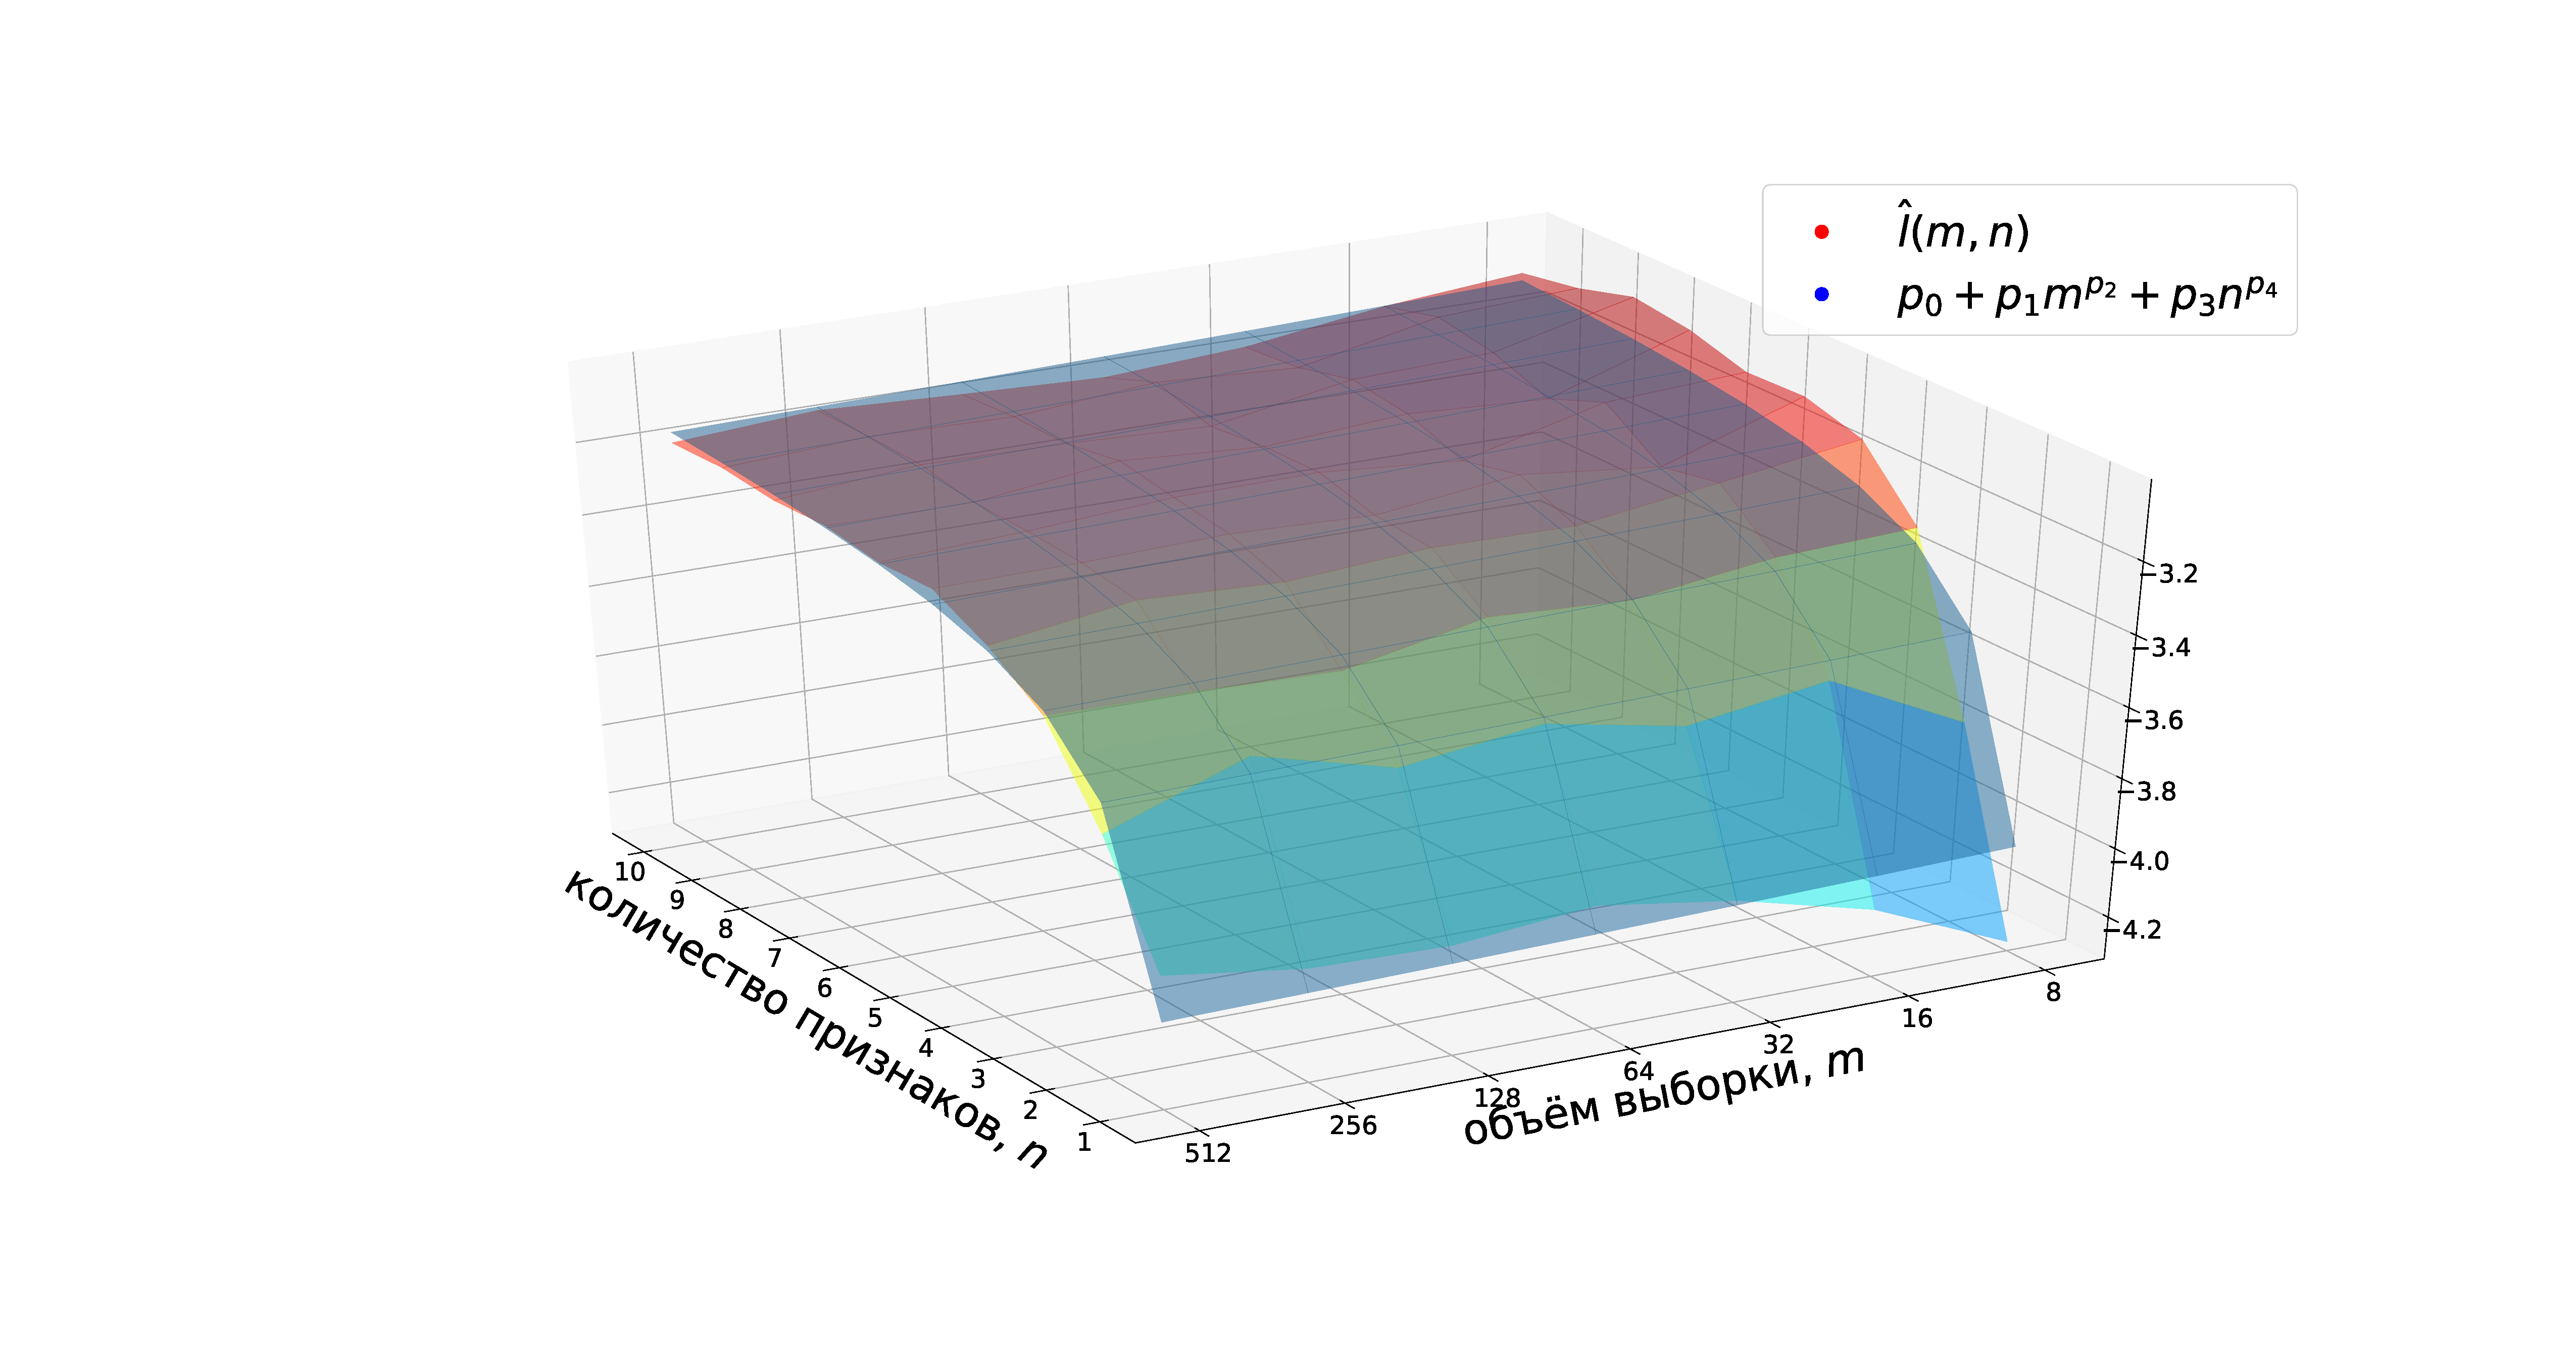
\includegraphics[width=0.5\textwidth]{../data/pics/exploitational_adequate_redundant_sample_llh_phi.pdf}}\\
\end{tabular}

\caption{Зависимость значения функции $\hat{l}(m, n)$ от объема выборки $m$ и количества параметров $n$}
\label{fig101}
\end{figure}

На рис. 4 представлены функции ошибки MAPE для 4 функций $\phi \in \Phi$, аппроксимирующих $\hat{l}$, посчитанную в теоретическом и эмпирическом вариантах, с использованием или без использования ковариационной матрицы $\hat{A}$ вектора параметров $\hat{\mathbf{w}}$.

\begin{figure}[h!t]\center
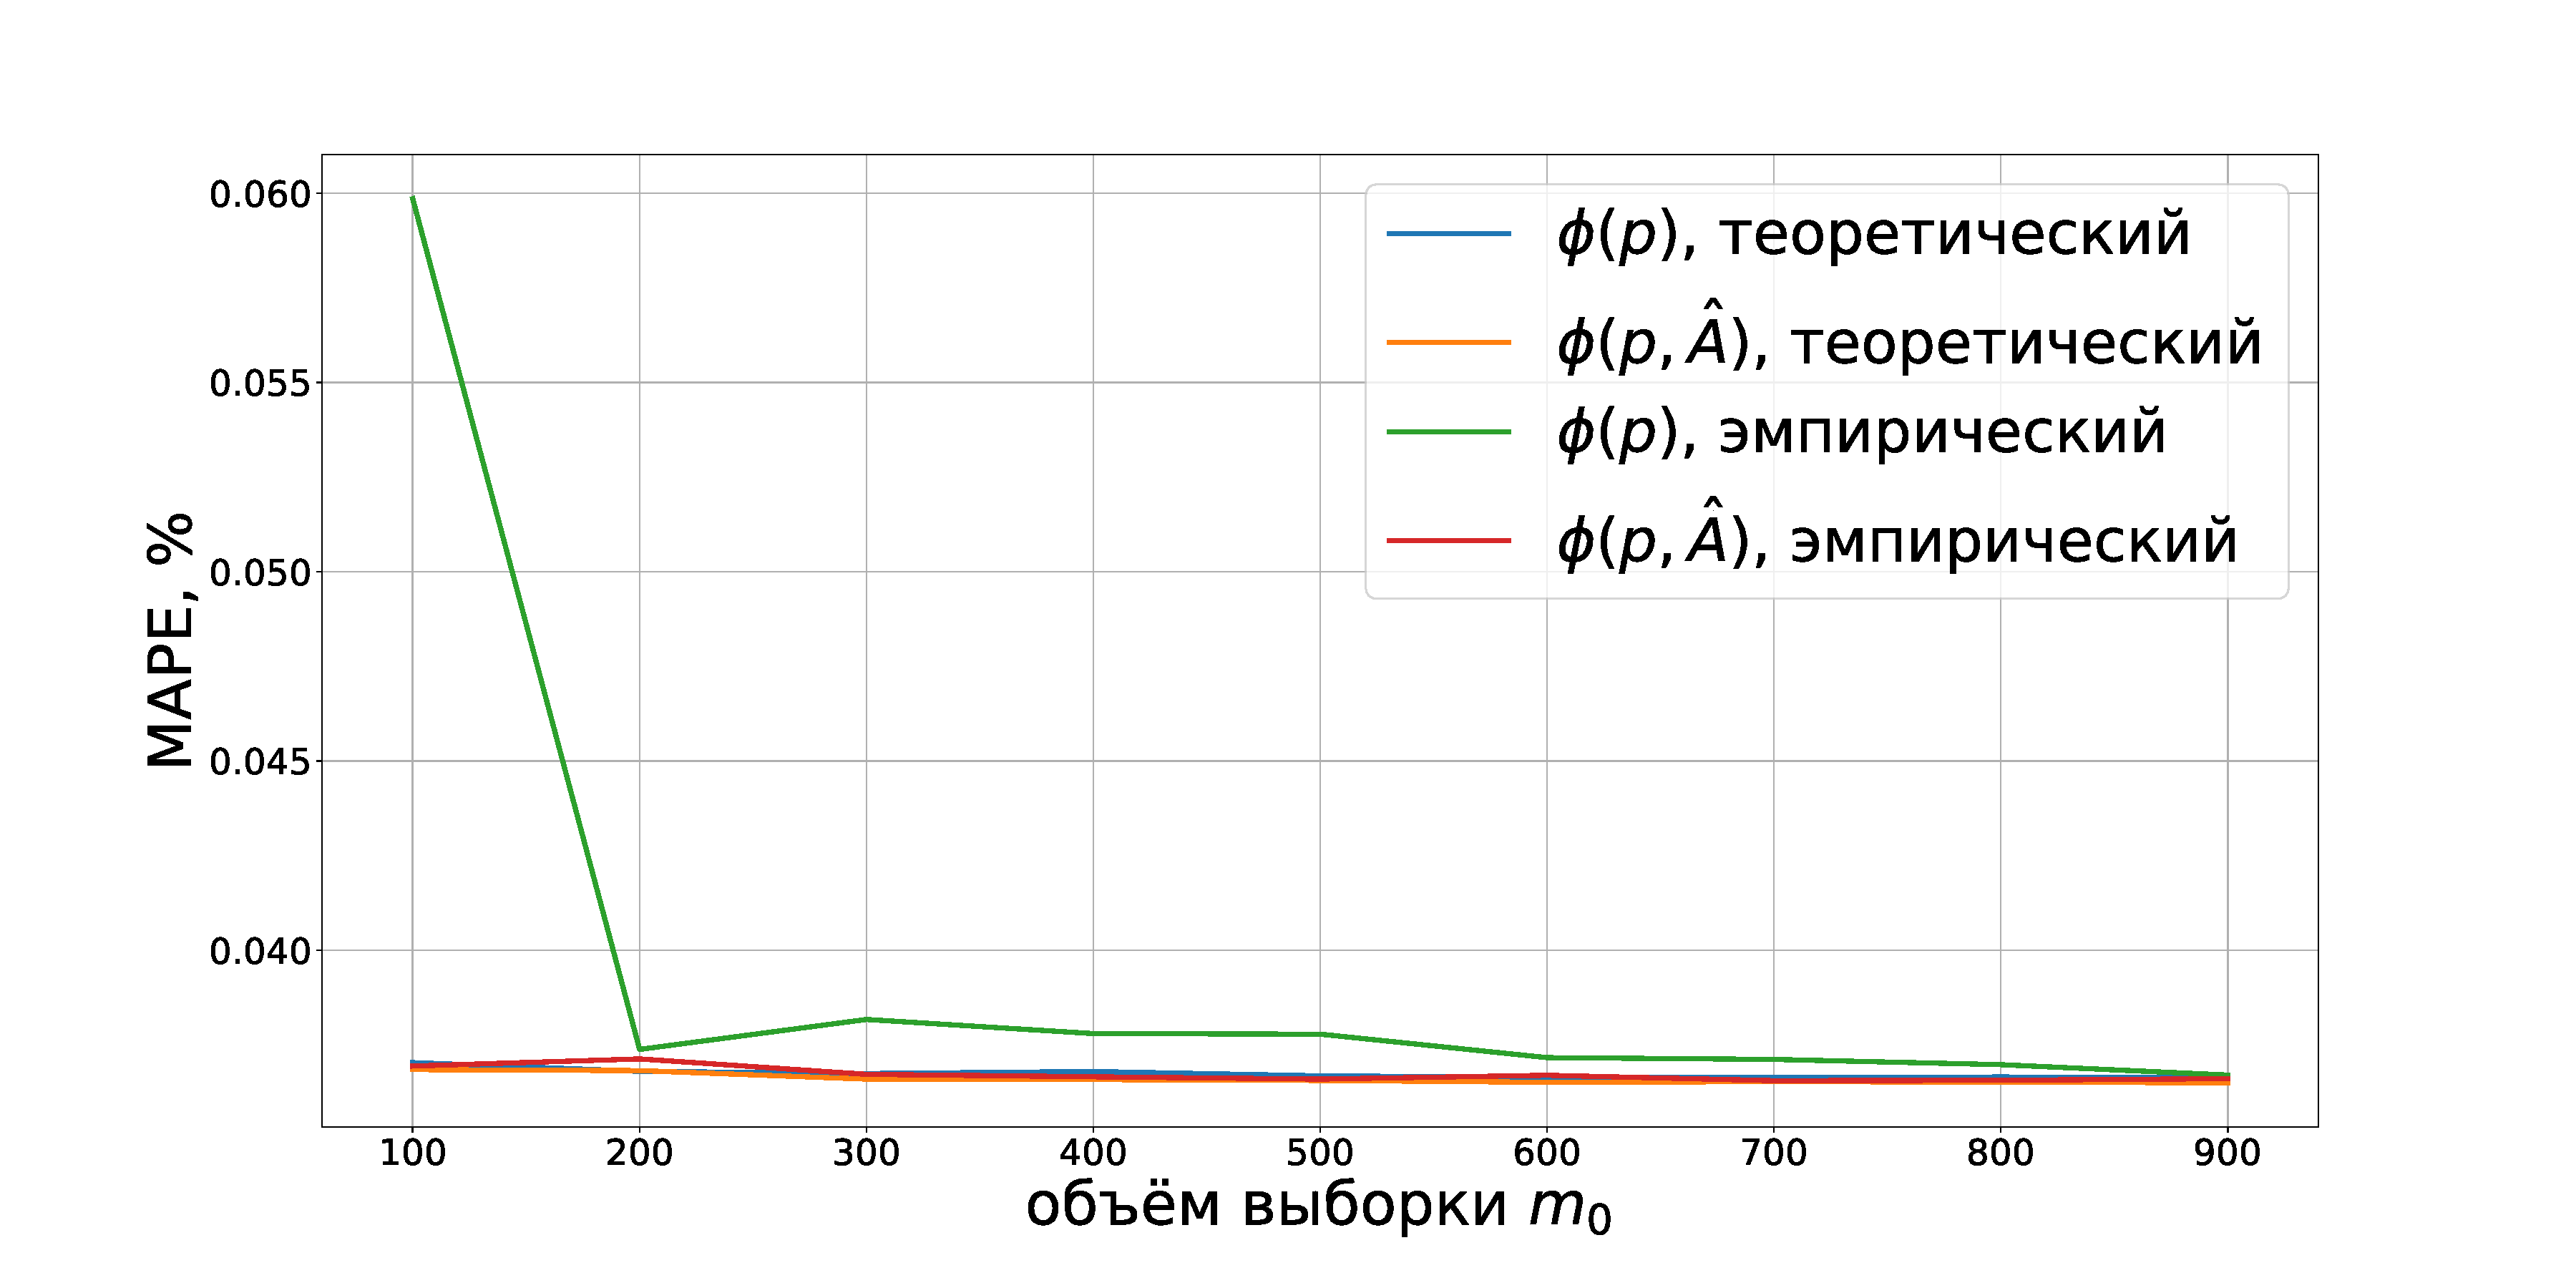
\includegraphics[width=1\textwidth]{../data/pics/adequate_random_sample_MAPE_comparison.pdf}
\caption{Функции $\hat{l}(m, n)$ и $\phi(p, \hat{A}(m, n), m, n)$ для адекватной случайной выборки}
\label{fig1.7}
\end{figure}

\subsection{Использование оценки $\hat{A}$ для вычисления объёма $m_0$}

На рис. 5 представлена зависимость элементов ковариационной матрицы вектора параметров от объема выборки. [Комментарий?].
Зависимость посчитана с помощью метода бутстреп:
\begin{enumerate}
	\item Генерируется случайная подвыборка $\mathfrak D_{\mathcal{L}} \subset \mathfrak D$, $|\mathfrak D_{\mathcal{L}}| = m$
	\item Вычисляется оценка вектора параметров $\hat{\mathbf{w}}_k$ как решение оптимизационной задачи (\ref{argmax_L}) на выборке $\mathfrak D_{\mathcal{L}}$.
	\item Вычисляется оценка ковариационной матрицы параметров $\hat{A}_k$ по формуле:
\begin{equation}\label{Ahat}
\hat{A}_k =  \frac{1}{n}(\hat{\mathbf{w}}_k - \overline{\hat{\mathbf{w}}})^{\top}(\hat{\mathbf{w}}_k - \overline{\hat{\mathbf{w}}}).
\end{equation}
	\item пп. 1-3 повторяются $K$ раз, итоговая оценка равна среднему значению среди полученных оценок матрицы ковариации (\ref{Ahat}).
\end{enumerate}

На рис. 6 представлена зависимость элементов матрицы Фишера от объема выборки. Оценка информационной матрицы Фишера $\hat{I}$ выражена через оценку ковариационной матрицы по формуле (\ref{w_hat_I}).

$\newline$
$\newline$
$\newline$
$\newline$
$\newline$
$\newline$
$\newline$
$\newline$
$\newline$
$\newline$
$\newline$
$\newline$
$\newline$
$\newline$

\begin{figure}[h!t]\center
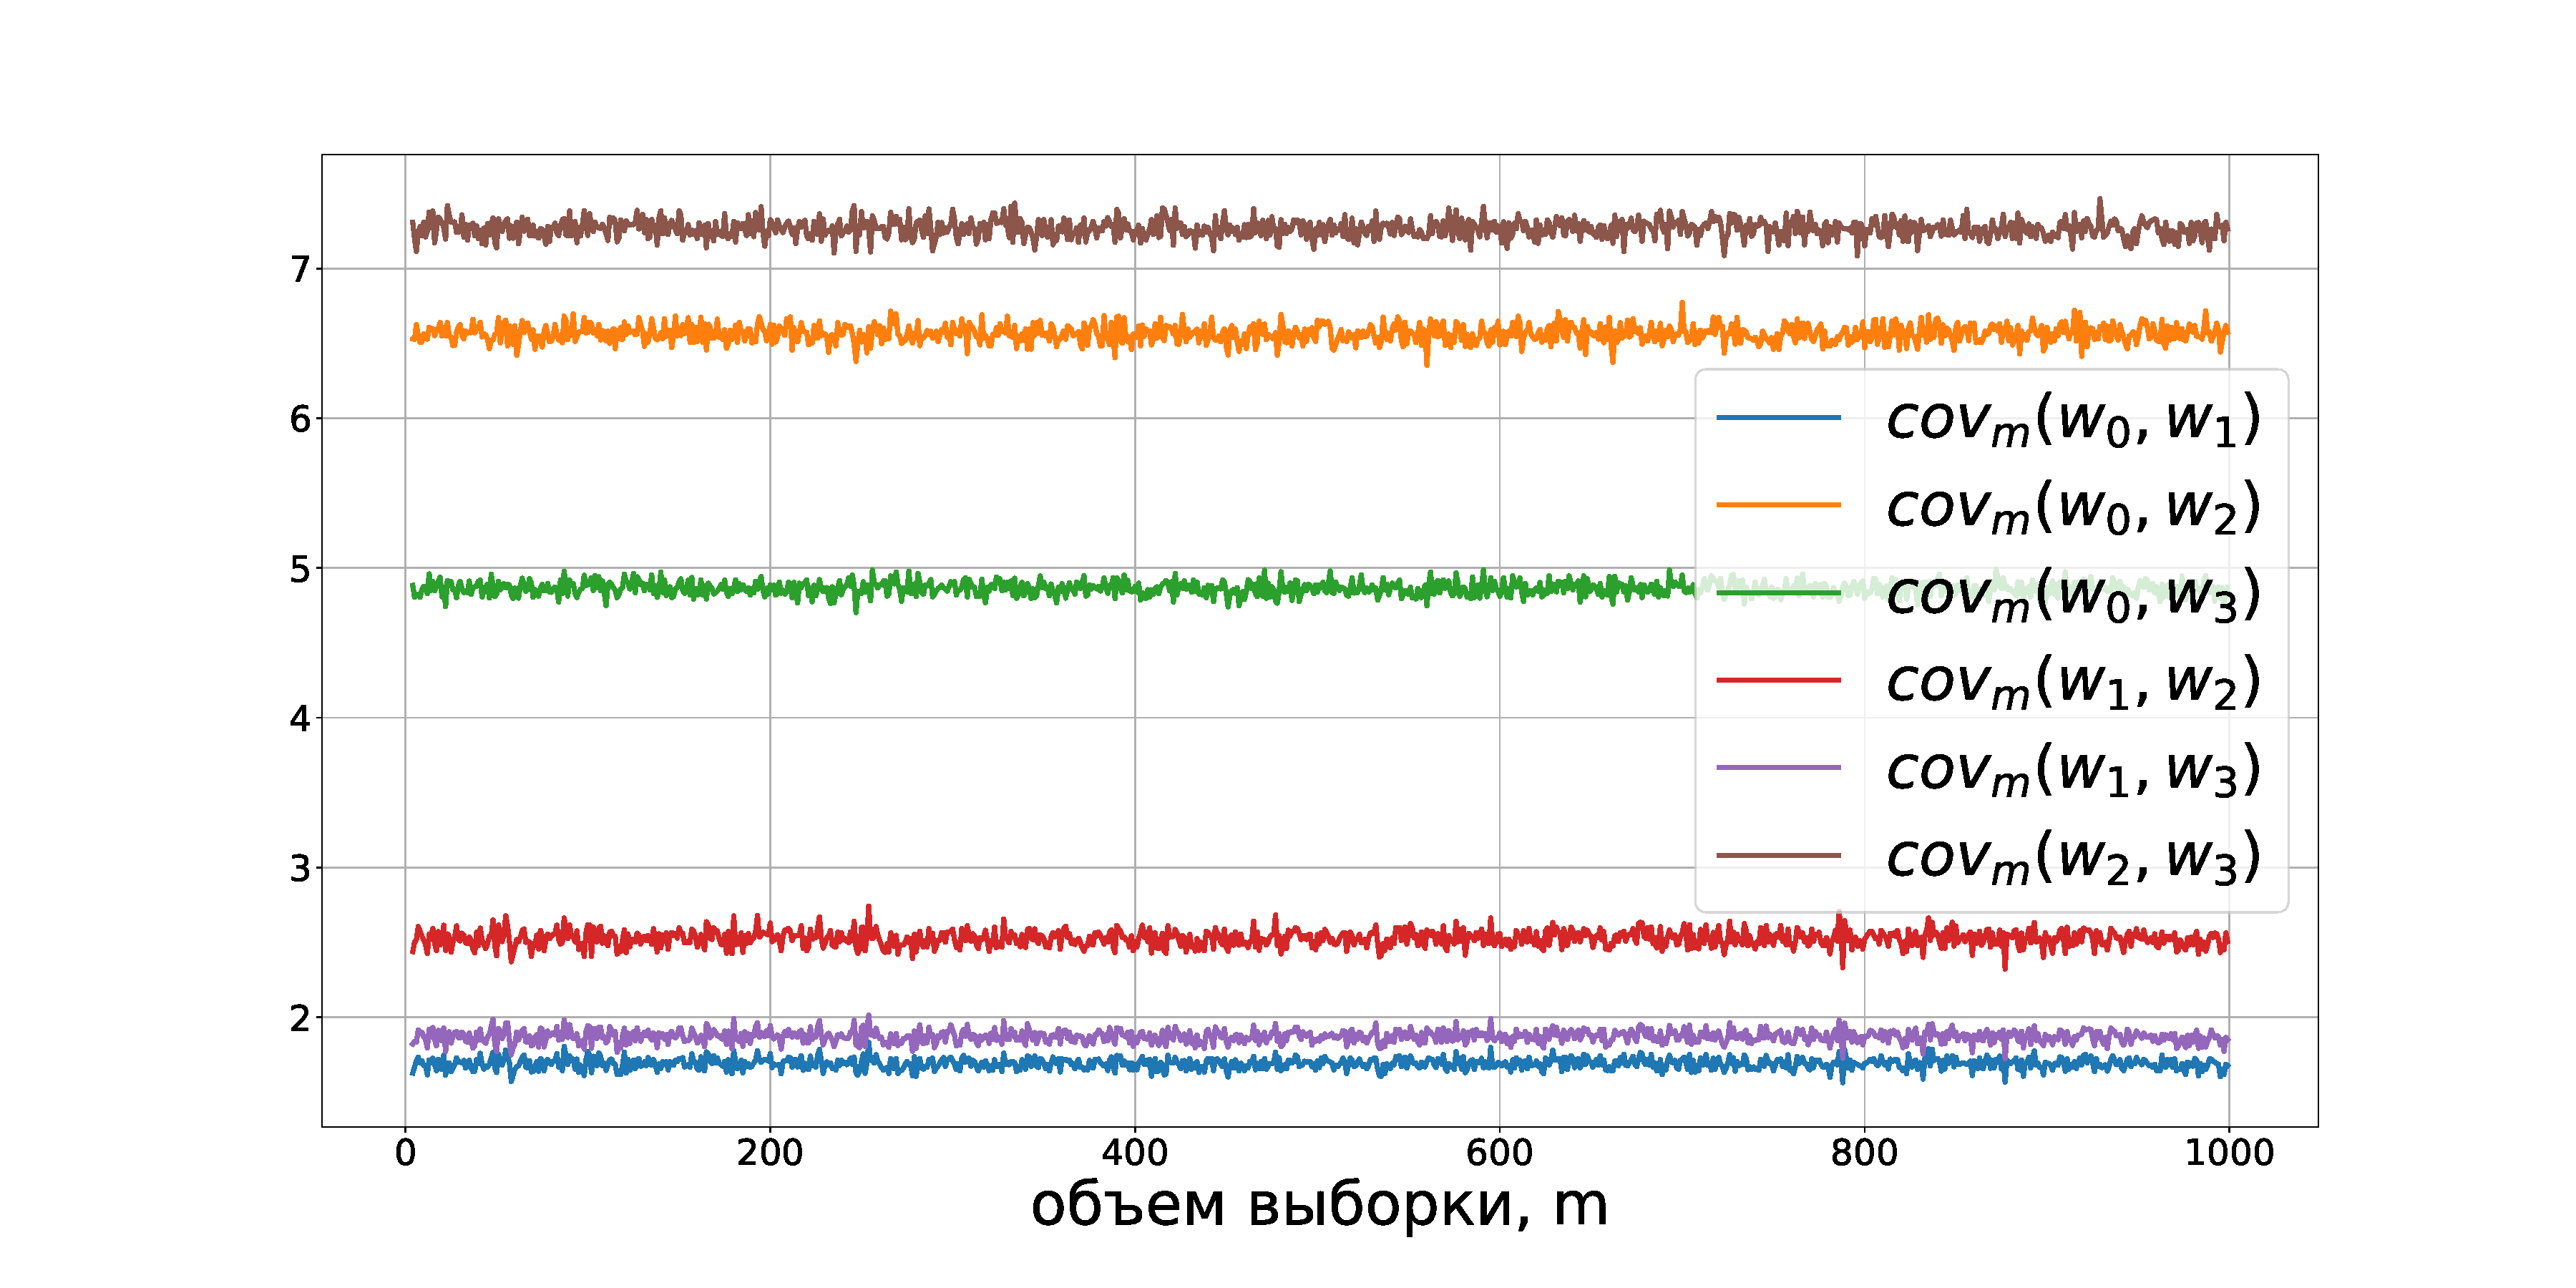
\includegraphics[width=1\textwidth]{../data/pics/synthetic_W.pdf}
\caption{Зависимость значения элементов ковариационной матрицы от объема выборки}
\label{fig2}
\end{figure}

\begin{figure}[h!t]\center
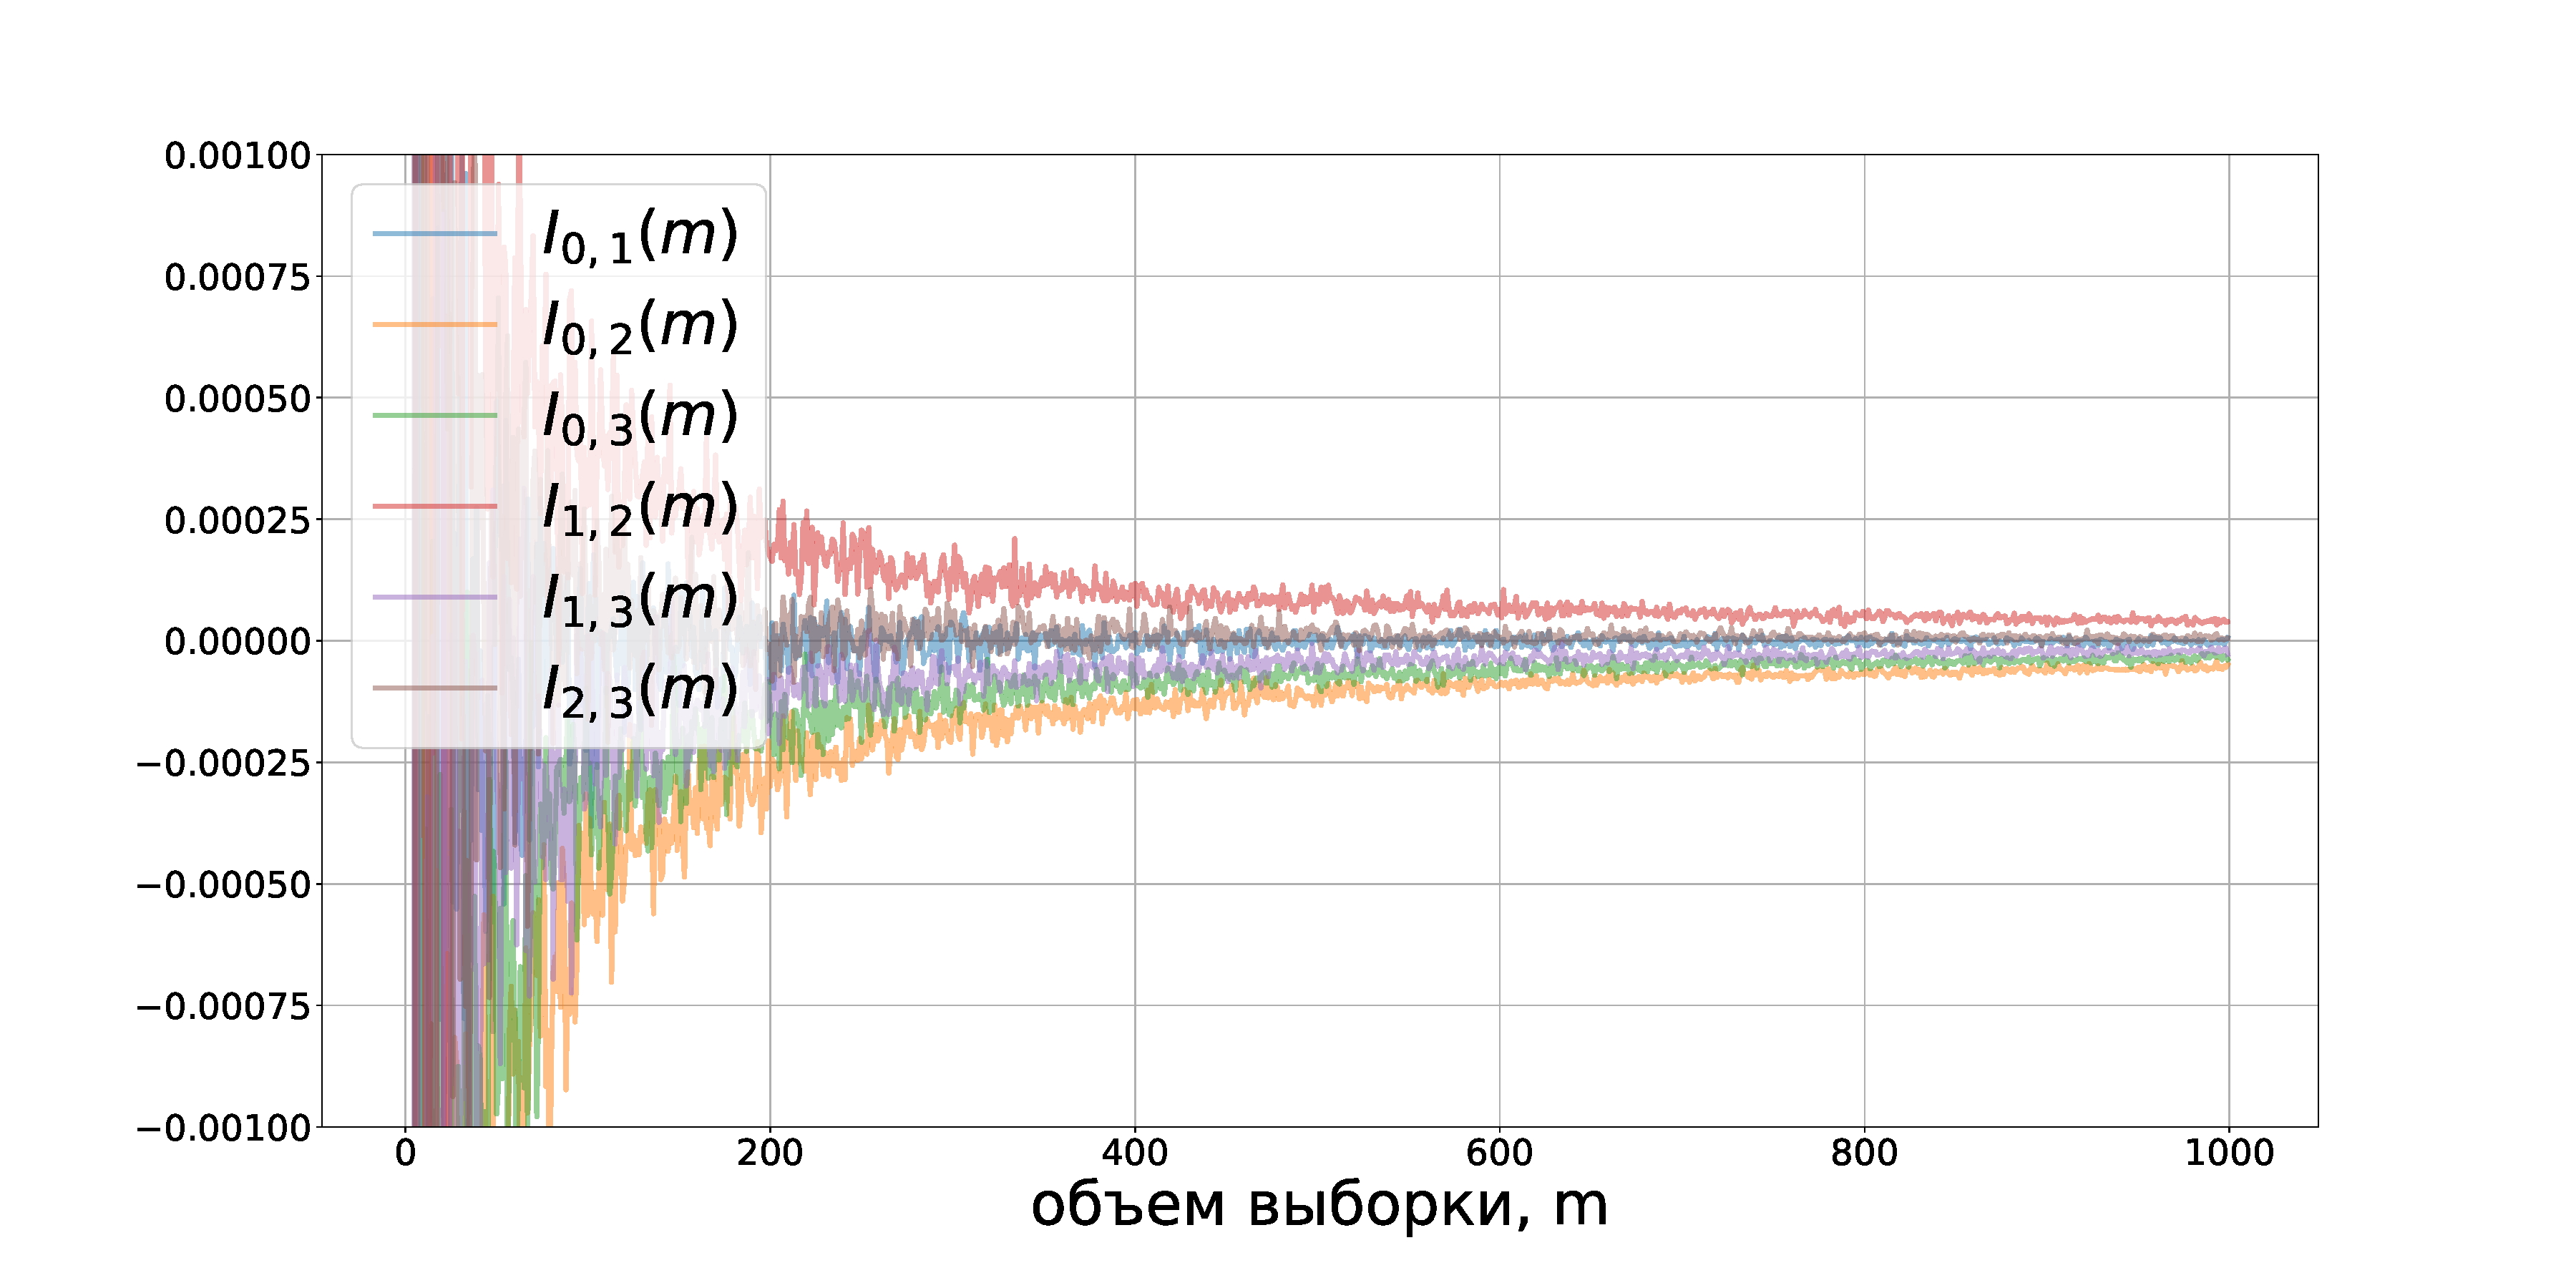
\includegraphics[width=1\textwidth]{../data/pics/synthetic_I.pdf}
\caption{Зависимость значения элементов матрицы Фишера от объема выборки}
\label{fig3}
\end{figure}

%\begin{figure}[h!t]\center
%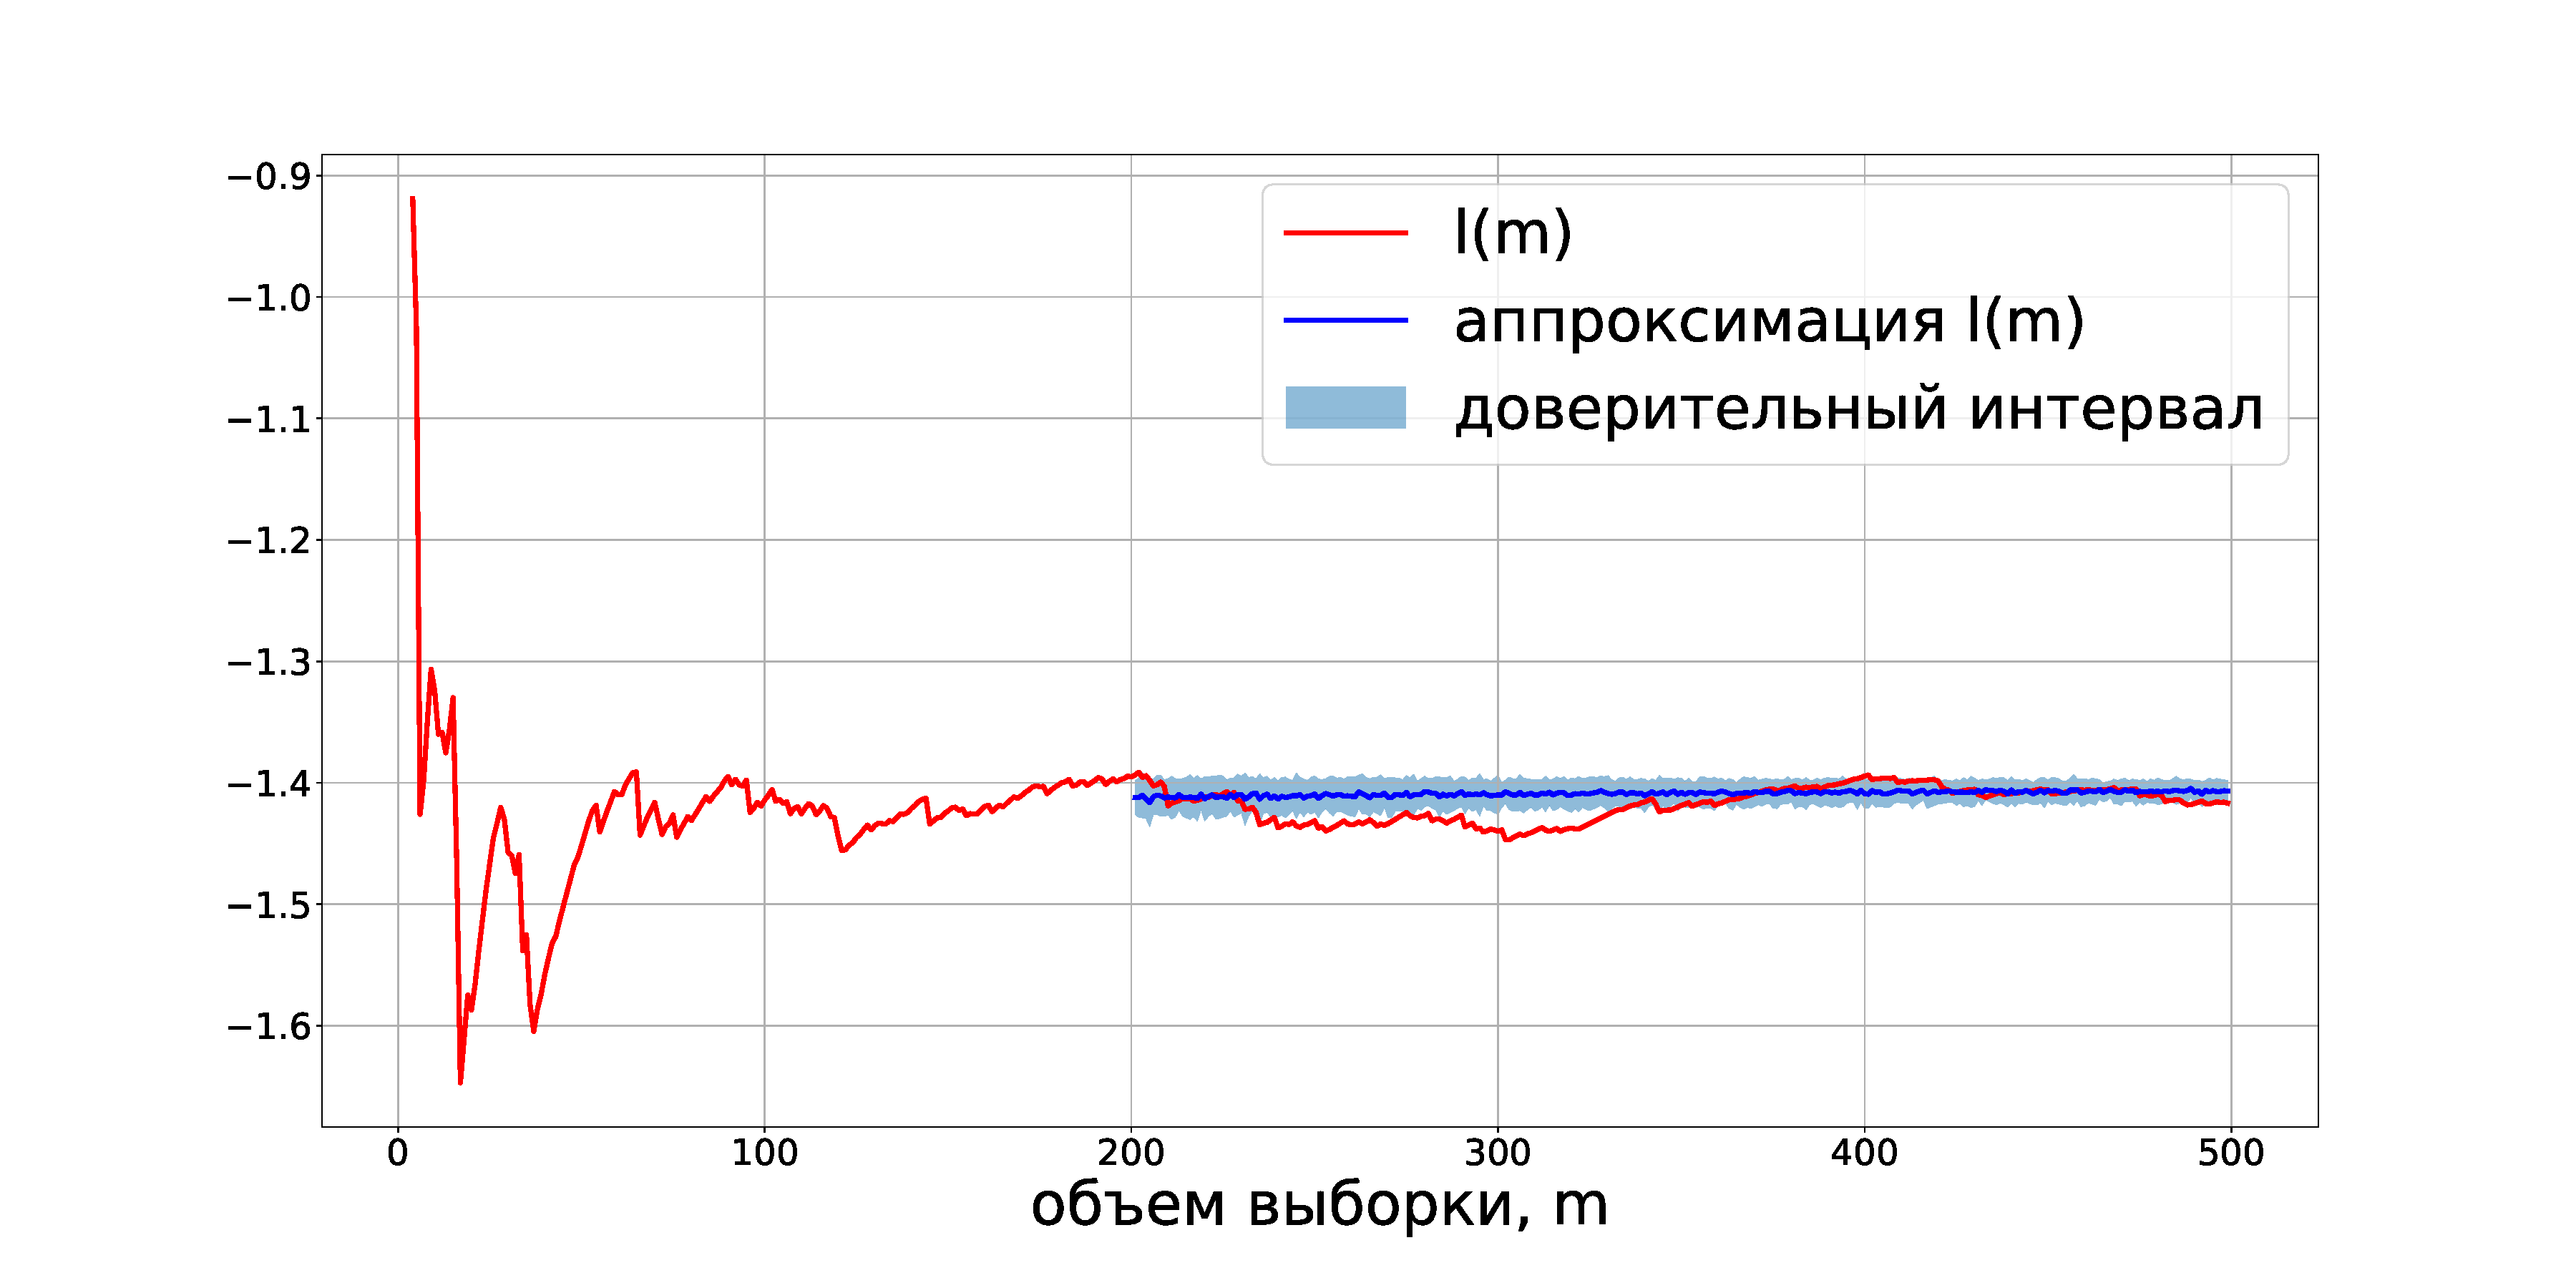
\includegraphics[width=1\textwidth]{../data/pics/synthetic_approximation_l.pdf}
%\caption{Аппроксимация функции l(m) при $m_0 = 200$}
%\label{fig4}
%\%end{figure}

%\begin{figure}[h!t]\center
%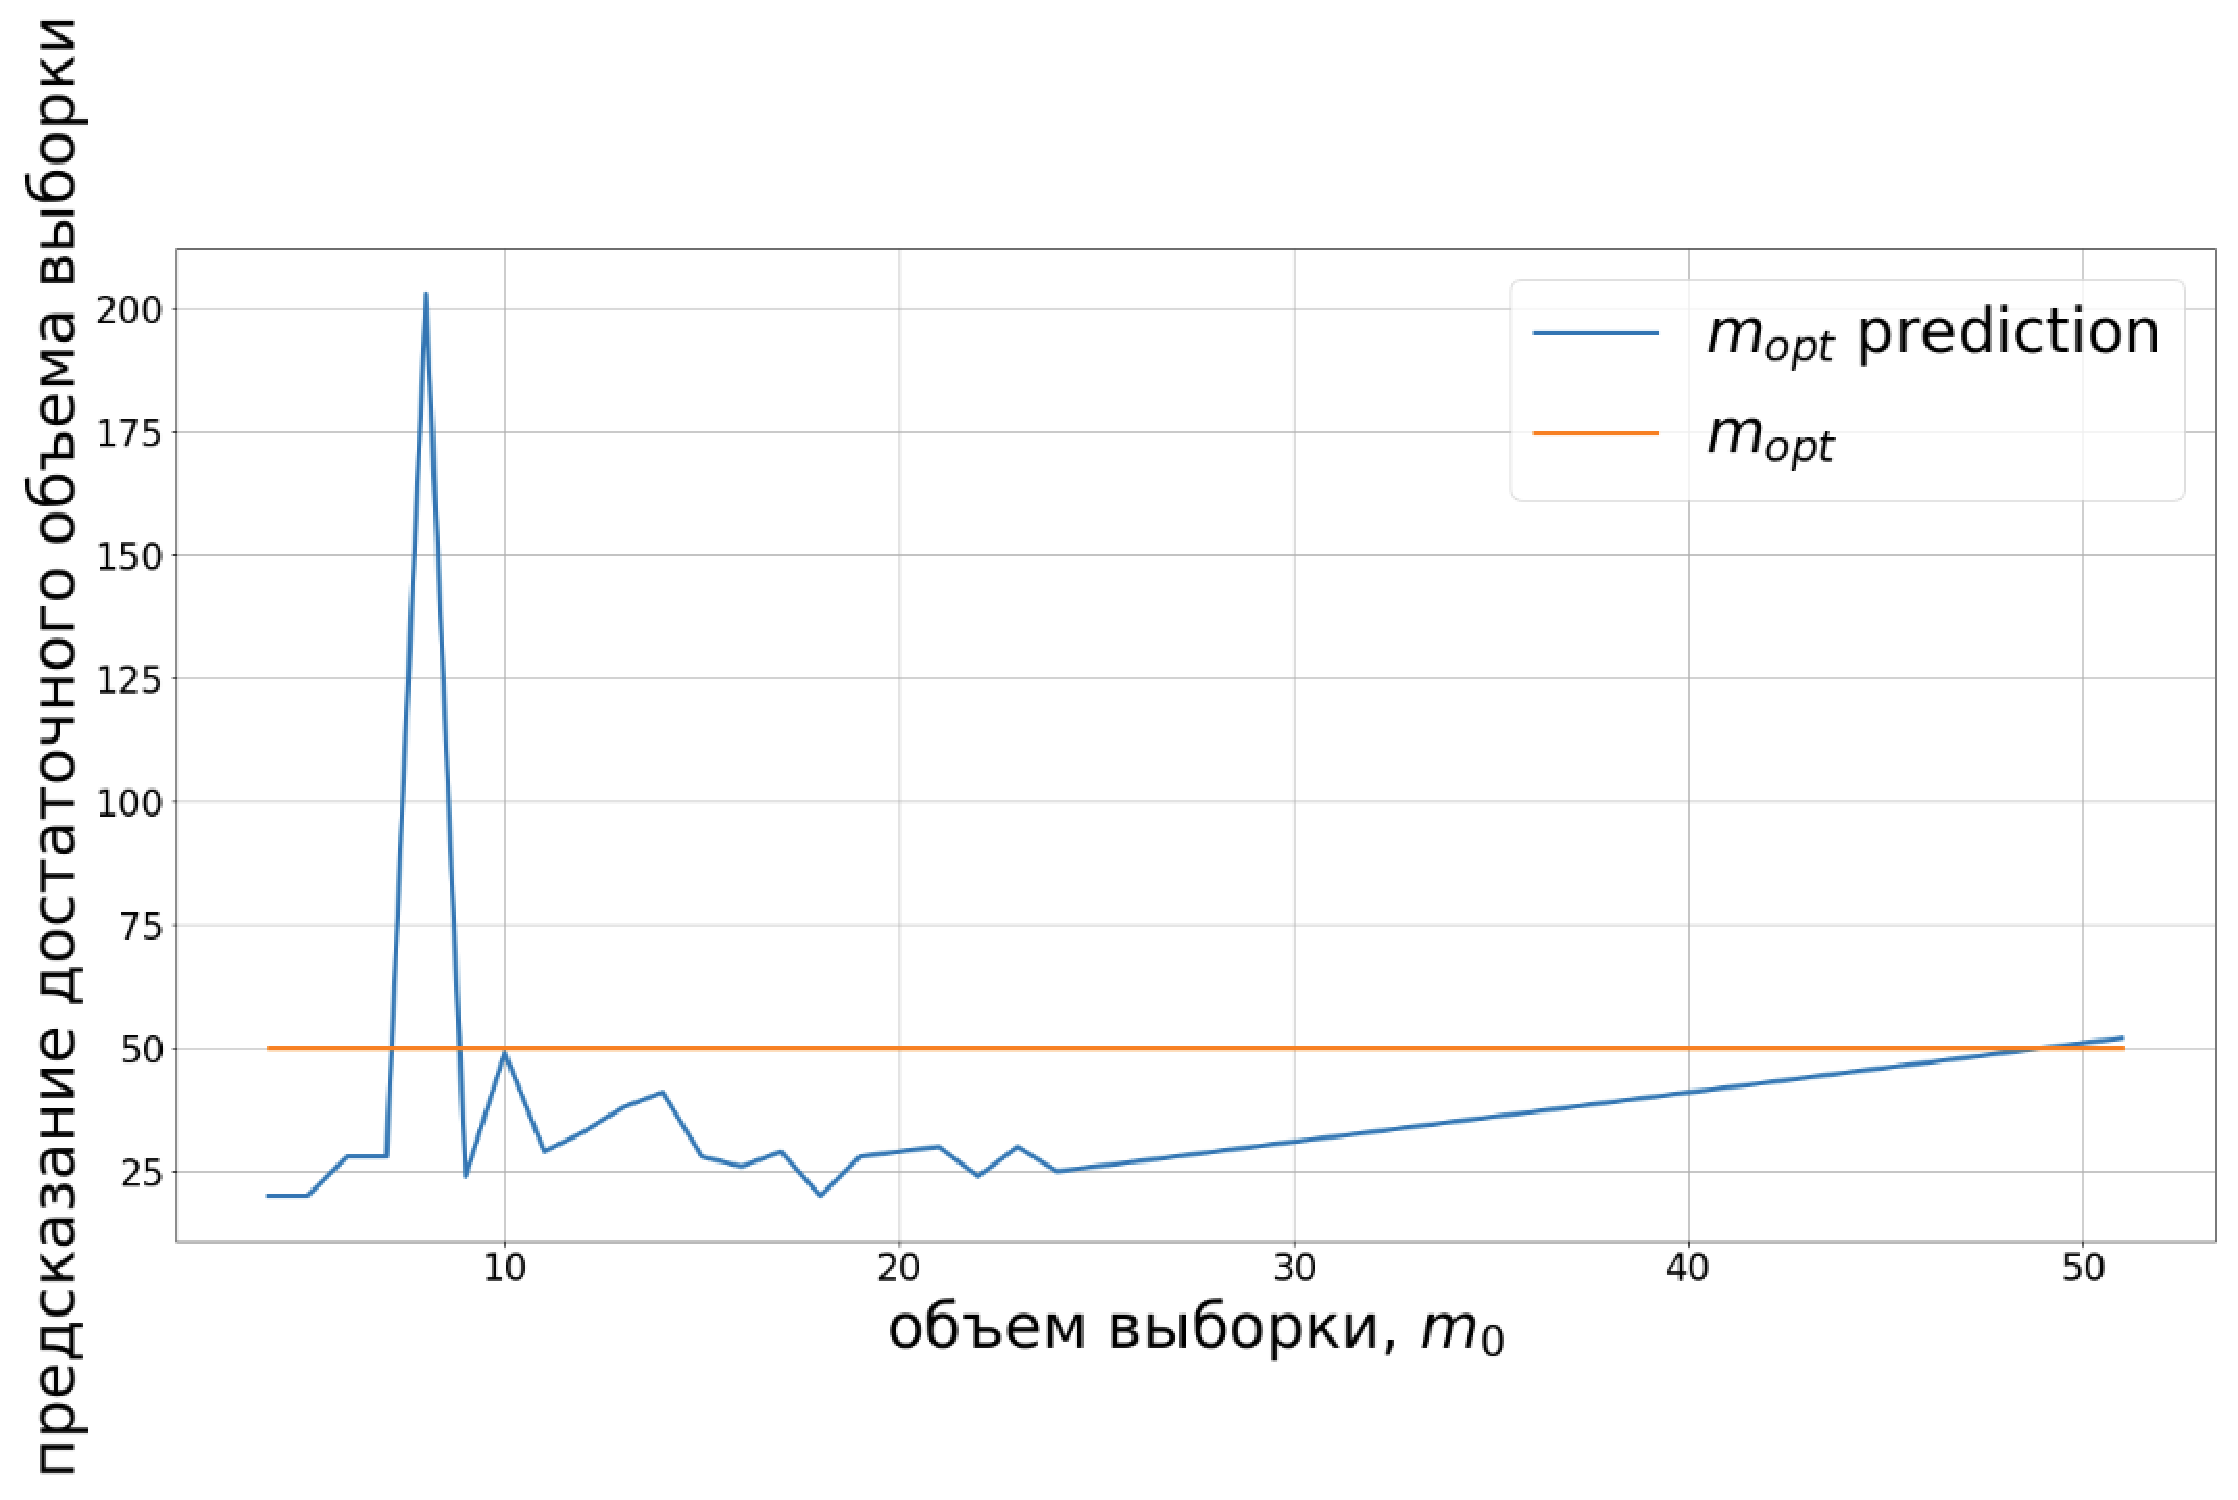
\includegraphics[width=1\textwidth]{../data/pics/synthetic_approximation_m_opt_diff.pdf}
%\caption{Аппроксимация оптимального размера выборки при разных $m_0$ (по волатильности аппроксимации функции l(m))}
%\label{fig5}
%\end{figure}


$\newline$
$\newline$
$\newline$
$\newline$
$\newline$
$\newline$
$\newline$
$\newline$
$\newline$
$\newline$

Пусть $n = 10$. Проверим, как меняется качество модели в зависимости от количества используемых признаков. Для отбора нужного количества признаков используем Лассо регрессию с функцией ошибки:

\begin{equation}\label{MSE_lasso}
MSE(\mathbf{x}, y, \textbf{w}) = \frac{1}{m}\sum\limits_{i=1}^{m}(y_i - \textbf{w}^{\top}\mathbf{x}_i )^2 + \tau \Vert \mathbf{w}\Vert_1.
\end{equation}

Используется тот факт, что Лассо регрессия обнуляет малозначимые признаки, и чем больше коэффициент $\tau$, тем больше признаков обнуляется. Таким образом можно упорядочить признаки по значимости. Для того, чтобы выбрать набор признаков $\mathcal{A}_{n^{\prime}}$ мощности $|\mathcal{A}_{n^{\prime}}| = n^{\prime}$ с наилучшей функцией ошибки, достаточно взять $n^{\prime}$ самых значимых признаков.  Для получения оценки $\hat{\mathbf{w}}$ на наборе признаков $\mathcal{A}_{n^{\prime}}$ решается оптимизационная задача (\ref{argmax_L}).

На рис. 7 построена зависимость среднего значения элементов вектора параметров $\hat{\mathbf{w}}$ от величины $\tau$ при обучении Лассо регрессии (\ref{argmax_L}), (\ref{MSE_lasso}) на подвыборках размера $m_0 = 100$.

На рис. 8, 9 построены зависимости матожидания и дисперсии функции $e^{-MSE(\mathbf{x}, y, \hat{\mathbf{w}})}$ от объёма выборки и от количества используемых признаков.


\begin{figure}[h!t]\center
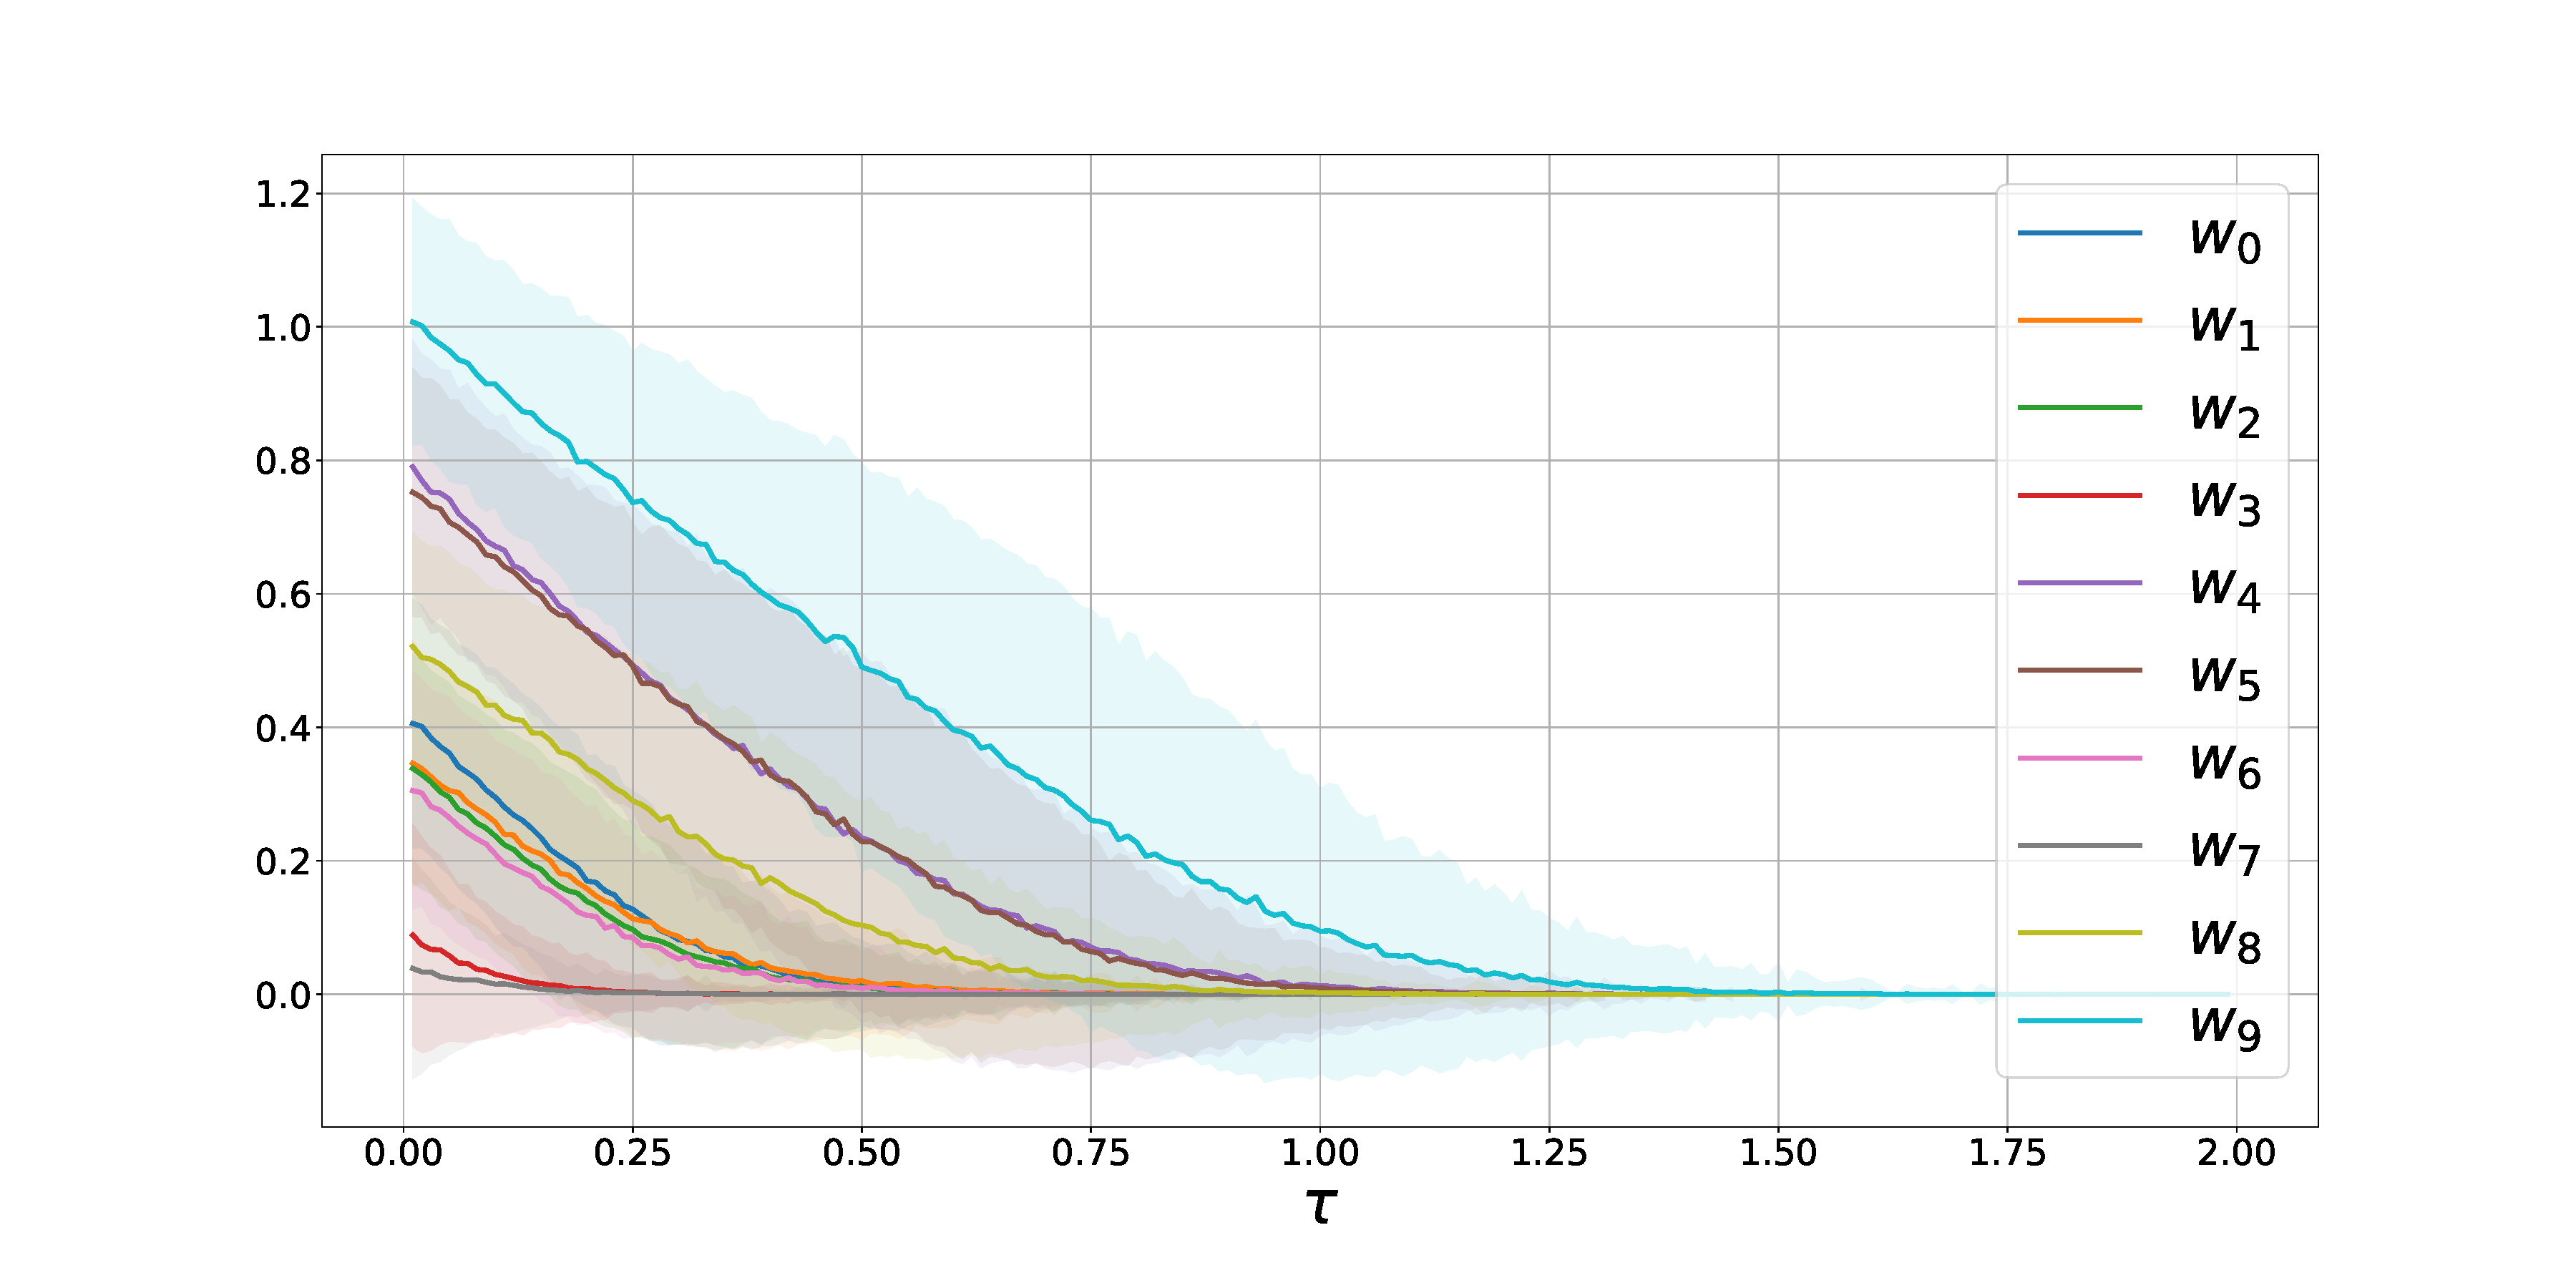
\includegraphics[width=1\textwidth]{../data/pics/synthetic_lasso_W.pdf}
\caption{Зависимость значений элементов вектора параметров от величины $\tau$}
\label{fig6}
\end{figure}

\begin{figure}[h!t]\center
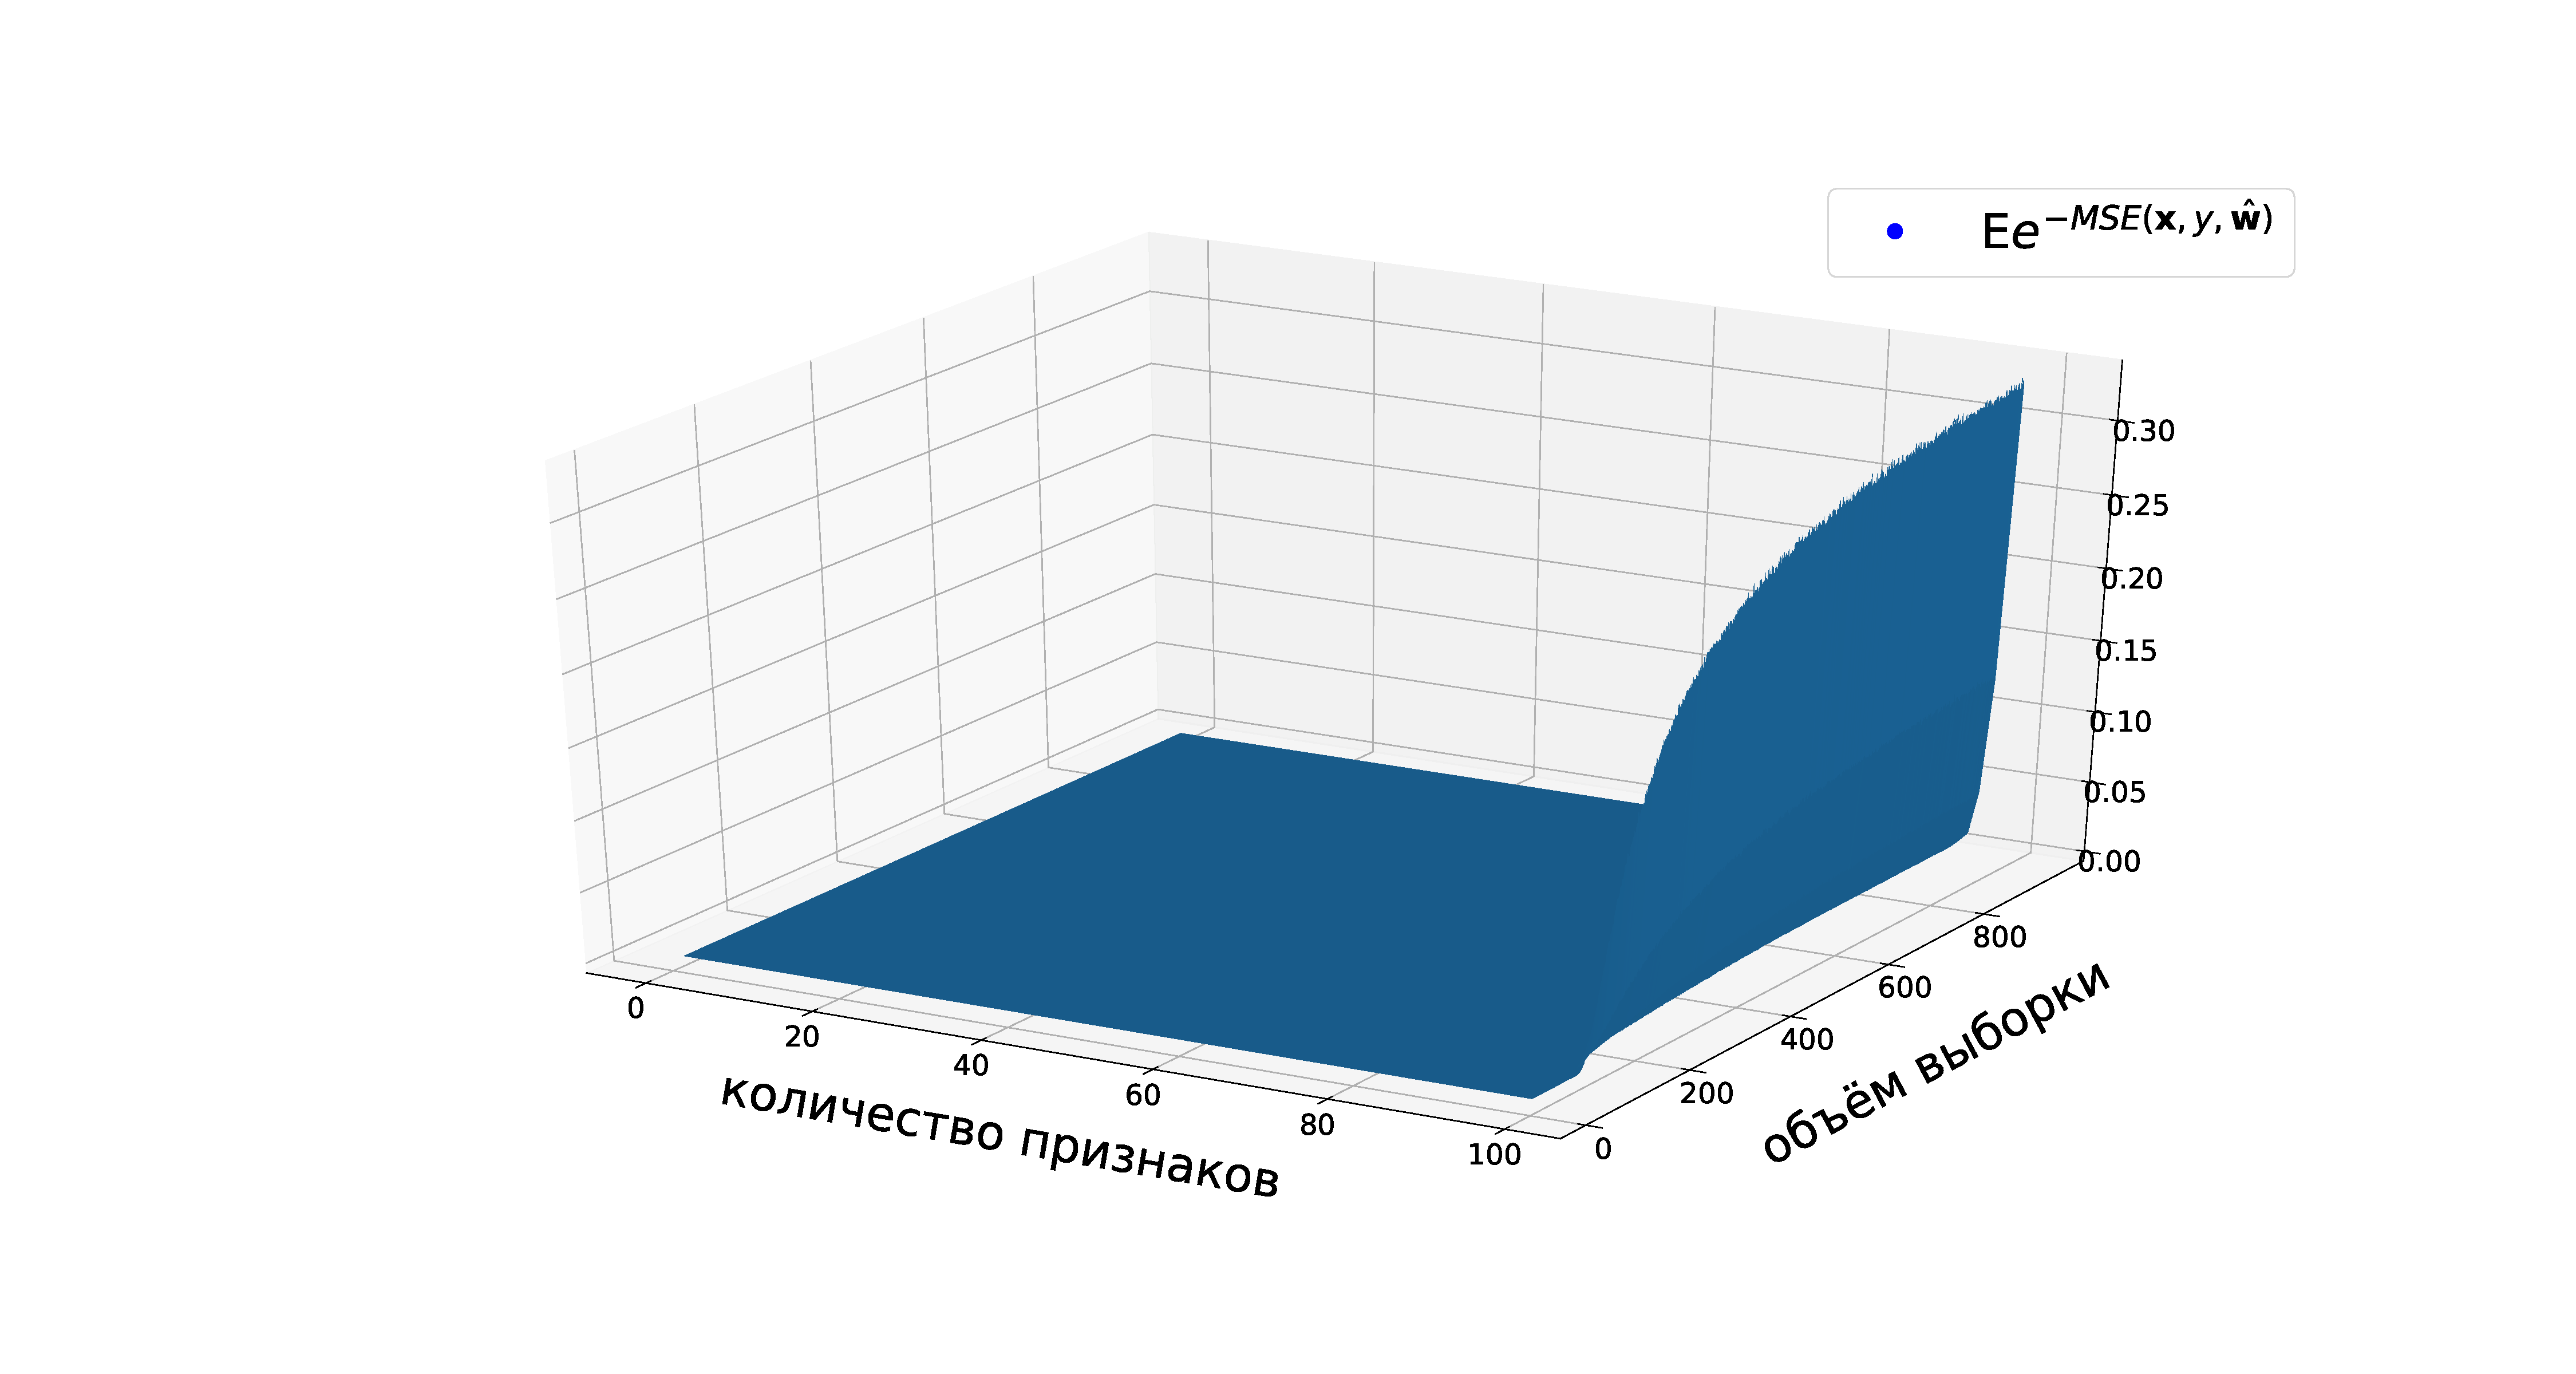
\includegraphics[width=1\textwidth]{../data/pics/synthetic_MSE_surface.pdf}
\caption{Зависимость матожидания значения $e^{-MSE(\mathbf{x}, y, \hat{\mathbf{w}})}$ от объёма выборки и от количества используемых признаков}
\label{fig7}
\end{figure}

\begin{figure}[h!t]\center
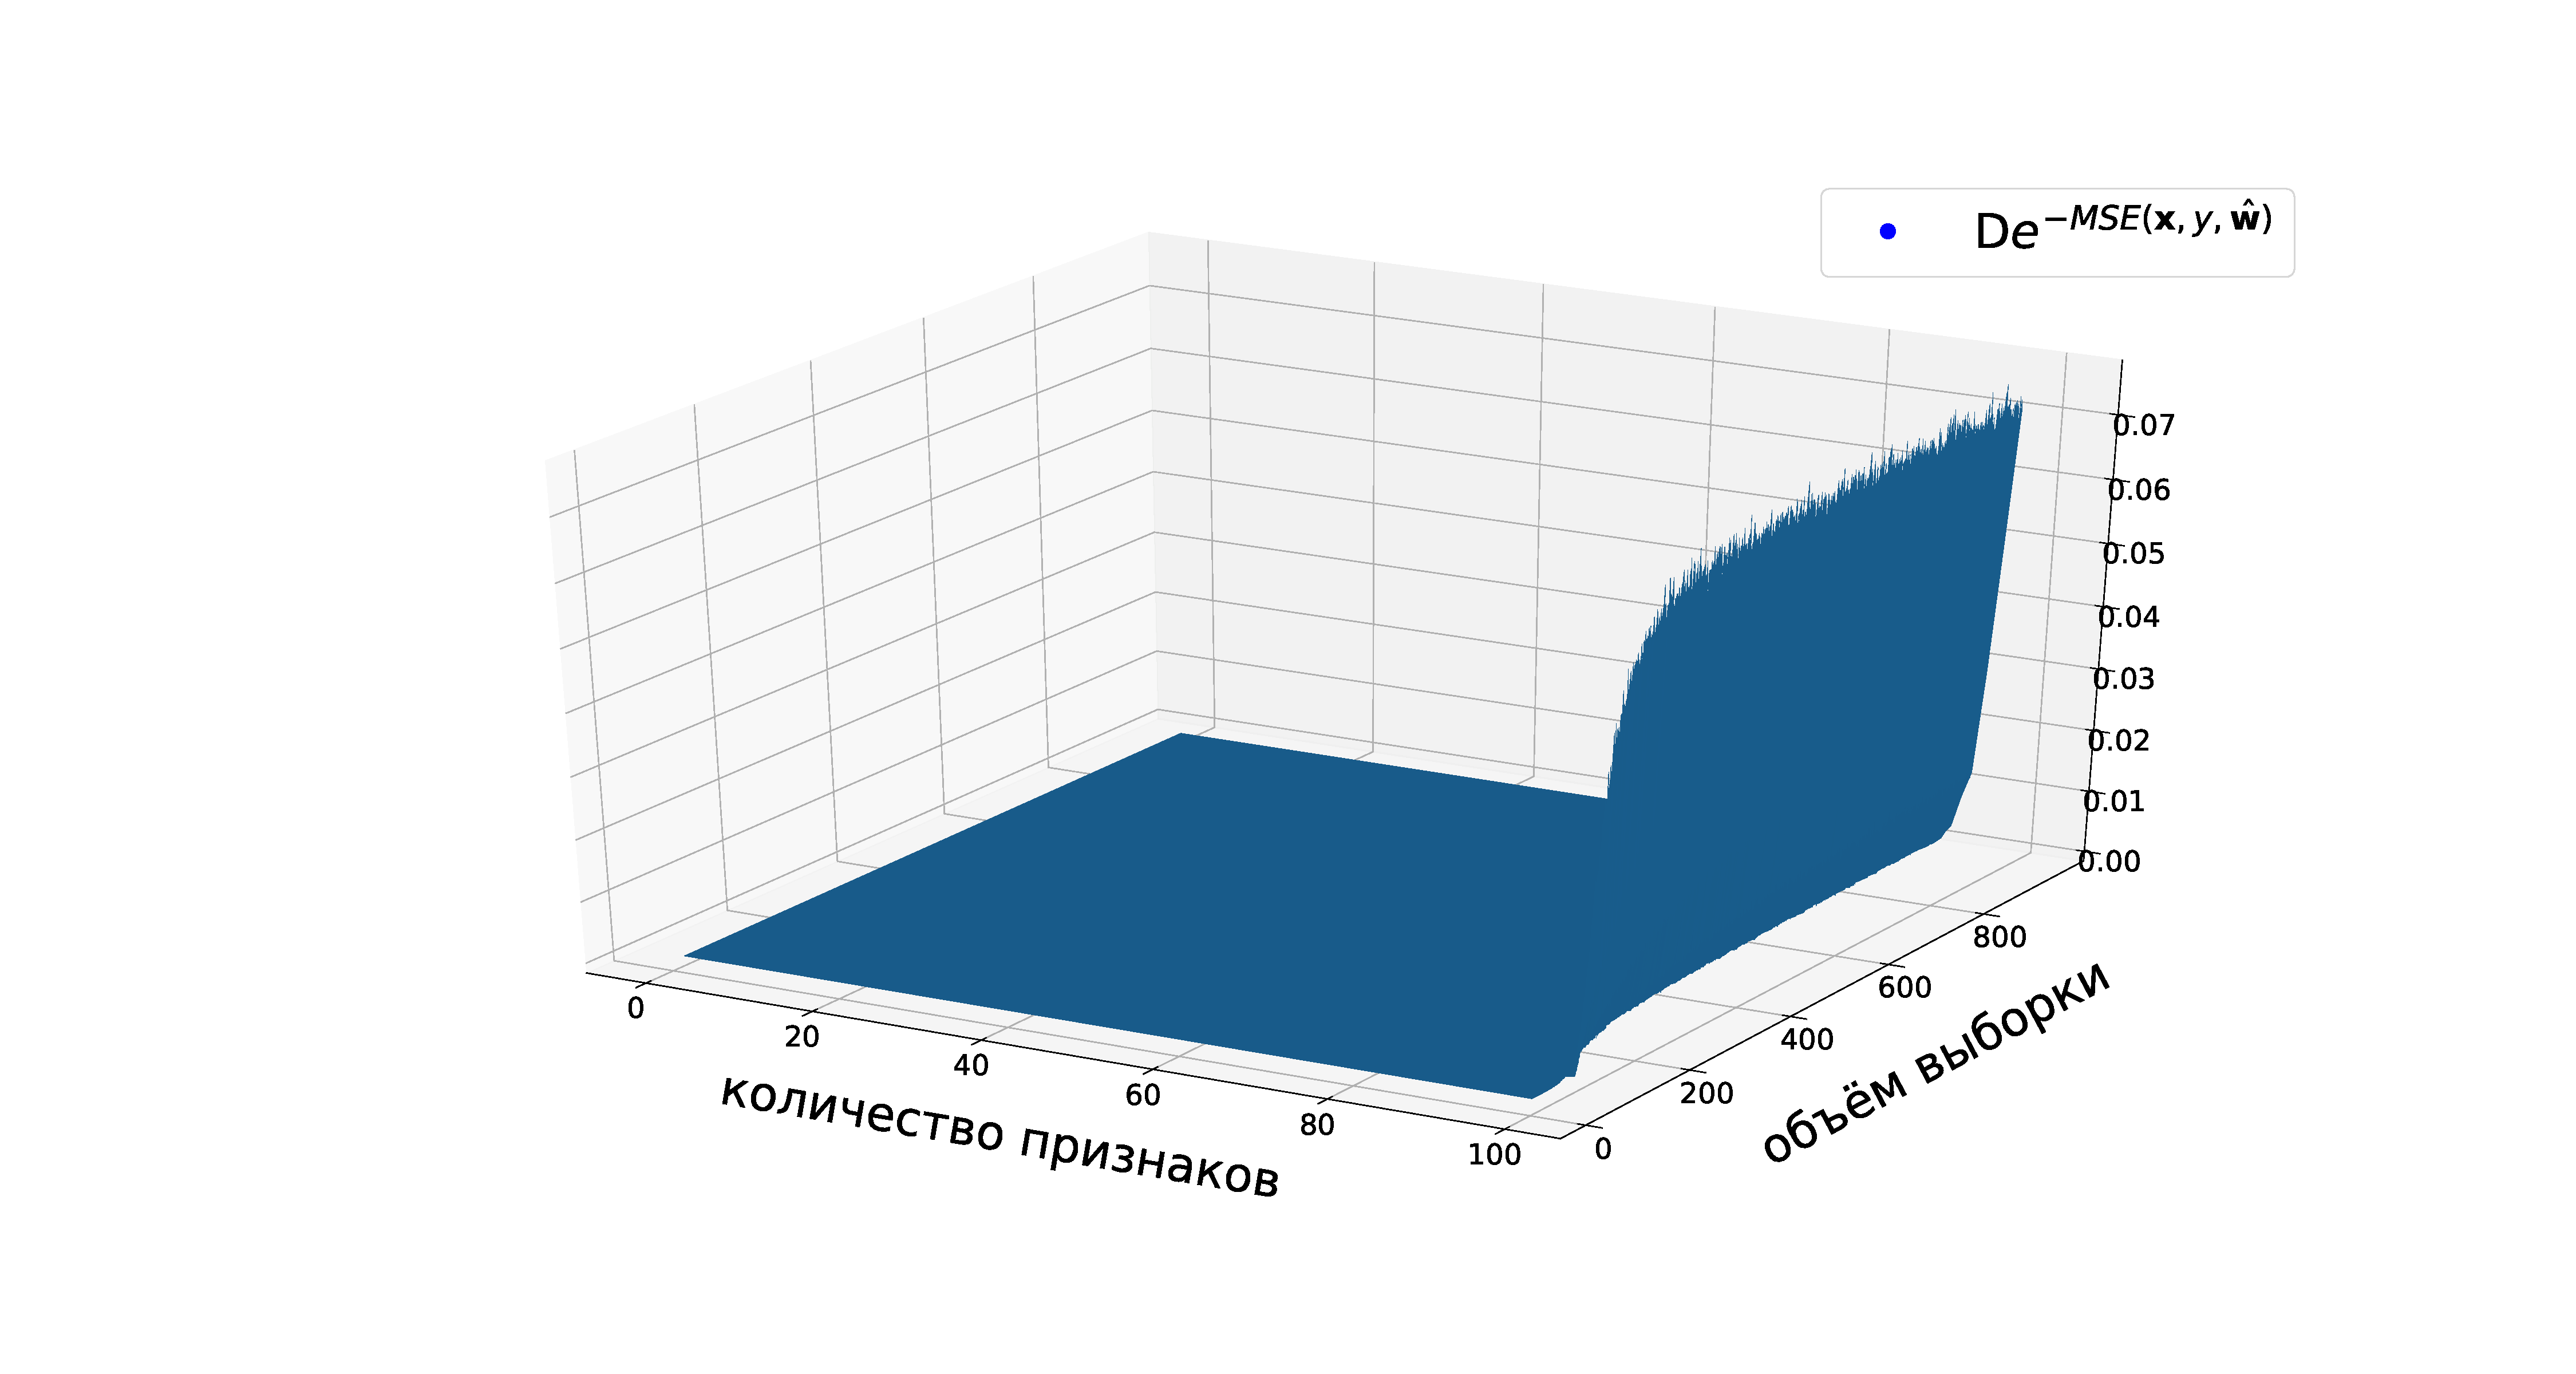
\includegraphics[width=1\textwidth]{../data/pics/synthetic_MSE_std_surface.pdf}
\caption{Зависимость дисперсии значения $e^{-MSE(\mathbf{x}, y, \hat{\mathbf{w}})}$ от объёма выборки и от количества используемых признаков}
\label{fig8}
\end{figure}


$\newline$
$\newline$
$\newline$
$\newline$
$\newline$
$\newline$
$\newline$
$\newline$
$\newline$
$\newline$

На рис. 10 построена зависимость значения элементов оценки ковариационной матрицы параметров $\hat{A}$ от количества используемых признаков $n^{\prime}$ при обучении модели линейной регрессии (\ref{argmax_L}), (\ref{MSE}). Можно заметить, что ковариация между парой признаков $\mathbf{w}_i, \mathbf{w}_j$, попавших в набор используемых признаков $\mathcal{A}_{n^{\prime}}$, слабо зависит от $n^{\prime}$ и остается практически неизменной.

На рис. 11 построена зависимость значения элементов оценки ковариационной матрицы параметров $\hat{A}$ от коэффициента регуляризации $\tau$ при обучении Лассо регрессии (\ref{argmax_MSE}), (\ref{MSE_lasso}). Можно заметить, что ковариация $cov(\mathbf{w}_i, \mathbf{w}_j)$ обратно пропорциональна величине $\tau$.

\begin{figure}[h!t]\center
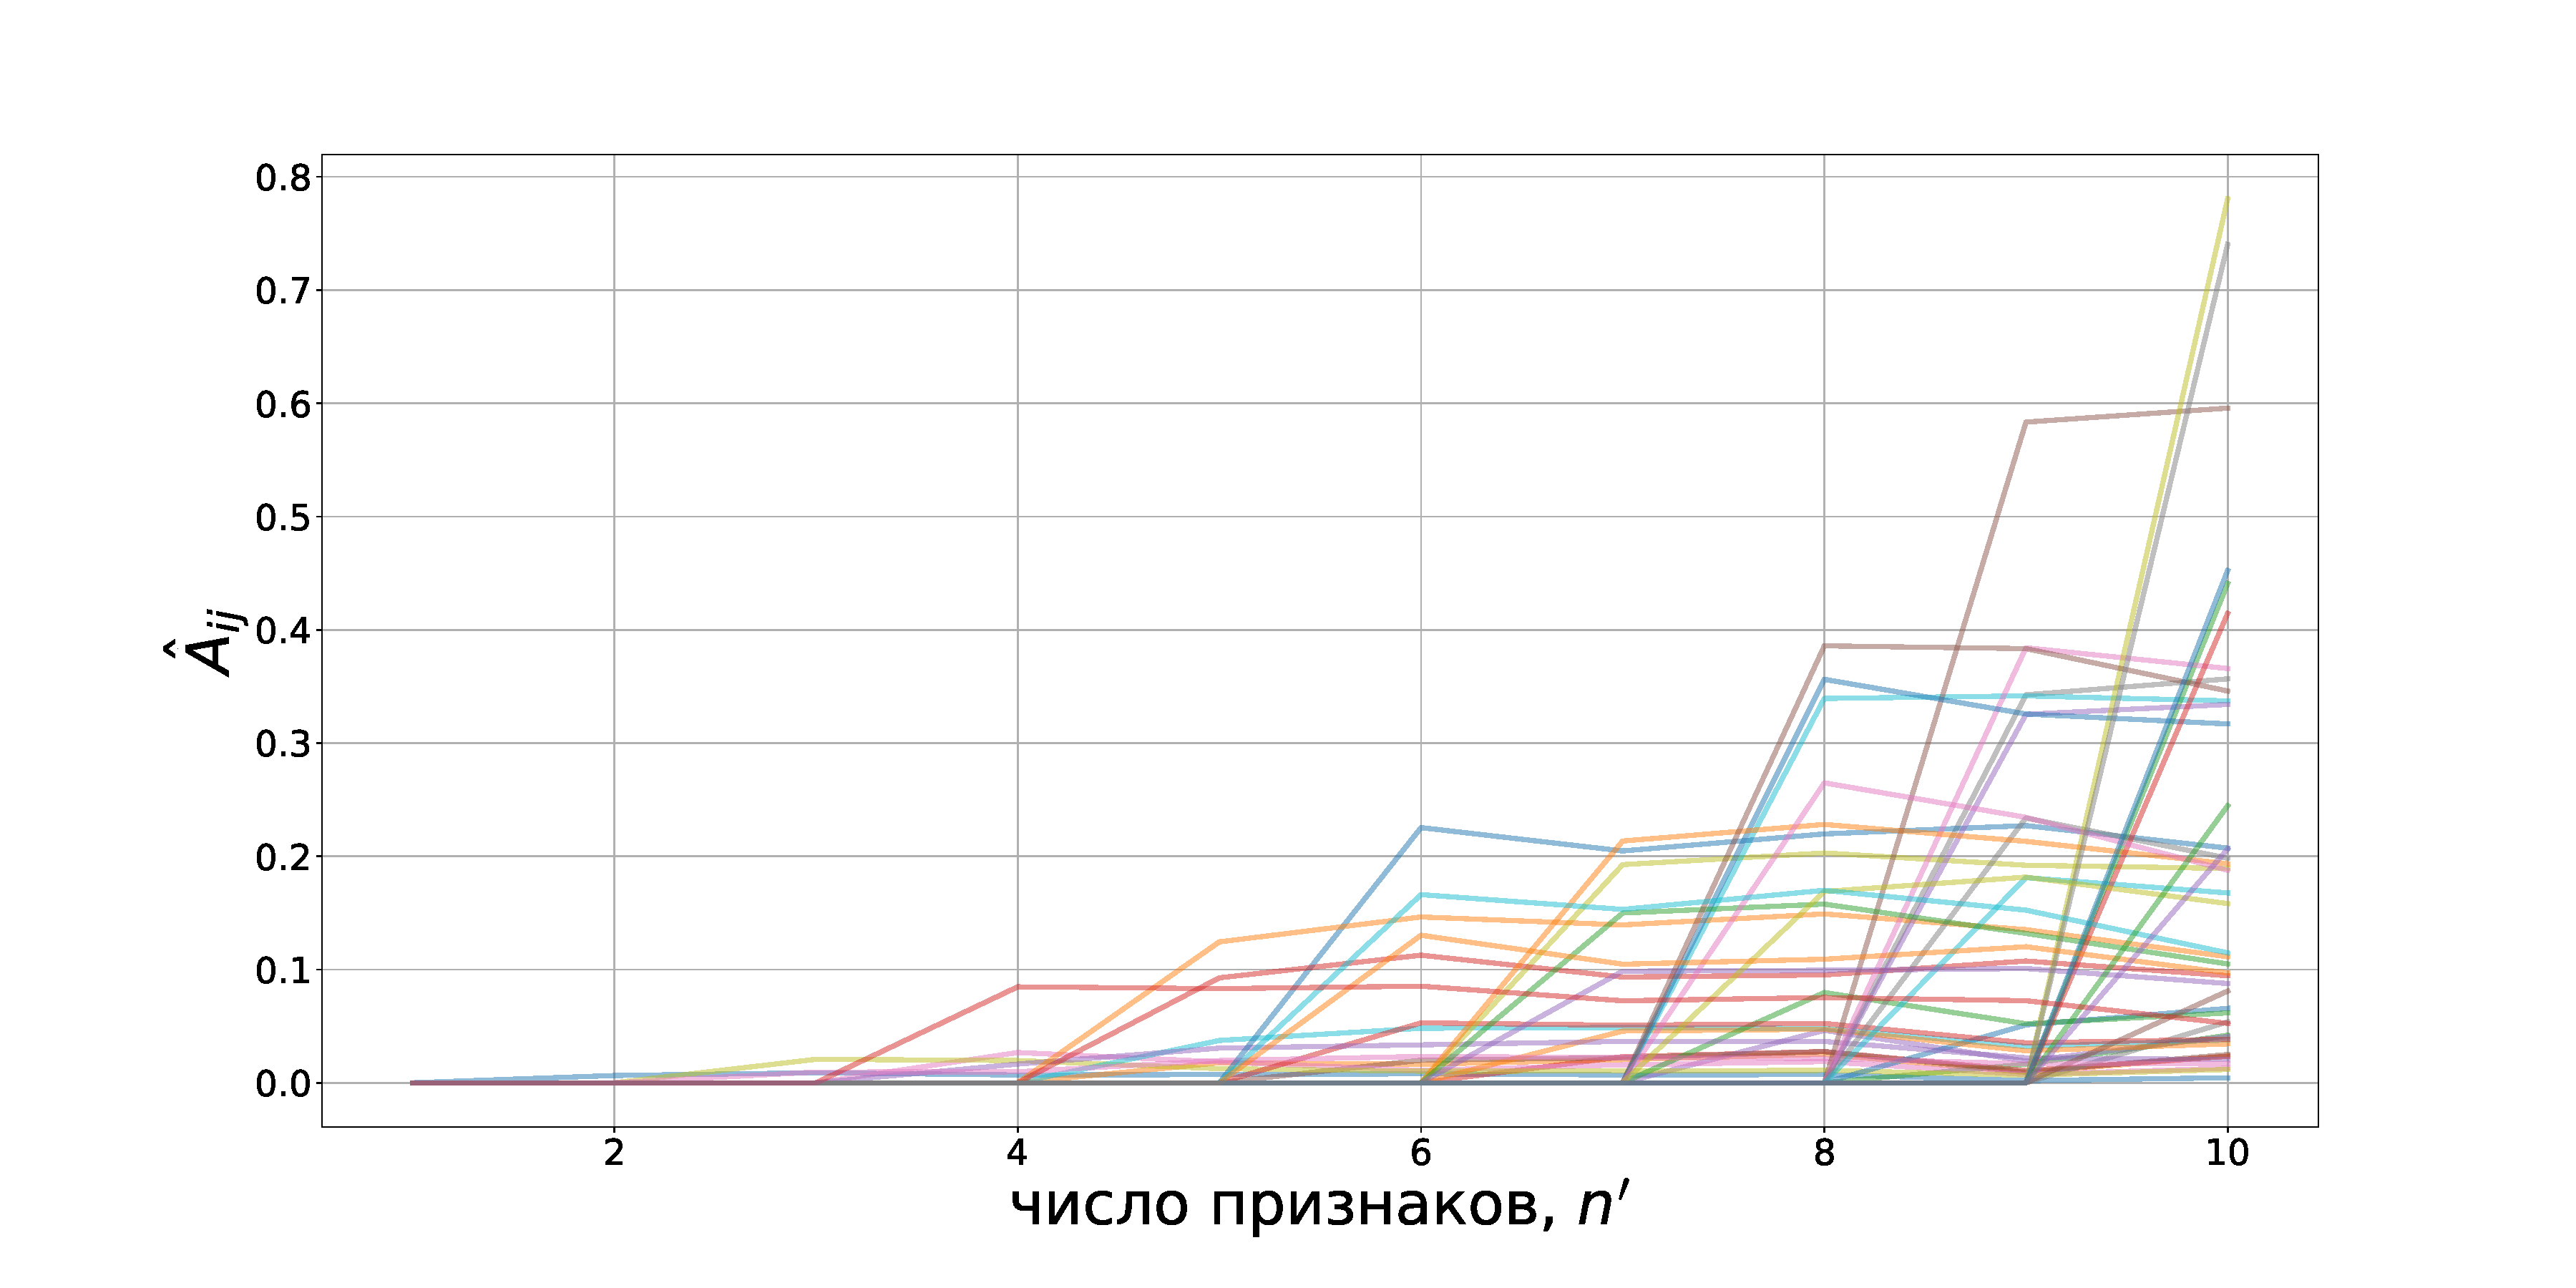
\includegraphics[width=1\textwidth]{../data/pics/synthetic_W_from_N.pdf}
\caption{Зависимость значения элементов ковариационной матрицы $\hat{A}$ от числа используемых признаков $n$, $m = 100$.}
\label{fig9}
\end{figure}

\begin{figure}[h!t]\center
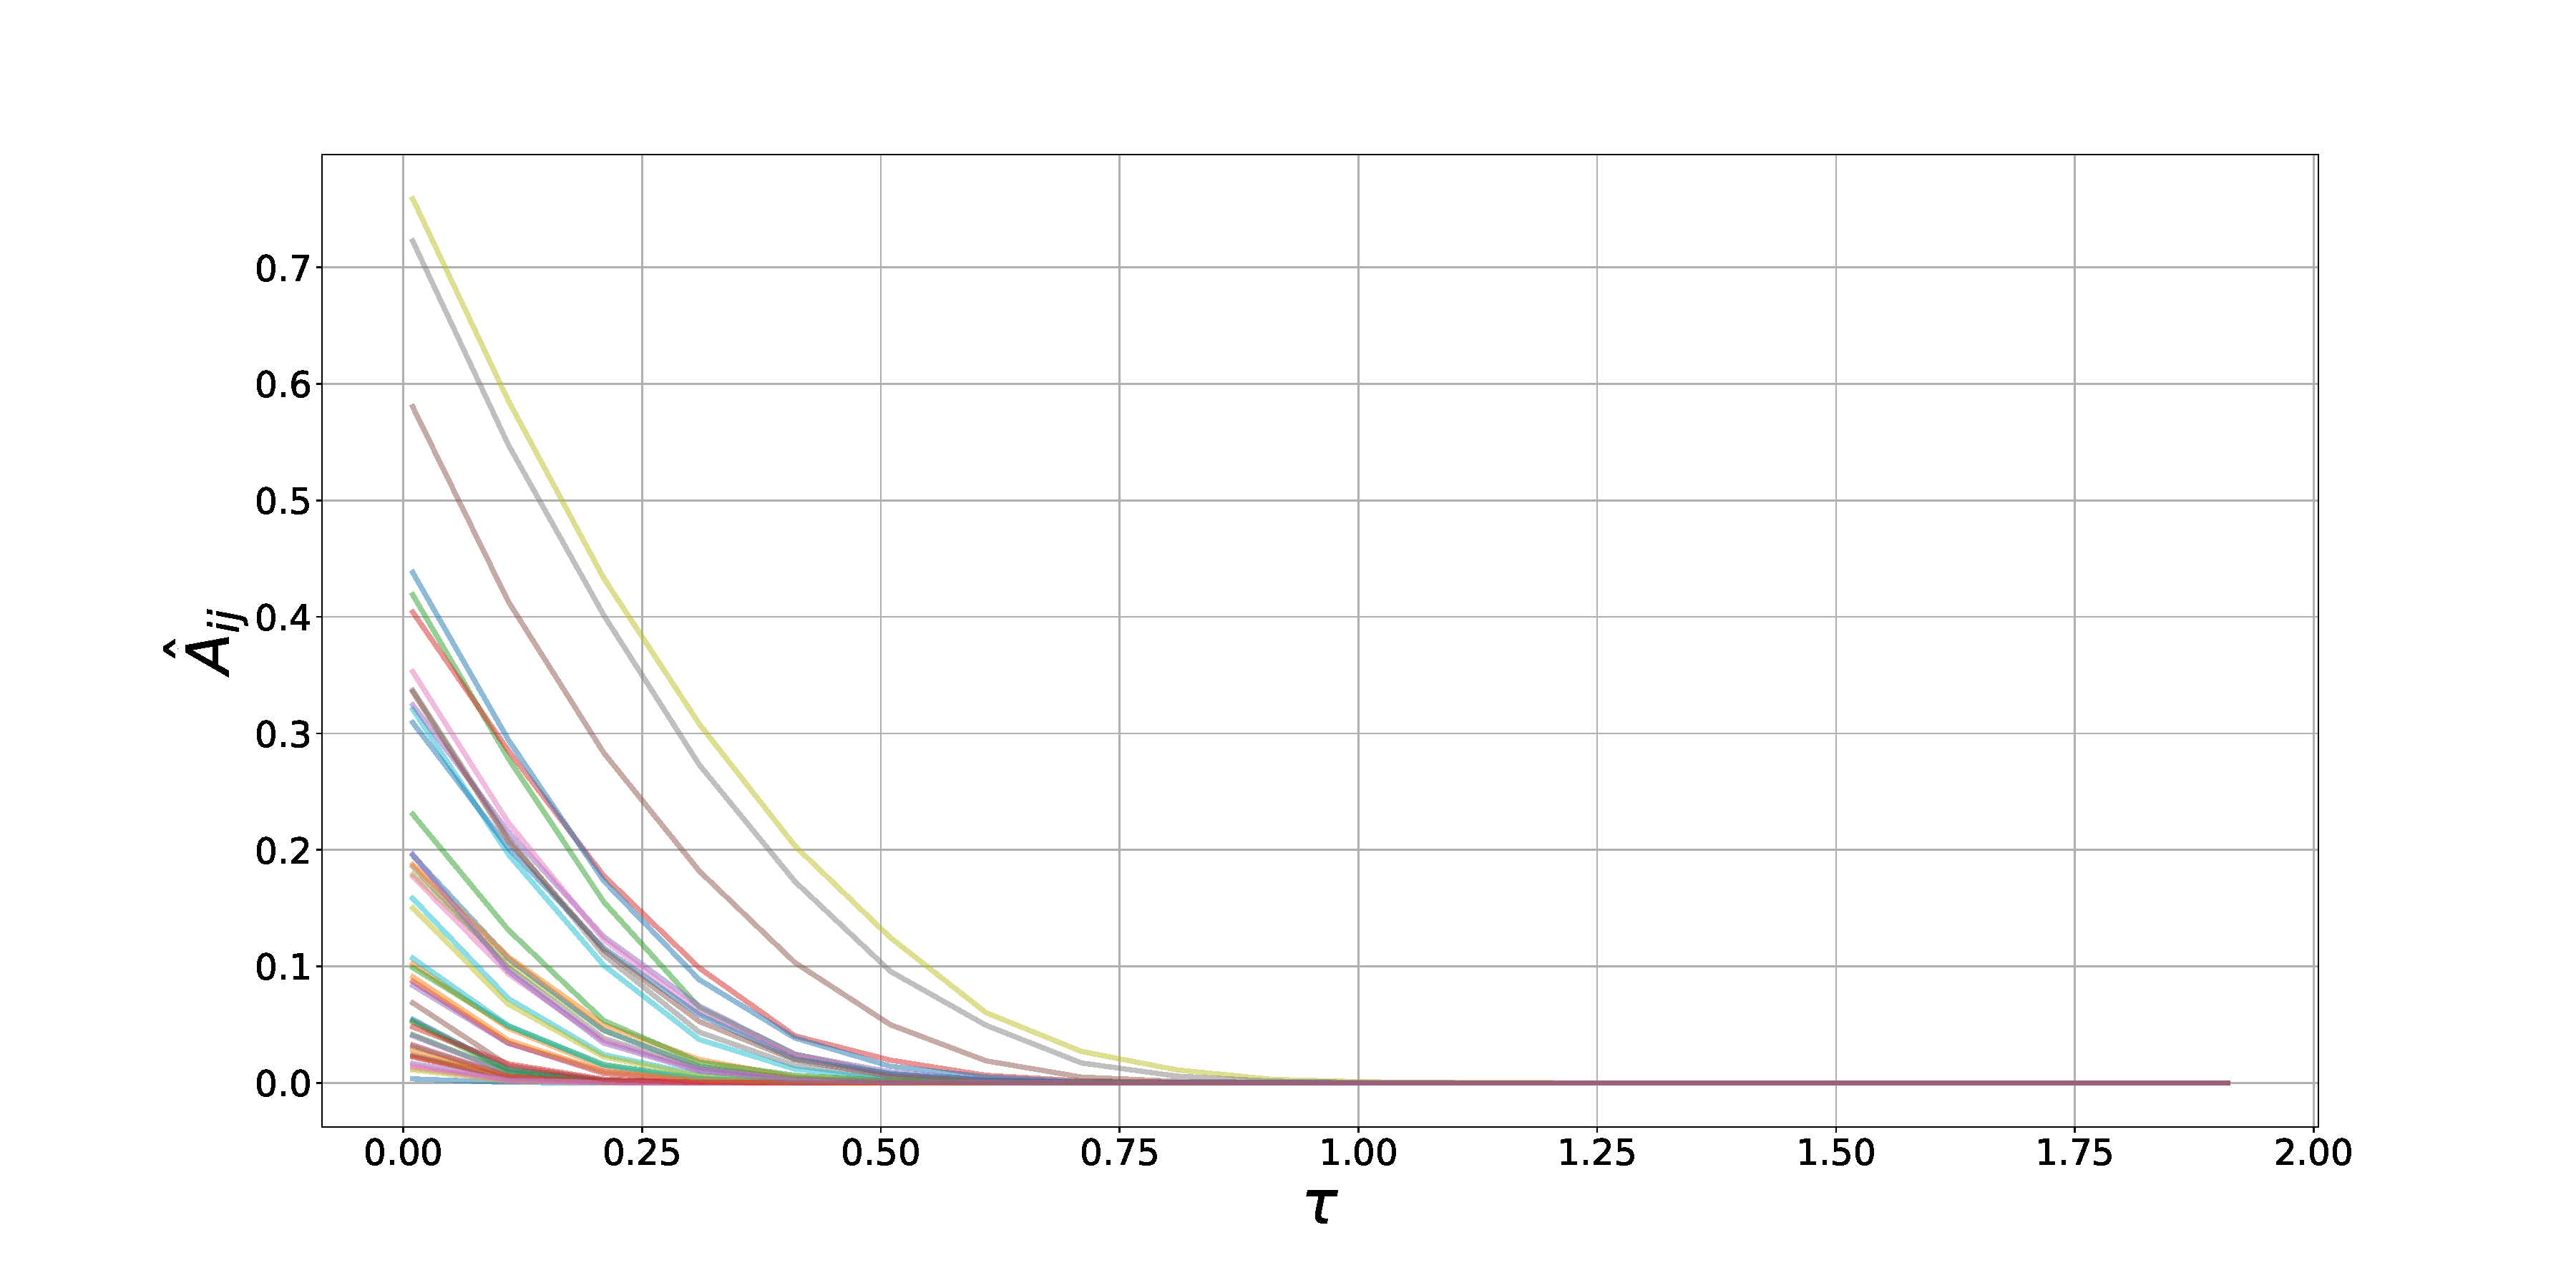
\includegraphics[width=1\textwidth]{../data/pics/synthetic_W_from_tau.pdf}
\caption{Зависимость значения элементов ковариационной матрицы $\hat{A}$ от коэффициента $\tau$, $m = 100$.}
\label{fig10}
\end{figure}


$\newline$
$\newline$
$\newline$
$\newline$
$\newline$
$\newline$
$\newline$
$\newline$
$\newline$
$\newline$
$\newline$
$\newline$
$\newline$
$\newline$
$\newline$
$\newline$


\section{Вычислительный эксперимент}

Для анализа точности и эффективности предлагаемого метода был проведен вычислительный эксперимент. В качестве данных использовались выборки, описанные в таблице 1.

\begin{table}[h!]
\begin{center}
\caption{Описание выборок}
\label{table1}
\begin{tabularx}{\textwidth}{|p{1in}|X|X|c|}
\hline
	\centering Выборка &\centeringТип задачи&\centering Размер выборки& Число признаков\\
	\hline
	Servo &регрессия&\centering167&4\\
	\hline
	Boston &регрессия&\centering506&13\\
	\hline
	Diabetes&регрессия&\centering 442&5\\
\hline
\end{tabularx}
\end{center}
\end{table}

В ходе эксперимента были модифицированы критерии средней длины и среднего покрытия для линейной регрессии, а именно была построена аппроксимация функции эффективности при большем объеме выборки при помощи аппроксимации ковариационной матрицы вектора параметров через матрицу информации Фишера.

На графике 1 показана зависимость значения функции эффективности от объема выборки для разных методов при разных данных. Синим цветом обозначено посчитанное значение при данном объеме, красным - аппроксимация при подвыборке фиксированного размера. Реальное значение функции эффективности попадает в доверительный интервал, что говорит о работоспособности предлагаемого метода.

\begin{figure}[h!t]\center
\centering\begin{tabular}{@{}c@{ }c@{ }c@{}}
\textbf{ALC метод} & \textbf{ACC метод}\\
\subfloat[Servo]{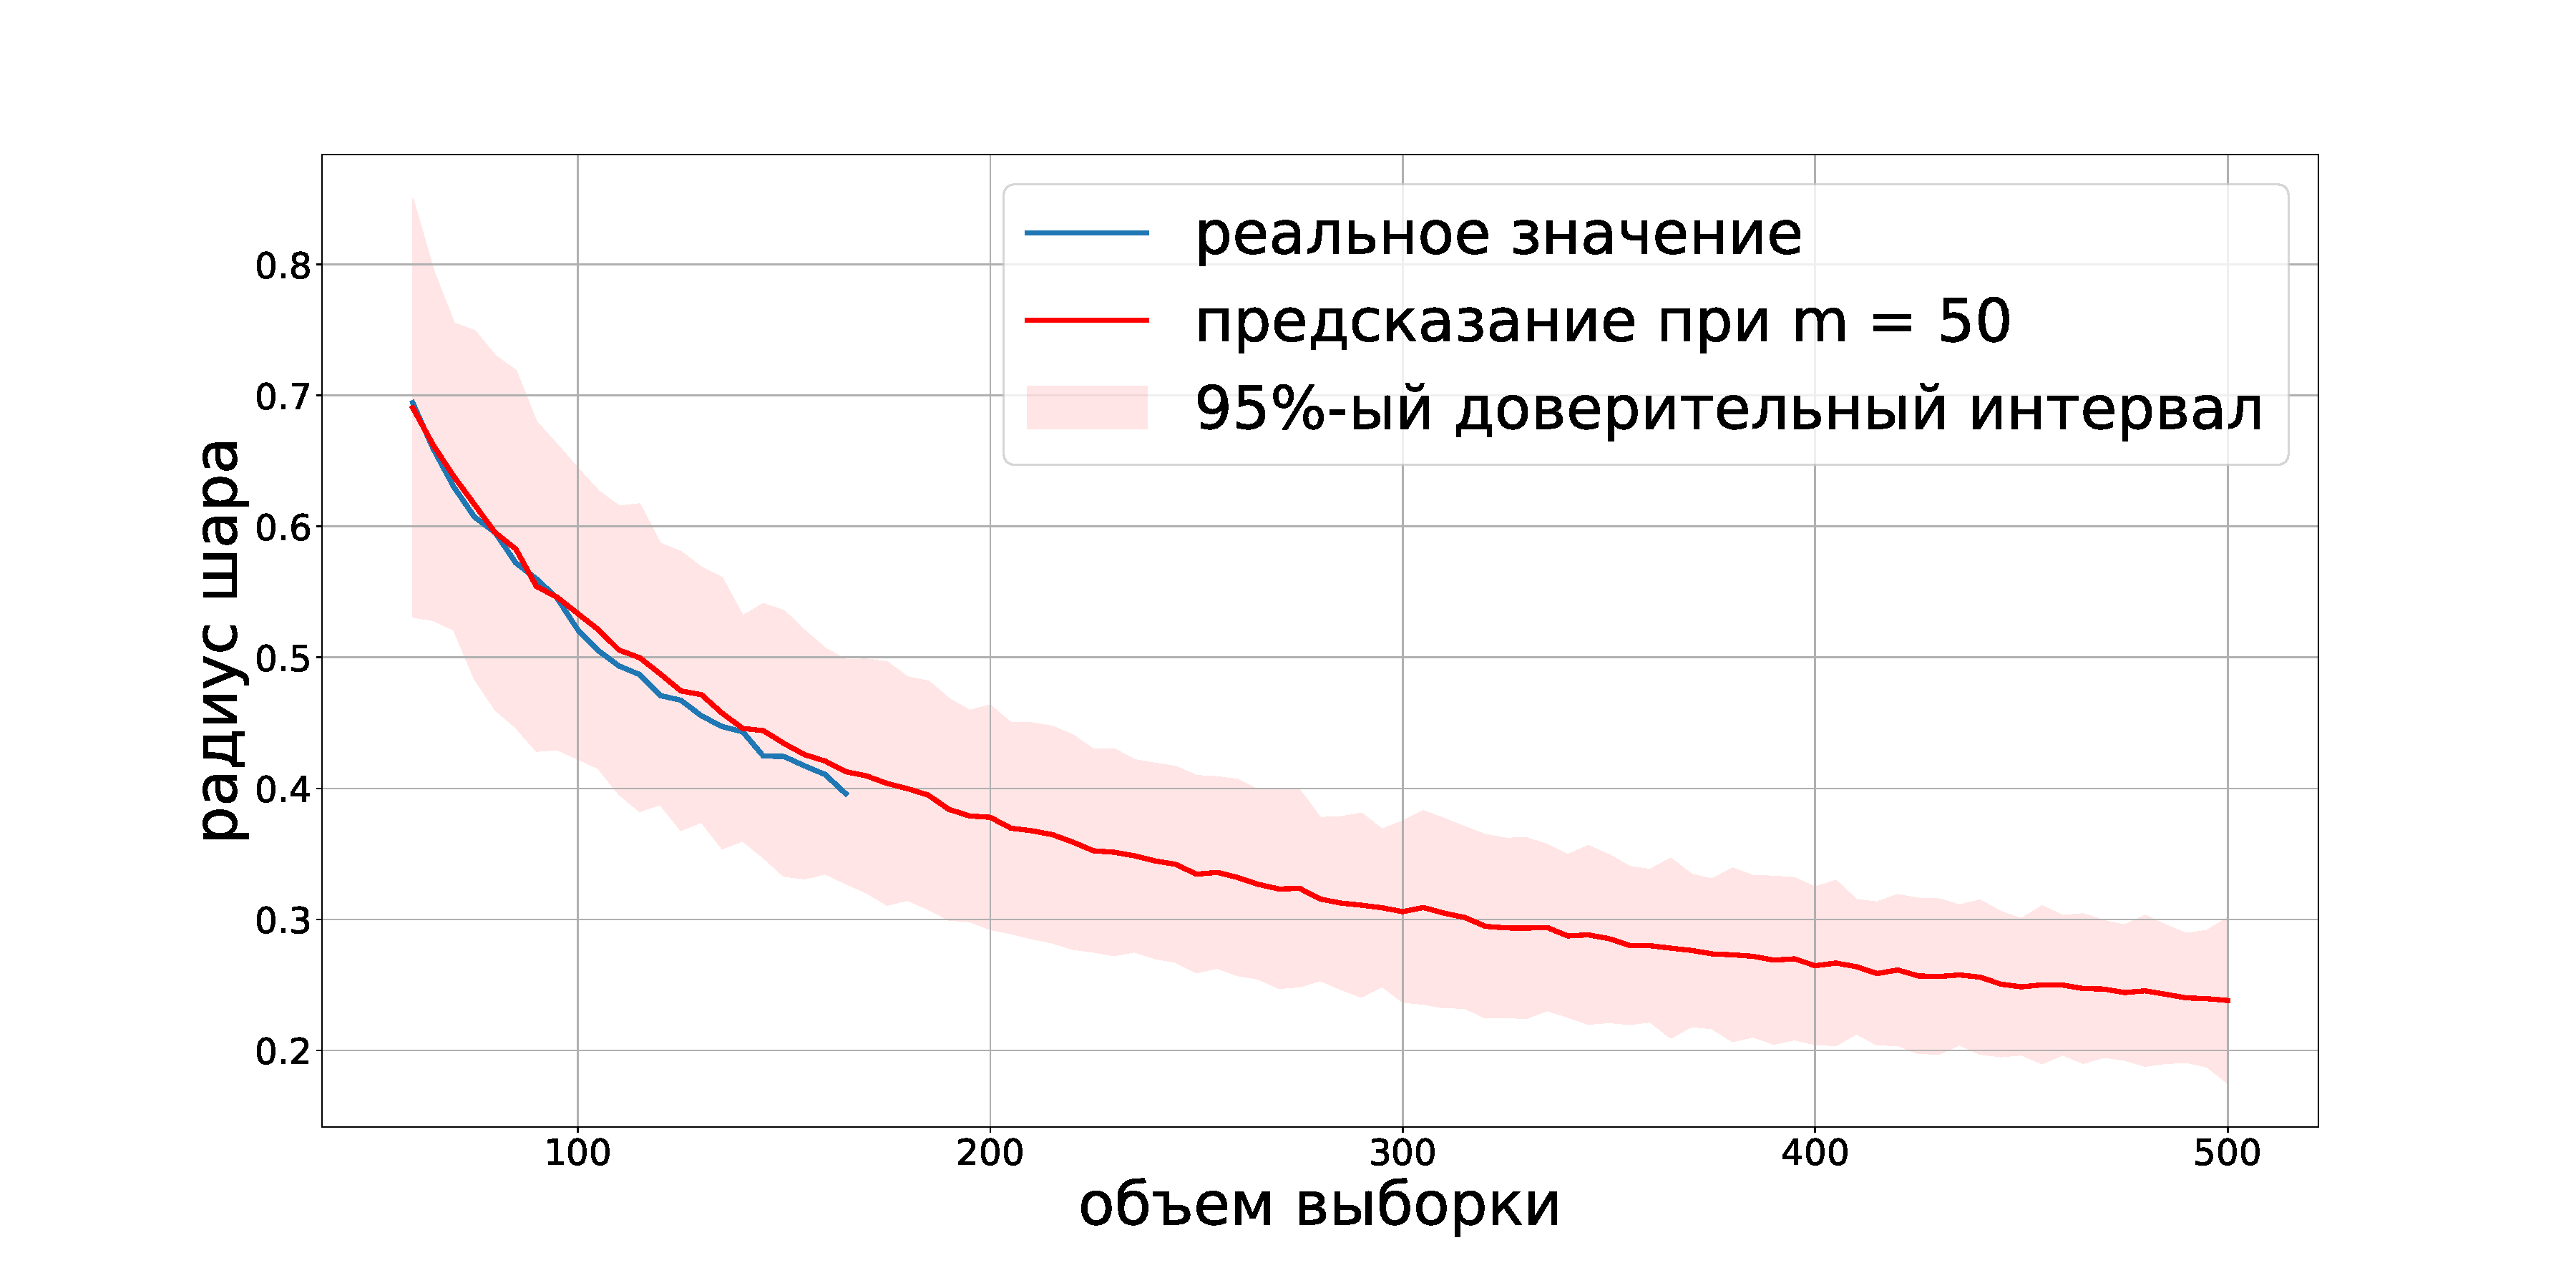
\includegraphics[width=0.5\textwidth]{../data/pics/ALC_modified_servo.pdf}}&
\subfloat[Servo]{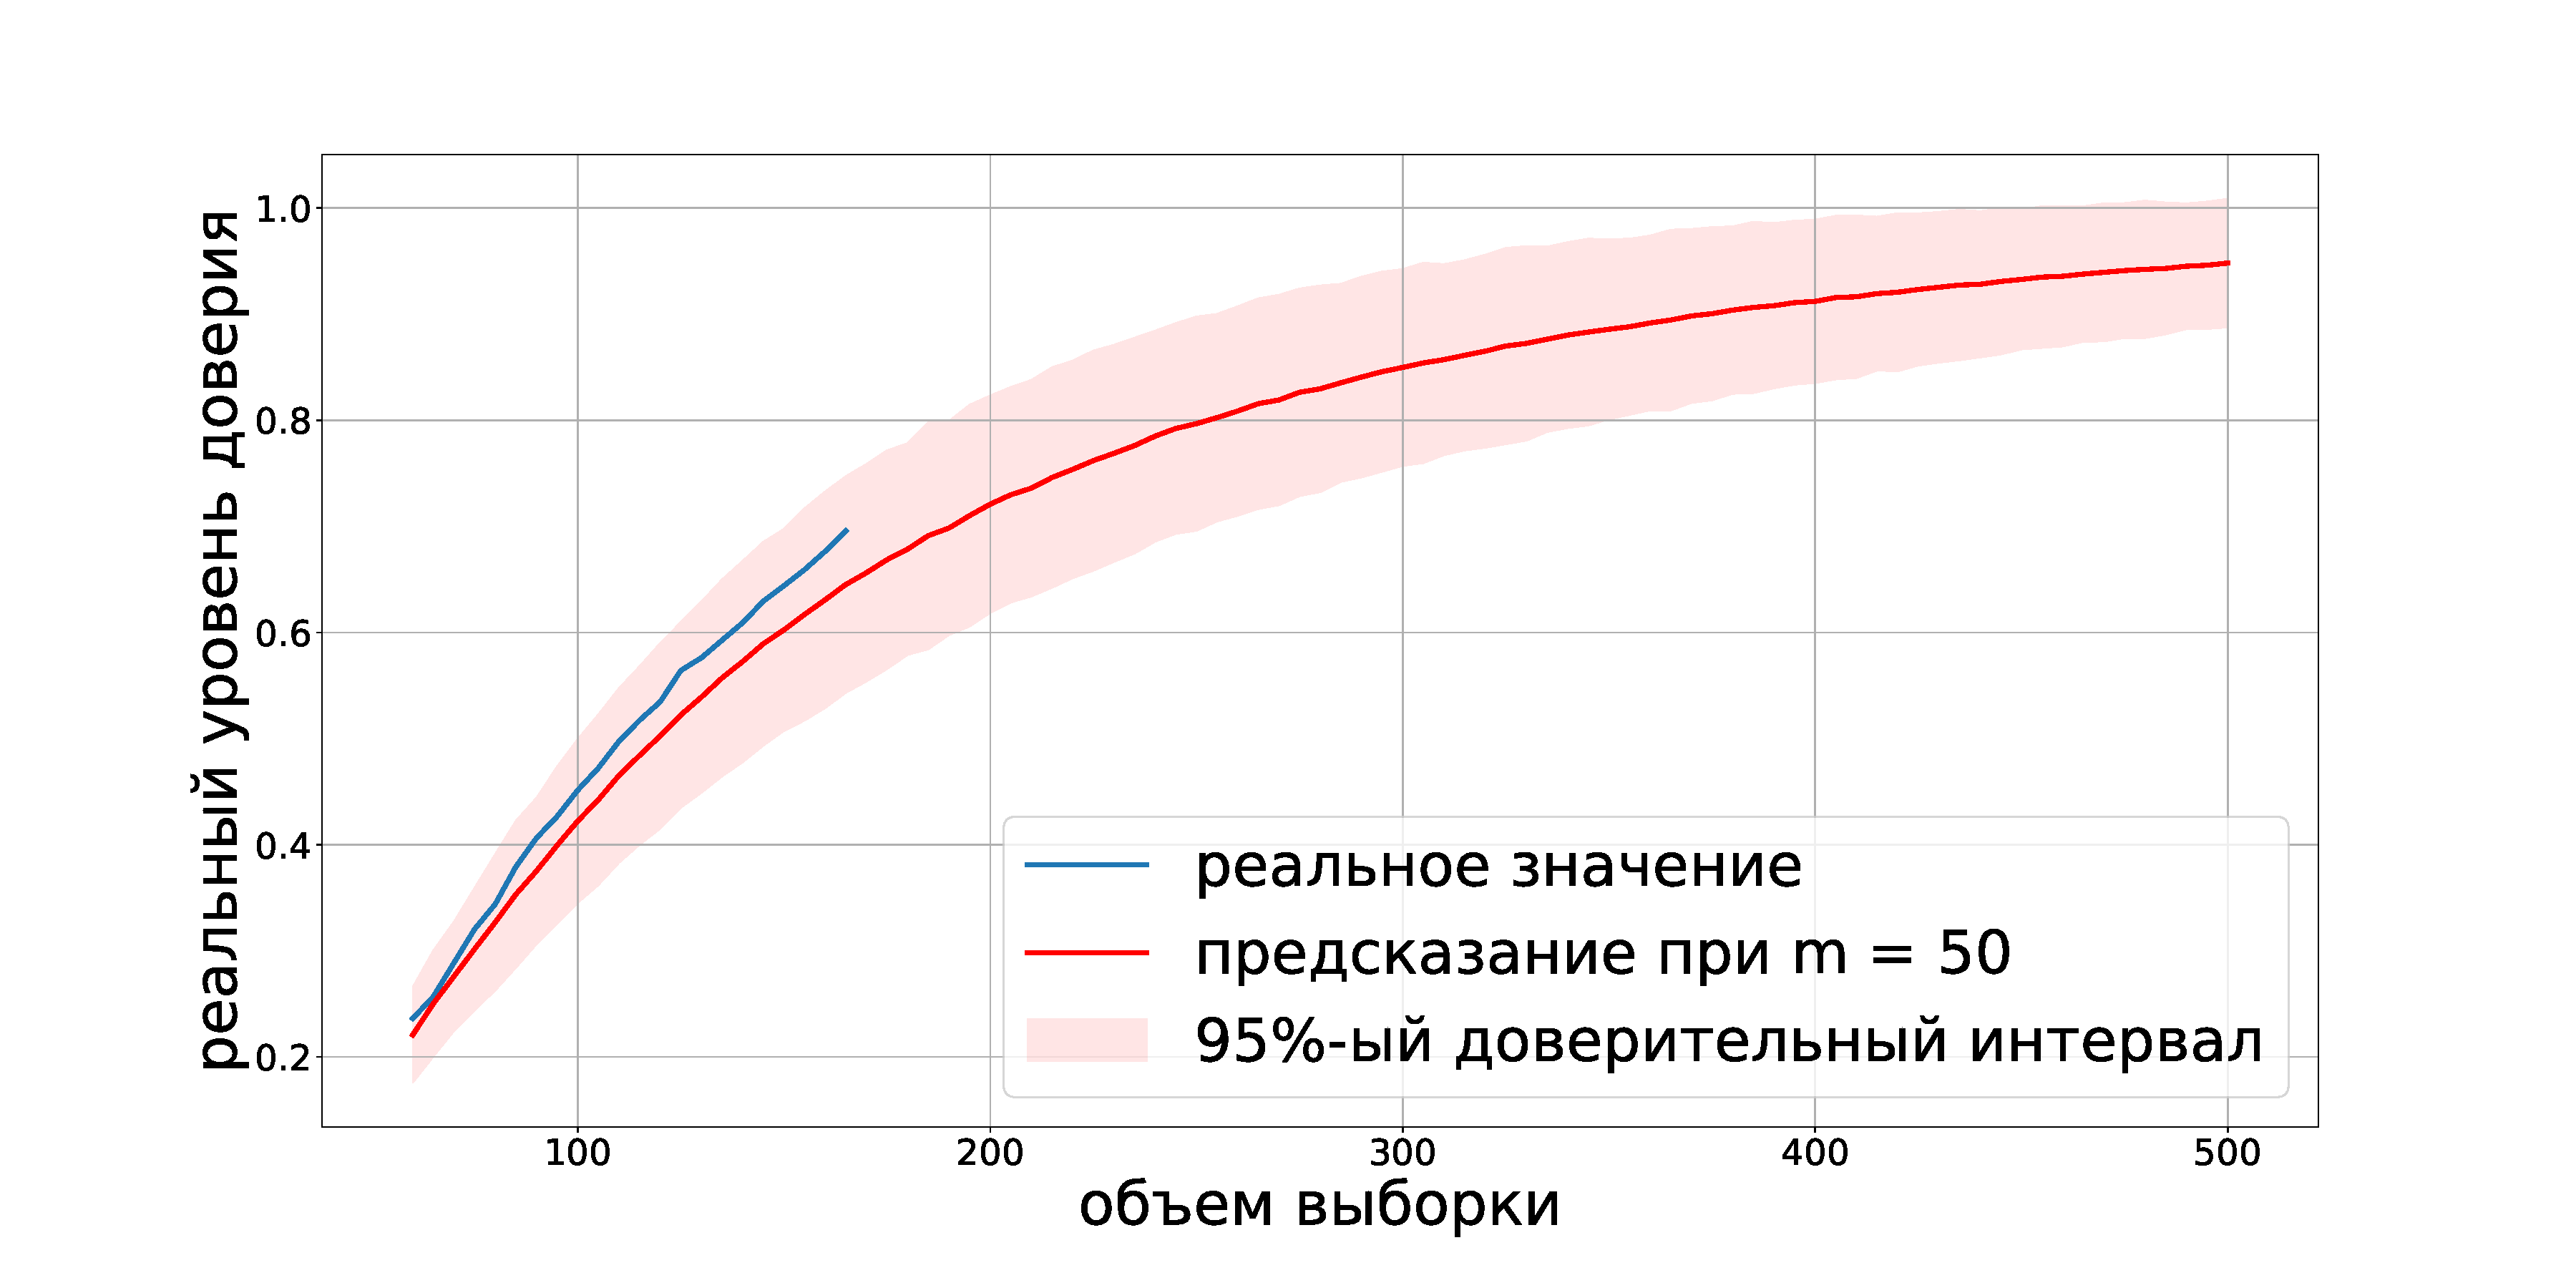
\includegraphics[width=0.5\textwidth]{../data/pics/ACC_modified_servo.pdf}}\\
\subfloat[Boston]{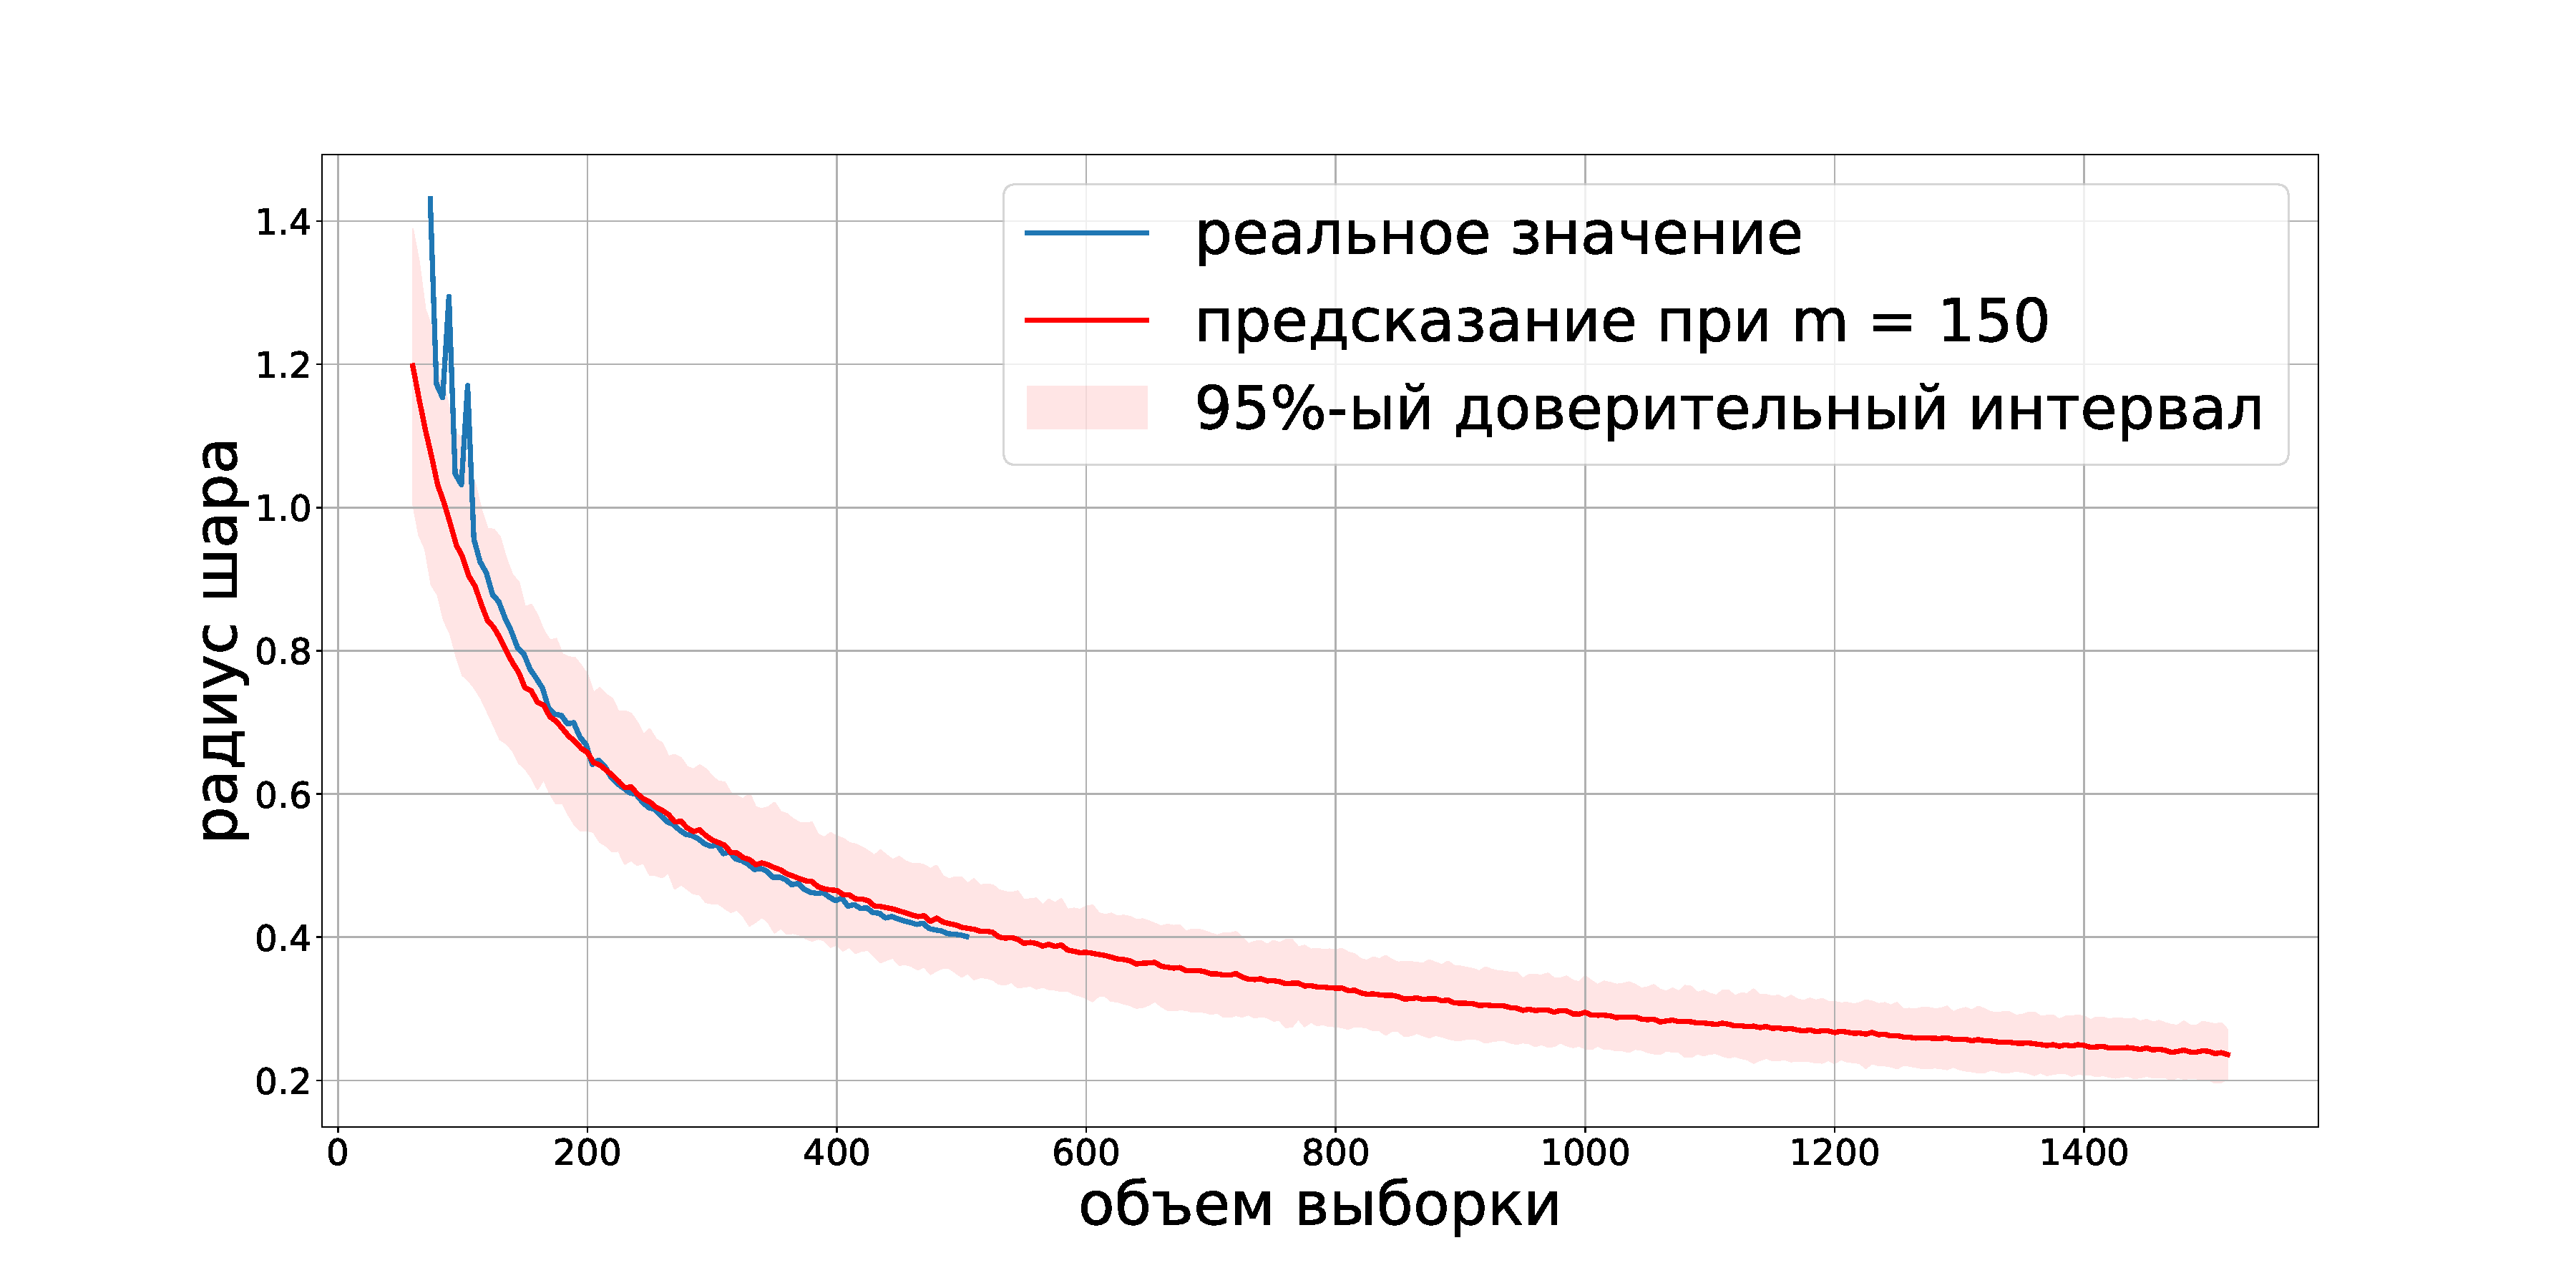
\includegraphics[width=0.5\textwidth]{../data/pics/ALC_modified_boston.pdf}}&
\subfloat[Boston]{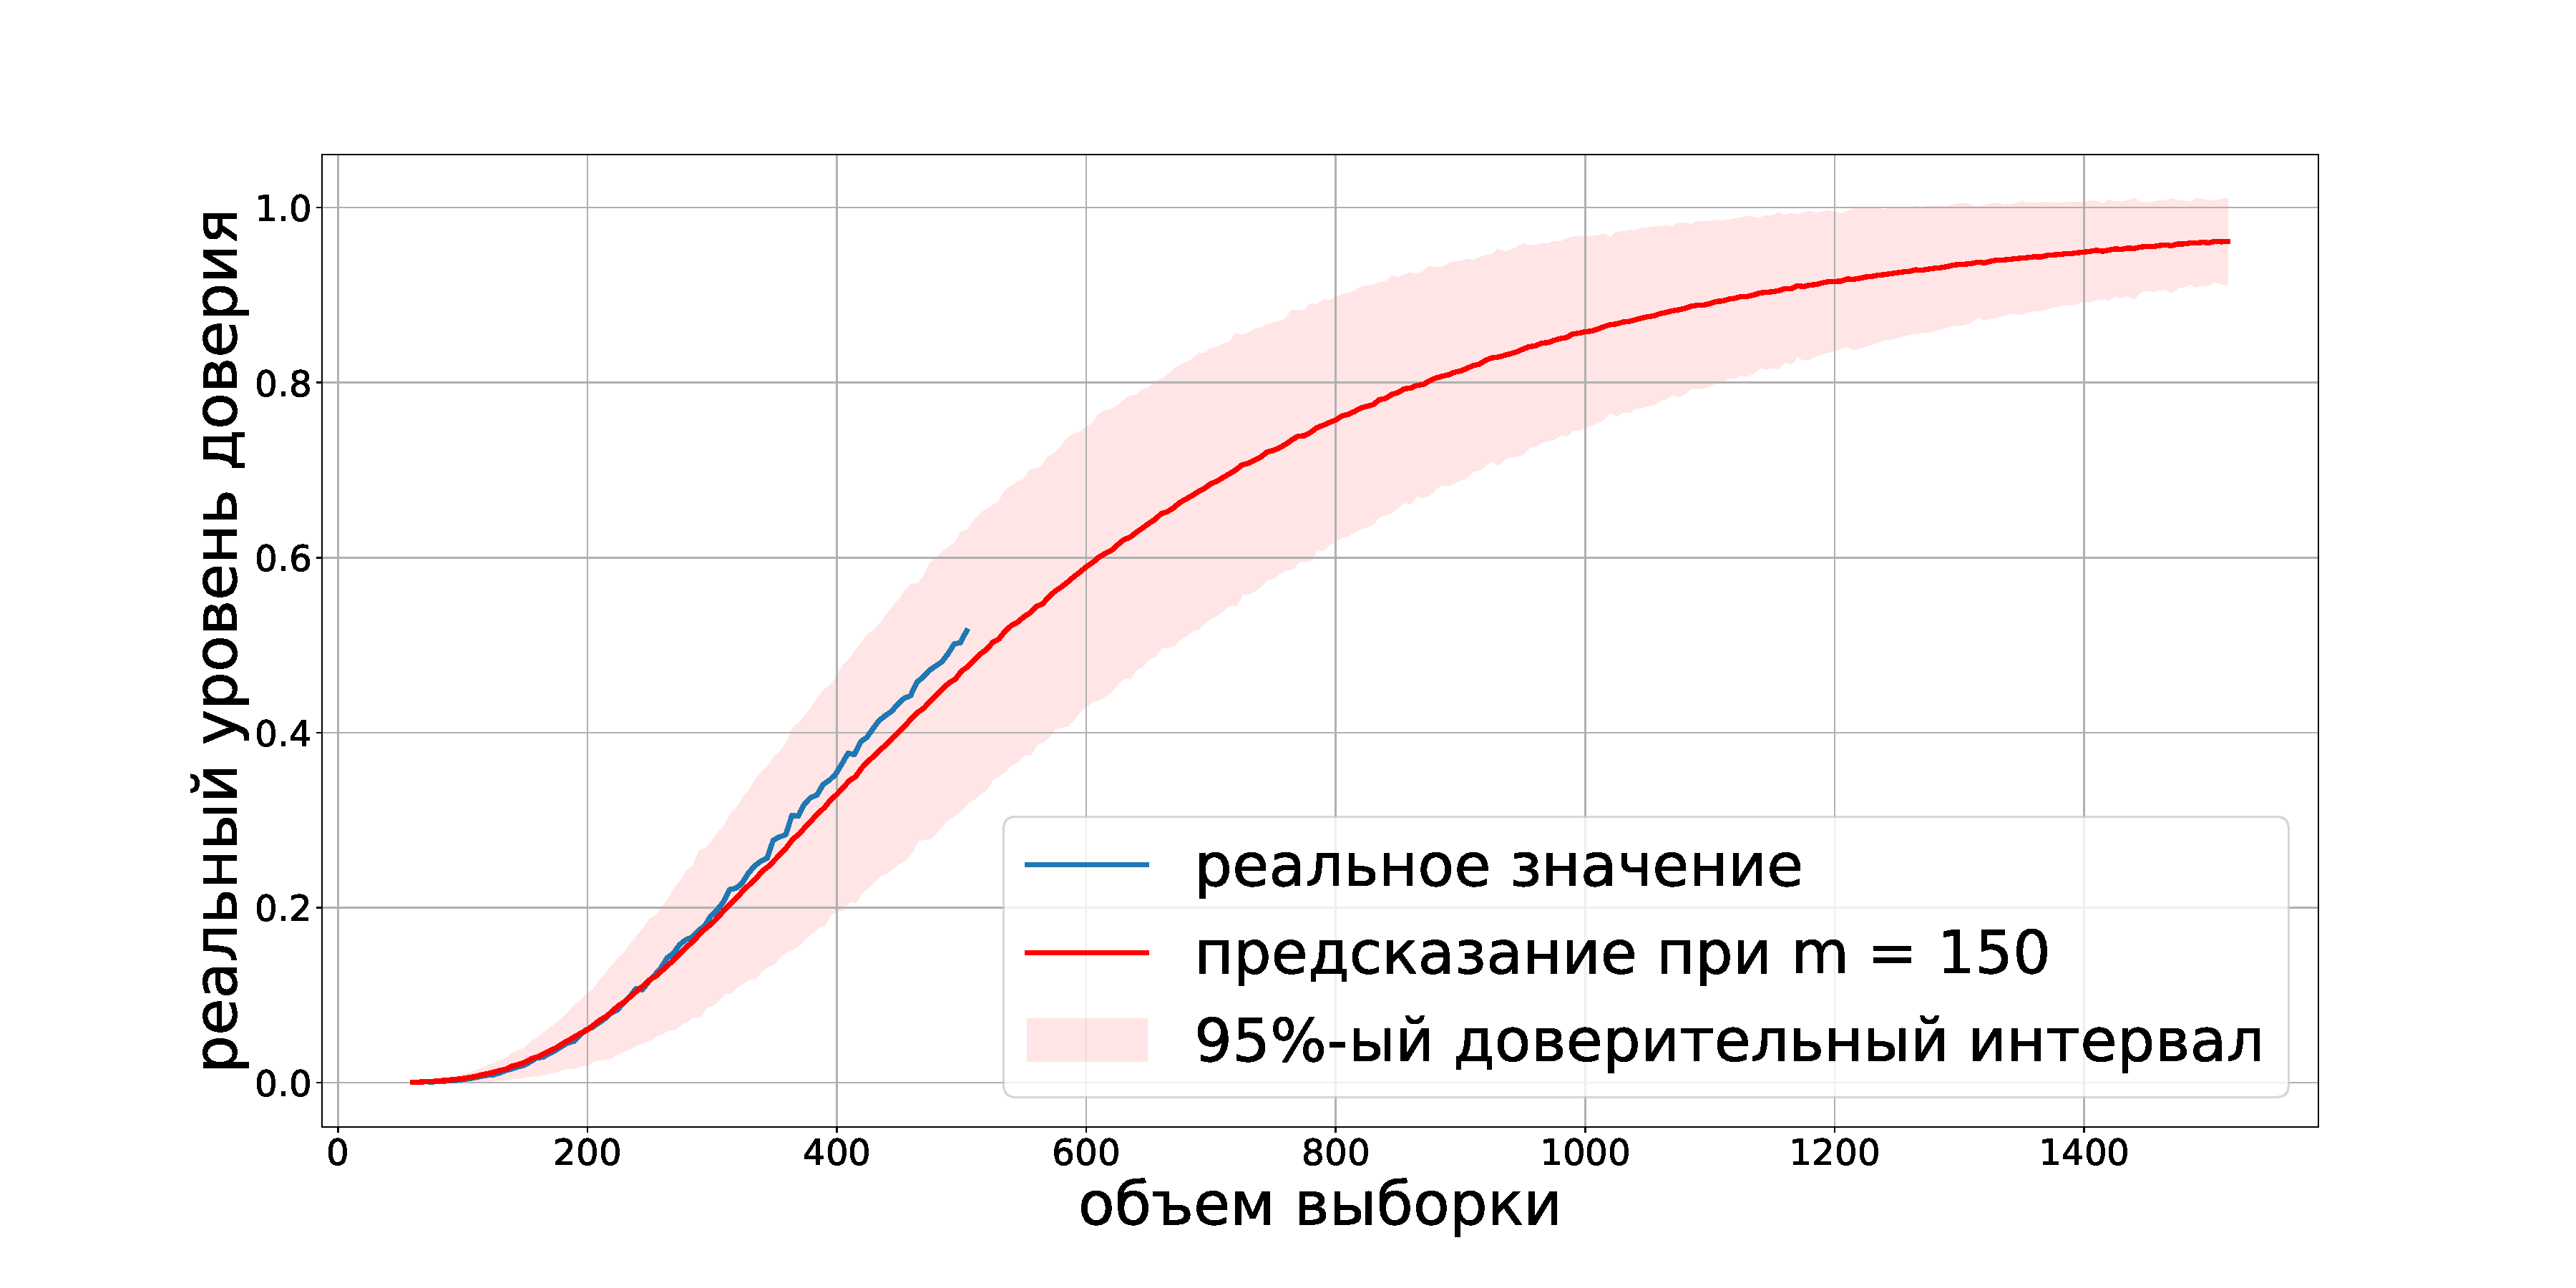
\includegraphics[width=0.5\textwidth]{../data/pics/ACC_modified_boston.pdf}}\\
\subfloat[Diabetes]{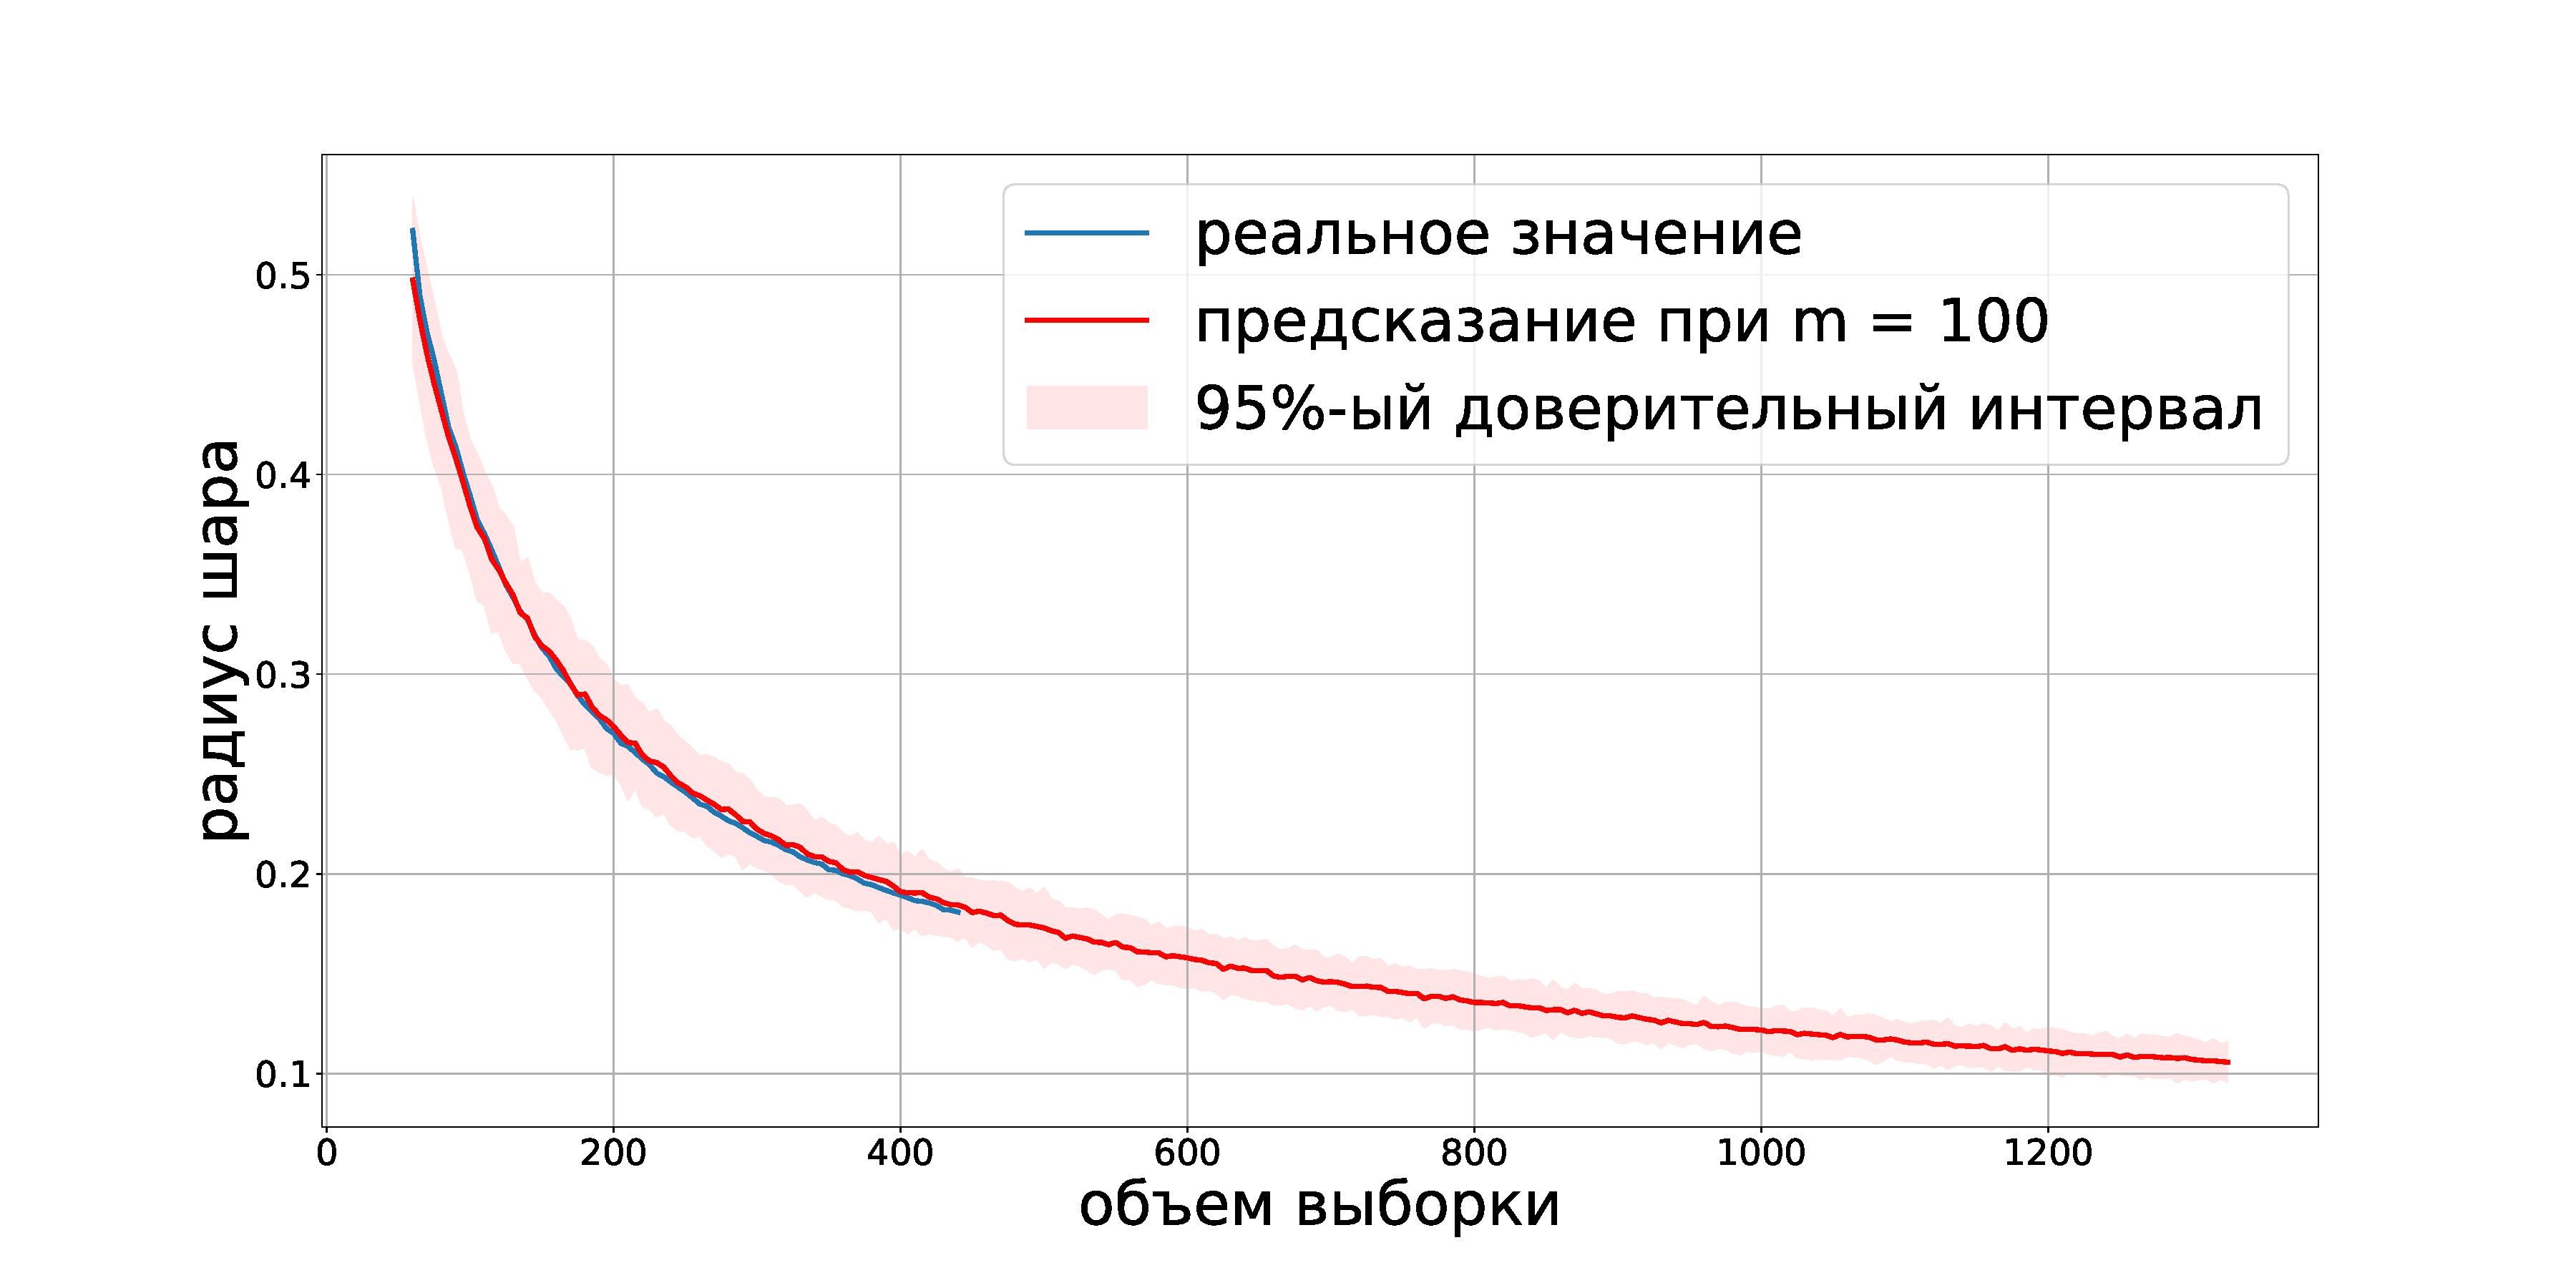
\includegraphics[width=0.5\textwidth]{../data/pics/ALC_modified_diabetes.pdf}}&
\subfloat[Diabetes]{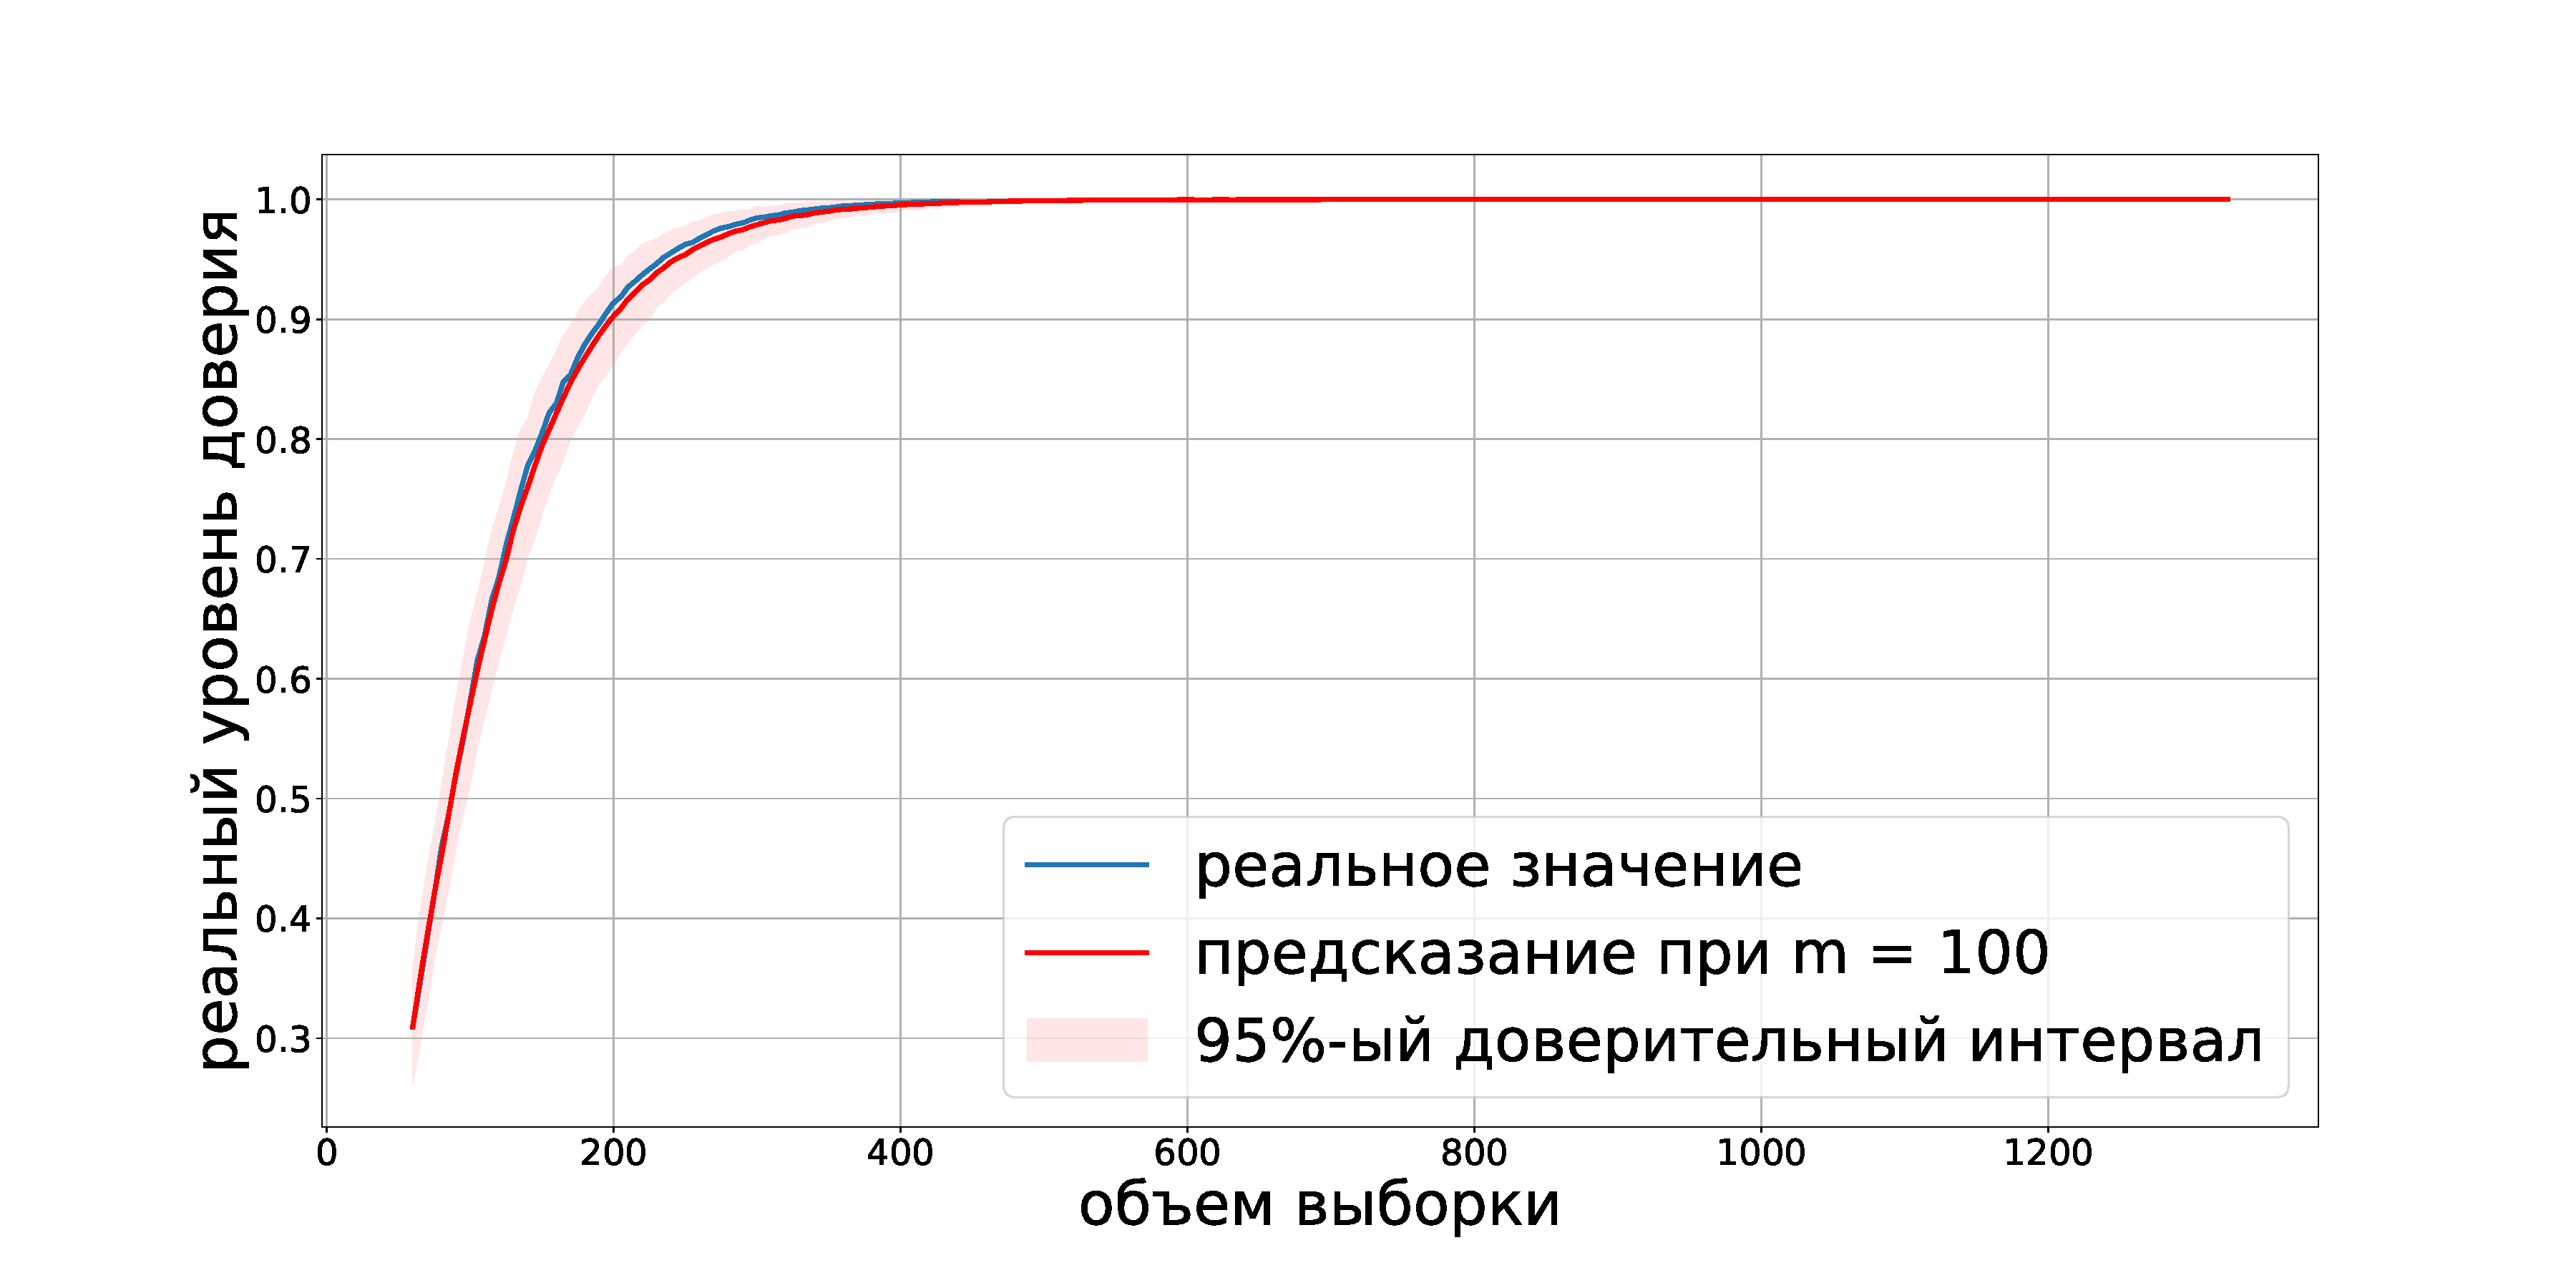
\includegraphics[width=0.5\textwidth]{../data/pics/ACC_modified_diabetes.pdf}}\\
\end{tabular}

\caption{Зависимость значения функции эффективности от объема выборки}
\label{fig100}
\end{figure}

$\newline$
$\newline$
$\newline$
$\newline$
$\newline$
$\newline$
$\newline$

В таблицах 2, 3 представлены результаты предсказания различными методами.


$\newline$

\begin{table}[h]
\begin{center}
\caption{Предсказание достаточного объема выборки, ALC метод}
\label{table2}
\begin{tabularx}{0.7\textwidth}{|p{1in}|X|c|}
\hline
	\centering Выборка & \centering Реальное значение &Предсказание\\
	\hline
	 Servo & \centering не хватает данных & 450\\
	\hline
	Boston & \centering не хватает данных &1370\\
	\hline
	Diabetes & \centering 235 & 240\\
\hline
\end{tabularx}
\end{center}
\end{table}

\begin{table}[h]
\begin{center}
\caption{Предсказание достаточного объема выборки, ACC метод}
\label{table3}
\begin{tabularx}{0.7\textwidth}{|p{1in}|X|c|}
\hline
	\centering Выборка & \centering Реальное значение &Предсказание\\
	\hline
	 Servo & \centering не хватает данных & 405\\
	\hline
	Boston & \centering не хватает данных &1410\\
	\hline
	Diabetes & \centering 235 &245\\
\hline
\end{tabularx}
\end{center}
\end{table}

\bibliographystyle{unsrt}
\bibliography{jmlda-bib}
\begin{thebibliography}{1}


\bibitem{Self-Mauritsen-1998}
\BibAuthor{S.\,G.\;Self and R.\,H.\;Mauritsen}
\BibTitle{Power/sample size calculations for generalized linear
models }~//
\BibJournal{Biometrics}, 1988.

\bibitem{Shieh-2000}
\BibAuthor{G.\,Shieh}
\BibTitle{On power and sample size calculations for likelihood ratio tests in generalized
linear models}~//
\BibJournal{Biometrics}, 2000.

\bibitem{Shieh-2005}
\BibAuthor{G.\,Shieh}
\BibTitle{On power and sample size calculations for Wald tests in generalized linear
models}~//
\BibJournal{Journal of Statistical Planning and Inference}, 2005.


\bibitem{Rubin-Stern-1998}
\BibAuthor{D.\,B.\;Rubin and H.\,S.\;Stern}
\BibTitle{Sample size determination using posterior predictive
distributions }~//
\BibJournal{Sankhya : The Indian Journal of Statistics Special Issue on Bayesian
Analysis}, 1998.

\bibitem{Qumsiyeh-1998}
\BibAuthor{Maher Qumsiyeh}
\BibTitle{Using the bootstrap for estimation the sample size in statistical
experiments }~//
\BibJournal{Journal of modern applied statistical methods}, 2002.

\end{thebibliography}

\end{document}

%ACC diabetes = 245 ???
%ACC boston = 1390
%ACC servo = 455

%ALC diabetes = ???
%ALC boston = ???
%ALC servo = ???


